% Options for packages loaded elsewhere
\PassOptionsToPackage{unicode}{hyperref}
\PassOptionsToPackage{hyphens}{url}
%
\documentclass[
]{article}
\usepackage{amsmath,amssymb}
\usepackage{iftex}
\ifPDFTeX
  \usepackage[T1]{fontenc}
  \usepackage[utf8]{inputenc}
  \usepackage{textcomp} % provide euro and other symbols
\else % if luatex or xetex
  \usepackage{unicode-math} % this also loads fontspec
  \defaultfontfeatures{Scale=MatchLowercase}
  \defaultfontfeatures[\rmfamily]{Ligatures=TeX,Scale=1}
\fi
\usepackage{lmodern}
\ifPDFTeX\else
  % xetex/luatex font selection
\fi
% Use upquote if available, for straight quotes in verbatim environments
\IfFileExists{upquote.sty}{\usepackage{upquote}}{}
\IfFileExists{microtype.sty}{% use microtype if available
  \usepackage[]{microtype}
  \UseMicrotypeSet[protrusion]{basicmath} % disable protrusion for tt fonts
}{}
\makeatletter
\@ifundefined{KOMAClassName}{% if non-KOMA class
  \IfFileExists{parskip.sty}{%
    \usepackage{parskip}
  }{% else
    \setlength{\parindent}{0pt}
    \setlength{\parskip}{6pt plus 2pt minus 1pt}}
}{% if KOMA class
  \KOMAoptions{parskip=half}}
\makeatother
\usepackage{xcolor}
\usepackage[margin=1in]{geometry}
\usepackage{longtable,booktabs,array}
\usepackage{calc} % for calculating minipage widths
% Correct order of tables after \paragraph or \subparagraph
\usepackage{etoolbox}
\makeatletter
\patchcmd\longtable{\par}{\if@noskipsec\mbox{}\fi\par}{}{}
\makeatother
% Allow footnotes in longtable head/foot
\IfFileExists{footnotehyper.sty}{\usepackage{footnotehyper}}{\usepackage{footnote}}
\makesavenoteenv{longtable}
\usepackage{graphicx}
\makeatletter
\def\maxwidth{\ifdim\Gin@nat@width>\linewidth\linewidth\else\Gin@nat@width\fi}
\def\maxheight{\ifdim\Gin@nat@height>\textheight\textheight\else\Gin@nat@height\fi}
\makeatother
% Scale images if necessary, so that they will not overflow the page
% margins by default, and it is still possible to overwrite the defaults
% using explicit options in \includegraphics[width, height, ...]{}
\setkeys{Gin}{width=\maxwidth,height=\maxheight,keepaspectratio}
% Set default figure placement to htbp
\makeatletter
\def\fps@figure{htbp}
\makeatother
\setlength{\emergencystretch}{3em} % prevent overfull lines
\providecommand{\tightlist}{%
  \setlength{\itemsep}{0pt}\setlength{\parskip}{0pt}}
\setcounter{secnumdepth}{5}
\usepackage{tikz}
\usetikzlibrary{calc, positioning}
\usepackage{amsmath}
\usepackage{tikz}
\usepackage{pgfplots}
\usepackage{caption}
\usepackage{subcaption}
\usepackage{cancel}
\usepackage{mathtools}
\usepackage{annotate-equations}
\ifLuaTeX
  \usepackage{selnolig}  % disable illegal ligatures
\fi
\IfFileExists{bookmark.sty}{\usepackage{bookmark}}{\usepackage{hyperref}}
\IfFileExists{xurl.sty}{\usepackage{xurl}}{} % add URL line breaks if available
\urlstyle{same}
\hypersetup{
  pdftitle={Notas de Aulas - MI401},
  pdfauthor={Caio Gomes Alves},
  hidelinks,
  pdfcreator={LaTeX via pandoc}}

\title{Notas de Aulas - MI401}
\usepackage{etoolbox}
\makeatletter
\providecommand{\subtitle}[1]{% add subtitle to \maketitle
  \apptocmd{\@title}{\par {\large #1 \par}}{}{}
}
\makeatother
\subtitle{Probabilidade}
\author{Caio Gomes Alves}
\date{05/2025}

\usepackage{amsthm}
\newtheorem{theorem}{Theorem}[section]
\newtheorem{lemma}{Lemma}[section]
\newtheorem{corollary}{Corollary}[section]
\newtheorem{proposition}{Proposition}[section]
\newtheorem{conjecture}{Conjecture}[section]
\theoremstyle{definition}
\newtheorem{definition}{Definition}[section]
\theoremstyle{definition}
\newtheorem{example}{Example}[section]
\theoremstyle{definition}
\newtheorem{exercise}{Exercise}[section]
\theoremstyle{definition}
\newtheorem{hypothesis}{Hypothesis}[section]
\theoremstyle{remark}
\newtheorem*{remark}{Remark}
\newtheorem*{solution}{Solution}
\begin{document}
\maketitle

% \thispagestyle{empty}
% \begin{tikzpicture}[remember picture, overlay]
%   % Fundo sem gradiente:
%   \shade[top color=blue!30!black, bottom color=blue!30!black]
%     (current page.north west) rectangle (current page.south east);
%
%   % Faixa central
%   \fill[white, opacity=0.2]
%     ([yshift=-3cm]current page.north west) rectangle
%     ([yshift=3cm]current page.south east);
%
%   % Título
%   \node[align=center, text width=0.8\paperwidth, font=\Huge\bfseries, white]
%     at ([yshift=2cm]current page.center)
%     {Notas de Aulas\\MI401 Probabilidade};
%
%   % Autor
%   \node[align=center, text width=0.8\paperwidth, font=\Large, white]
%     at (current page.center)
%     {Caio Gomes Alves};
%
%   % Instituição
%   \node[align=center, text width=0.8\paperwidth, font=\large, white]
%     at ([yshift=-1cm]current page.center)
%     {Instituto de Matemática, Estatística e Computação Científica};
%   \node[align=center, text width=0.8\paperwidth, font=\large, white]
%     at ([yshift=-2cm]current page.center)
%     {Universidade Estadual de Campinas - UNICAMP};
%
%   % Data
%   \node[align=center, font=\large, white]
%     at ([yshift=-4cm]current page.center)
%     {Maio 2025};
%
%   % Elementos gráficos - Curvas de distribuição
%   \draw[white, thick, opacity=0.3] plot[domain=-3:3, smooth]
%     (\x+2,{0.5*exp(-(\x)^2/2)-5});
%   \draw[white, thick, opacity=0.3] plot[domain=0:4, smooth]
%     (\x-6,{0.3*exp(-\x)-4});
% \end{tikzpicture}
% \clearpage

\thispagestyle{empty}
\begin{tikzpicture}[remember picture, overlay]
  % Fundo gradiente
  \shade[top color=blue!30!black, bottom color=blue!30!black]
    (current page.north west) rectangle (current page.south east);

  % Equações matemáticas de fundo
  \node[white, opacity=0.1, anchor=center, scale=3] at (current page.center) {
    $\begin{aligned}
      P\left(\bigcup_{i=1}^{n} A_{i}\right) \le &\sum_{i=1}^{n}P(A_{n}) - \sum_{1 \le i_{1} < i_{2} \le n}P(A_{i_{1}} \cap A_{i_{2}}) + \dots \\
                                                &+ (-1)^{k-1} \sum_{1 \le i_{1} < \dots < i_{k-1} < i_{k}}P(A_{i_{1}} \cap \dots \cap A_{i_{k}}) \\
      &F_{X}(x|A) = \sum_{n}P(A_{n})F_{X}(x|A_{n}) \\
      \Delta_{K,I}(&g(x_{1},\ldots,x_{k})) = g(x_{1},\ldots,x_{k-1},b) - g(x_{1},\ldots,) \\
                                                &J(\underbar{x},\underbar{y}) = \det \begin{bmatrix}
                                                  \frac{\partial x_{1}}{\partial y_{1}} & \cdots & \frac{\partial x_{1}}{\partial y_{n}} \\
                                                  \vdots & \ddots & \vdots \\
                                                  \frac{\partial x_{n}}{\partial y_{1}} & \cdots & \frac{\partial x_{n}}{\partial y_{n}}
                                                \end{bmatrix} \\
      E(X) &= \int_{0}^{\infty}(1 - F(x))dx - \int_{-\infty}^{0}F(x)dx \\
      P(&|X - E(X)| \ge \lambda) \le \frac{\mathrm{Var}(X)}{\lambda^{2}}, \forall \lambda > 0
    \end{aligned}$
  };

  % Conteúdo principal da capa (mesmo código anterior)
  \fill[black, opacity=0.2]
    ([yshift=-3cm]current page.north west) rectangle
    ([yshift=3cm]current page.south east);

  \node[align=center, text width=0.8\paperwidth, font=\Huge\bfseries, white]
    at ([yshift=2cm]current page.center)
    {Notas de Aulas\\MI401 Probabilidade};

    % ... (restante do seu código existente)
    % Autor
  \node[align=center, text width=0.8\paperwidth, font=\Large, white]
    at (current page.center)
    {Caio Gomes Alves};

  % Instituição
  \node[align=center, text width=0.8\paperwidth, font=\large, white]
    at ([yshift=-1cm]current page.center)
    {Instituto de Matemática, Estatística e Computação Científica};
  \node[align=center, text width=0.8\paperwidth, font=\large, white]
    at ([yshift=-2cm]current page.center)
    {Universidade Estadual de Campinas - UNICAMP};

  % Data
  \node[align=center, font=\large, white]
    at ([yshift=-4cm]current page.center)
    {Maio 2025};

\end{tikzpicture}
\cleardoublepage

\renewcommand*\contentsname{Conteúdos}
{
\setcounter{tocdepth}{2}
\tableofcontents
}
\newpage

\hypertarget{prefuxe1cio}{%
\section{Prefácio}\label{prefuxe1cio}}

Este ``livro'' consiste de notas de aulas da matéria MI401 - Probabilidade, do Programa de Mestrado em Estatística, do Instituto de Matemática, Estatística e Computação Científica (IMECC), da Universidade Estadual de Campinas - UNICAMP.

Os seus conteúdos são baseados nas notas tomadas durante as aulas, do livro ``Probabilidade e Variáveis Aleatórias'', do autor Marcos Nascimento Magalhães, 3ª edição, e do livro ``Probabilidade: um curso em nível intermediário'', do autor Barry R. James, 5ª edição.

\newpage

\hypertarget{definiuxe7uxf5es-buxe1sicas}{%
\section{Definições Básicas}\label{definiuxe7uxf5es-buxe1sicas}}

\hypertarget{modelo-probabiluxedstico}{%
\subsection{Modelo Probabilístico}\label{modelo-probabiluxedstico}}

Suponha que é realizado um experimento ``sob certas condições'', sendo \textbf{\(\Omega\)} o conjunto de resultados possíveis do experimento (também chamado de resultados elementares). Chamamos \textbf{\(\Omega\)} de \textbf{espaço amostral do experimento}, com a representação axiomática sendo dada por: \(\Omega = \{\omega : \omega \in \Omega\}\).

\begin{example}
Considere o lançamento de um dado honesto. Nesse caso, temos que \(\Omega = \{1,2,3,4,5,6\}\), em que cada \(\{i\}\) é um evento elementar, sendo eles \{1\},\{2\},\{3\},\{4\},\{5\} e \{6\}.
\end{example}

Temos então que eventos são coleções de pontos em \(\Omega\), por exemplo um evento \(A = \{2,4,6\}\) (números pares no lançamento de um dado honesto). Assim, temos as seguintes suposições para eventos:

\begin{enumerate}
\def\labelenumi{\arabic{enumi}.}
\tightlist
\item
  Todo resultado possível no experimento corresponde a um e somente um \(\omega \in \Omega\);
\item
  Resultados diferentes correspondem a elementos diferentes em \(\Omega\).
\end{enumerate}

\begin{definition}
Seja um espaço amostral \(\Omega\) de um experimento. Todo subconjunto \(A \subset \Omega\) é um evento. \(\Omega\) é o evento certo e \(\emptyset\) é o evento impossível. Além disso, \(\omega \in \Omega \to \{\omega\}\) é um evento elementar.
\end{definition}

Note-se que, dados \(A\) e \(B\) eventos, tais que \(A \subset \Omega\) e \(B \subset \Omega\), temos que:

\begin{itemize}
\tightlist
\item
  \(A \cup B \to (\omega \in A \text{ e } \omega \notin B)\) ou \((\omega \notin A \text{ e } \omega \in B)\) ou \((\omega \in A \text{ e } \omega \in B)\);
\item
  \(A \cap B \to (\omega \in A \cup \omega \in B)\);
\item
  \(A^{c} \to (\omega \notin A)\);
\item
  \(A \subset B \to\) a ocorrência de \(A\) implica a ocorrência de \(B\);
\item
  \(A \cap B = \emptyset \to\) os eventos \(A\) e \(B\) são mutuamente exclusivos.
\end{itemize}

No campo probabilístico, pensamos em atribuir probabilidades (leia-se chances) a eventos em \(\Omega\).

\begin{definition}[Clássica]
A probabilidade de ocorrência de um evento \(A\), denotada por \(P(A)\) é dada por:

\[P(A) = \frac{\#(A)}{\#(\Omega)} = \frac{\text{nº de resultados favoráveis a }A}{\text{nº de resultados possíveis em }\Omega}\]

Onde \(\#\) indica a cardinalidade de um conjunto (quantidade de elementos no conjunto).
\end{definition}

\begin{example}
Seja \(A = \{2,4,6\}\), os lançamentos pares em um dado honesto. Como \(\Omega = \{1,\dots,6\}\), temos que:

\[P(A) = \frac{3}{6} = \frac{1}{2}\]

Note que o conjunto \(A\) pode ser descrito como a união dos eventos elementares, tais que \(A = \{2\} \cup \{4\} \cup \{6\}\). Nesse caso, podemos ver que a probabilidade de \(A\) não muda, pois:

\begin{align*}
P(\{i\}) &= \frac{\#(\{i\})}{\#(\Omega)} = \frac{1}{6}\\
P(A) &= \frac{\#(\{2\})+\#(\{4\})+\#(\{6\})}{\#(\Omega)} = \frac{1+1+1}{6} = \frac{1}{2}
\end{align*}
\end{example}

\begin{definition}
Um evento \(A\) ao qual atribuímos uma probabilidade é um evento aleatório.
\end{definition}

\hypertarget{uxe1lgebras-de-conjuntos}{%
\subsection{Álgebras de Conjuntos}\label{uxe1lgebras-de-conjuntos}}

Considere o conjunto de eventos em uma família \(\mathcal{A}\) (subconjuntos de \(\Omega\)), de tal modo que \(P:A \to [0,1]\). Uma representação gráfica da relação \(P\) pode ser dada por:

\begin{center}
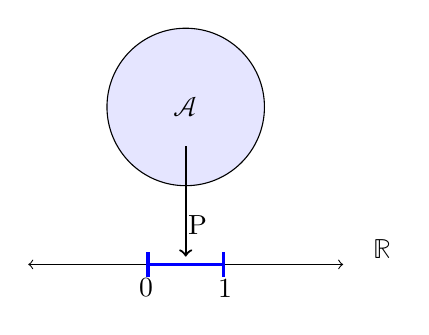
\begin{tikzpicture}
% Desenhando o conjunto A como um círculo:
\draw[fill=blue!10] (0.5,2) circle (1);

% Adicionando o nome do conjunto A:
\node at (0.5,2) {$\mathcal{A}$};

% Desenhando a reta real (-1.5 a 2.5, para ficar simétrico):
\draw[thin, <->] (-1.5,0) -- (2.5,0);
\node at (3, 0.2) {$\mathbb{R}$};

% Desenhando a reta [0,1] de forma a ficar mais aparente:
\draw[|-|, very thick, blue] (0,0) -- (1,0);
\node at (0,-0.3) {$0$};
\node at (1,-0.3) {$1$};

% Desenhando a flecha de A para a reta [0,1]:
\draw[->, thick] (0.5,1.5) -- (0.5,0.1);
\node at (0.65,0.5) {P};
\end{tikzpicture}
\end{center}

\begin{definition}

Seja \(\Omega\) um conjunto não-vazio. Seja \(\mathcal{A}\) uma classe de subconjuntos de \(\Omega\), ela será chamada de \textbf{``Álgebra de subconjuntos de \(\Omega\)''}, caso respeite os seguintes axiomas:

\begin{itemize}
\tightlist
\item
  \(Ax_{1}\) : \(\Omega \in \mathcal{A}\), e definimos \(P(\Omega) = 1\);
\item
  \(Ax_{2}\) : Se \(A \in \mathcal{A} \Rightarrow A^{c} \in \mathcal{A}\), e definimos \(P(A^{c}) = 1 - P(A)\);
\item
  \(Ax_{3}\) : Se \(A \in \mathcal{A}, B \in \mathcal{A} \Rightarrow A \cup B \in \mathcal{A}\).
\end{itemize}

E por consequência desses axiomas, temos as seguintes extensões:

\begin{itemize}
\tightlist
\item
  \(Ax_{4}\) : \(\emptyset \in \mathcal{A}\);
\item
  \(Ax_{5}\) : Sejam \(A_{1}, A_{2}, \dots, A_{n} : A_{i} \in \mathcal{A} \forall i \Rightarrow \bigcup_{i=1}^{n}A_{i} \in \mathcal{A}\) e \(\bigcap_{i = 1}^{n}A_{i} \in \mathcal{A}\).
\end{itemize}

\end{definition}

É fácil verificar a extensão de \(Ax_{4}\) a partir de \(Ax_{1} \text{ e } Ax_{2}\): \(Ax_{1}\) define que \(\Omega \in \mathcal{A}\), e por \(Ax_{2}\) temos que \(\Omega^{c} \in \mathcal{A}\), e por definição temos que \(\Omega^{c} = \emptyset\), logo \(\emptyset \in \mathcal{A}\). Também é interessante notar que, ainda por \(Ax_{2}\), temos que \(P(\emptyset) = 1 - P(\Omega)\), e por \(Ax_{1}\) temos que \(P(\Omega) = 1\), portanto \(P(\emptyset) = 1 - 1 = 0\).

A extensão de \(Ax_{5}\) é dada por indução e pelas Leis de De Morgan: Sejam \(A_{1}, A_{2} \in \mathcal{A}\). Temos pelo axioma \(Ax_{3}\), que \(A_{1} \cup A_{2} \in \mathcal{A}\), podendo assim definir o conjunto \(B = A_{1} \cup A_{2}\), sendo possível ver que \(B \in \mathcal{A}\). Sejam ainda um conjunto \(A_{3} \in \mathcal{A}\), podemos ver que \(B \cup A_{3} \in \mathcal{A}\), e como \(B = A_{1} \cup A_{2}\), temos que \((A_{1} \cup A_{2}) \cup A_{3} \in \mathcal{A}\). Podemos proceder dessa forma para qualquer quantidade (enumerável) de conjuntos, de modo que \(\bigcup_{i = 1}^{n}A_{i} \in \mathcal{A}\). Pelas Leis de De Morgan, sabemos que:

\begin{equation}
\bigcap_{i=1}^{n}A_{i} = \left(\bigcup_{i = 1}^{n}A_{i}^{c}\right)^{c}
\label{eq:demorgan}
\end{equation}

E pela extenção indutiva em \(n\) do axioma \(Ax_{2}\), temos que se \(A_{i}^{c} \in \mathcal{A}, \forall i\), então \(\bigcup_{i = 1}^{n}A_{i}^{c} \in \mathcal{A}\). E como, se um conjunto pertence a \(\mathcal{A}\) seu complementar deve pertencer também, e pelo resultado em \eqref{eq:demorgan}, temos então que:

\begin{equation}
\left(\bigcup_{i = 1}^{n}A_{i}^{c}\right)^{c} = \left(\bigcap_{i = 1}^{n}A_{i}\right) \in \mathcal{A}
\label{eq:axioma5}
\end{equation}

Assim provamos o axioma \(A_{5}\) como extensão indutiva dos axiomas anteriores, indicando que tanto a união quanto a interseção dos \(A_{i}\) pertencem à \(\mathcal{A}\). Podemos também mostrar que a álgebra \(\mathcal{A}\) é fechada também para a operação de diferença entre conjuntos: \(A \in \mathcal{A}, B \in \mathcal{A}, A-B = A \cap B^{c} \in \mathcal{A}\).

\begin{proof}[Prova]
Considerando que os conjuntos \(A\) e \$B pertencem à \(\mathcal{A}\), podemos utilizar o axioma \(Ax_{2}\) para mostrar que \(A^{c} \in \mathcal{A}\) e \(B^{c} \in \mathcal{A}\). A partir disso, por meio do axioma \(Ax_{5}\) temos que os seguintes conjuntos também pertencem à \(\mathcal{A}\): \(A \cup B, A \cup B^{c}, A^{c} \cup B, A^{c} \cup B^{c}, A \cap B, A \cap B^{c}, A^{c} \cap B, A^{c} \cap B^{c}\). E como temos que \(A \cap B^{c} = A-B\), temos a prova de que \(A-B \in \mathcal{A}\). Além disso, essa prova mostra que a diferença contrária (\(B - A = A^{c} \cap B\)) também pertence à algebra \(\mathcal{A}\).
\end{proof}

Ainda considerando os conjuntos \(A\) e \(B\), existem cinco maneiras como esses conjuntos podem ``interagir'', e podemos mostrar que em todos os casos a diferença \(A-B \in \mathcal{A}\):

\begin{itemize}
\tightlist
\item
  \(A \not\subset B\) e \(A \not\supset B\) e \(A \cap B \neq \emptyset \Rightarrow A-B = A \cap B^{c} \in \mathcal{A}\);
\item
  \(A \not\subset B\) e \(A \not\supset B\) e \(A \cap B = \emptyset \Rightarrow A-B = A \in \mathcal{A}\);
\item
  \(A \supset B \Rightarrow A-B = A \cap B^{c} \in \mathcal{A}\);
\item
  \(A \subset B \Rightarrow A-B = \emptyset \in \mathcal{A}\);
\item
  \(A = B \Rightarrow A-B = \emptyset \in \mathcal{A}\).
\end{itemize}

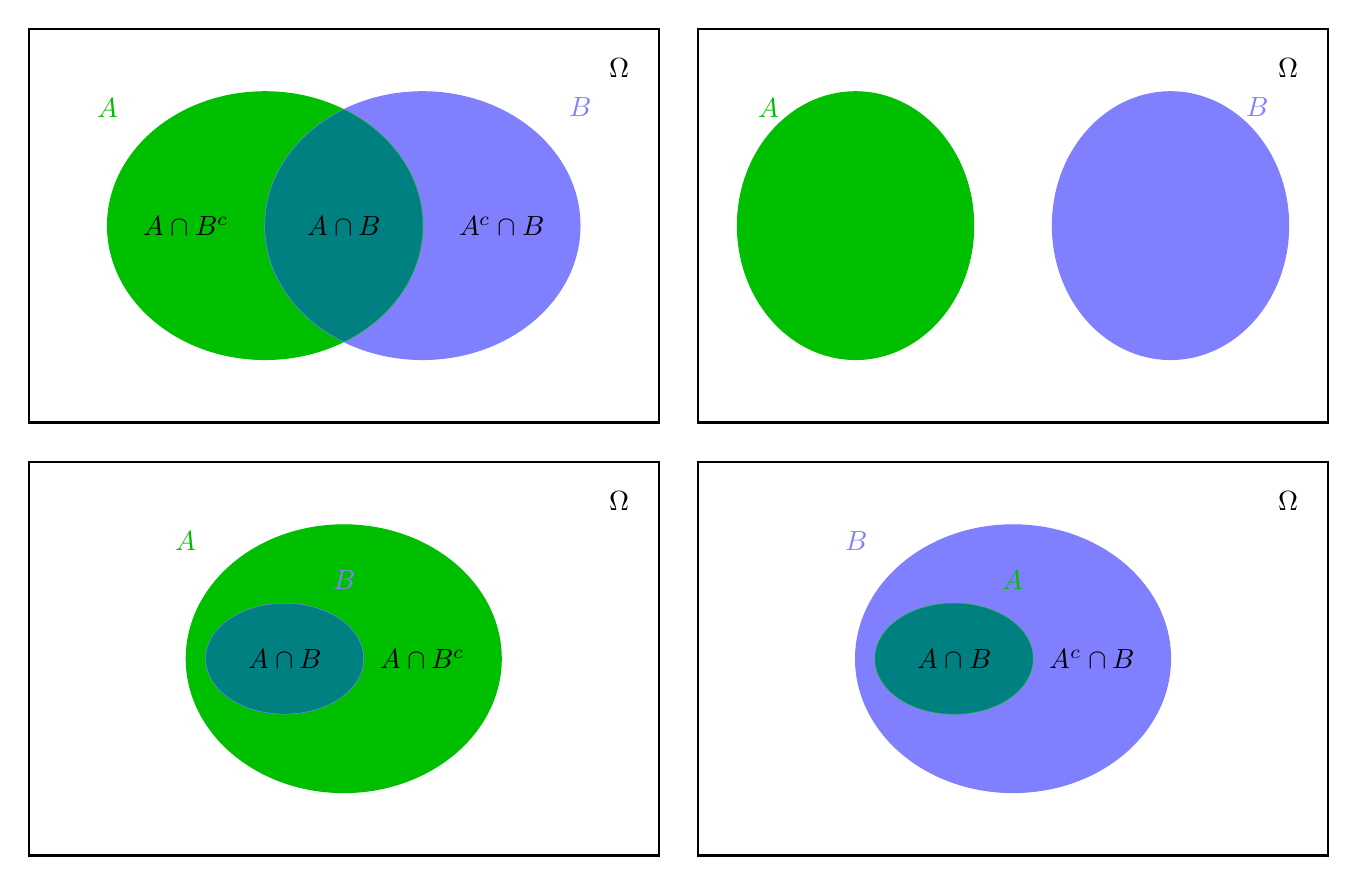
\begin{tikzpicture}
\centering
    % Primeira figura:
    \begin{scope}
    \draw[thick] (0,0) rectangle (8,5);
    \node (n0) at (7.5,4.5) {$\Omega$};
    \def\first{(3,2.5) ellipse (2 cm and 1.7 cm)};
    \def\second{(5,2.5) ellipse (2 cm and 1.7 cm)};
    \fill[fill=green!75!black]\first;
    \fill[fill=blue!50!white]\second;
    \draw[color=green!75!black] \first;
    \draw[color=blue!50!white] \second;
    \begin{scope}
        \clip \first;
        \fill[fill=green!50!blue]\second;
    \end{scope}
    \node (n1) at (1,4) {\textcolor{green!75!black}{$A$}};
    \node (n2) at (7,4) {\textcolor{blue!50!white}{$B$}};
    \node (n3) at (2,2.5) {$A \cap B^{c}$};
    \node (n4) at (6,2.5) {$A^{c} \cap B$};
    \node (n5) at (4,2.5) {$A \cap B$};
    \end{scope}
    % Início da segunda figura:
        \begin{scope}[xshift=8.5cm]
    \draw[thick] (0,0) rectangle (8,5);
    \node (n0) at (7.5,4.5) {$\Omega$};
    \def\first{(2,2.5) ellipse (1.5 cm and 1.7 cm)};
    \def\second{(6,2.5) ellipse (1.5 cm and 1.7 cm)};
    \fill[fill=green!75!black]\first;
    \fill[fill=blue!50!white]\second;
    \draw[color=green!75!black] \first;
    \draw[color=blue!50!white] \second;
    \begin{scope}
        \clip \first;
        \fill[fill=green!50!blue]\second;
    \end{scope}
    \node (n1) at (0.9,4) {\textcolor{green!75!black}{$A$}};
    \node (n2) at (7.1,4) {\textcolor{blue!50!white}{$B$}};
    \end{scope}
    % Início da terceira figura:
    \begin{scope}[yshift=-5.5cm]
    \draw[thick] (0,0) rectangle (8,5);
    \node (n0) at (7.5,4.5) {$\Omega$};
    \def\first{(4,2.5) ellipse (2 cm and 1.7 cm)};
    \def\second{(3.25,2.5) ellipse (1 cm and 0.7 cm)};
    \fill[fill=green!75!black]\first;
    \fill[fill=blue!50!white]\second;
    \draw[color=green!75!black] \first;
    \draw[color=blue!50!white] \second;
    \begin{scope}
        \clip \first;
        \fill[fill=green!50!blue]\second;
    \end{scope}
    \node (n1) at (2,4) {\textcolor{green!75!black}{$A$}};
    \node (n2) at (4,3.5) {\textcolor{blue!50!white}{$B$}};
    \node (n3) at (3.25,2.5) {$A \cap B$};
    \node (n4) at (5,2.5) {$A \cap B^{c}$};
    \end{scope}
    % Início da quarta figura:
    \begin{scope}[xshift=8.5cm,yshift=-5.5cm]
    \draw[thick] (0,0) rectangle (8,5);
    \node (n0) at (7.5,4.5) {$\Omega$};
    \def\first{(4,2.5) ellipse (2 cm and 1.7 cm)};
    \def\second{(3.25,2.5) ellipse (1 cm and 0.7 cm)};
    \fill[fill=blue!50!white]\first;
    \fill[fill=green!75!black]\second;
    \draw[color=blue!50!white] \first;
    \draw[color=green!75!black] \second;
    \begin{scope}
        \clip \first;
        \fill[fill=green!50!blue]\second;
    \end{scope}
    \node (n1) at (2,4) {\textcolor{blue!50!white}{$B$}};
    \node (n2) at (4,3.5) {\textcolor{green!75!black}{$A$}};
    \node (n3) at (3.25,2.5) {$A \cap B$};
    \node (n4) at (5,2.5) {$A^{c} \cap B$};
    \end{scope}
\label{diagramasvenn}
\end{tikzpicture}
\captionof{figure}{Diferentes relações entre $A$ e $B$ demonstradas por Diagramas de Venn. Note que em todos os casos, $A \cap B^{c} \in \mathcal{A}$ ou $A \cap B^{c} = \emptyset \in \mathcal{A} \text{ ou } A \cap B^{c} = A \in \mathcal{A}$}

As representações por Diagramas de Venn apresentadas na figura \ref{diagramasvenn} não é prova formal de que a álgebra \(\mathcal{A}\) é fechada para a diferença, mas é um recurso visual que pode auxiliar no entendimento da relação entre os conjuntos.

\begin{definition}
Uma classe \(\mathcal{A}\) de conjuntos/subconjuntos de \(\Omega \neq \emptyset\), verificando os axiomas \(Ax_{1}, Ax_{2} \text{ e } Ax_{3}\) é chamada de \(\sigma\)-álgebra de subconjuntos de \(\Omega\).
\end{definition}

Note que uma \(\sigma\)-álgebra é sempre uma álgebra. Uma outra forma de construir \(\sigma\)-álgebras é partir de uma álgebra munida dos axiomas de Kolmogorov (Teorema de Carathéodory).

\begin{proposition}
Seja \(\mathcal{A}\) uma \(\sigma\)-álgebra de subconjuntos de \(\Omega\), se \(A_{1}, A_{2},\dots,\) é uma coleção em \(\mathcal{A} \Rightarrow \bigcap_{i=1}^{\infty}A_{n} \in \mathcal{A}\).
\end{proposition}

\begin{example}
\protect\hypertarget{exm:powerset}{}\label{exm:powerset}Seja \(\Omega = \{1,2,3,4,5,6\}\) (o lançamento de um dado cúbico usual). A \(\sigma\)-álgebra usual é definida da seguinte forma e denotada por \(\mathcal{P}(\Omega)\) (chamada de partes de \(\Omega\) ou \emph{powerset} de \(\Omega\)):

\begin{align*}
\mathcal{A} = \{&\emptyset,\{1\},\{2\},\{3\},\{4\},\{5\},\{6\},\\
& \{1,2\},\{1,3\},\{1,4\},\{1,5\},\{1,6\}, \\
&\{2,3\},\{2,4\},\dots,\\
&\Omega\}
\end{align*}
\end{example}

\begin{example}
Definamos a \(\sigma\)-álgebra de Borel no intervalo \(\Omega = [0,1]\). Uma possível definição seria:

\[
\mathcal{A} = \text{ todos os subconjuntos de } [0,1] \text{ cujo cumprimento esteja bem definido}
\]

Podemos, por exemplo, propor uma álgebra para o intervalo \([0,1]\) dada por:

\[
\mathcal{A_{0}} = \{A \subset [0,1]: A \text{ é uma união finita de intervalos }\}
\]

É possível encontrar um conjunto \(A\) tal que \(A \not\in \mathcal{A}\), por exemplo:

\[
A = \left\{\left(0,\frac{1}{2}\right) \cup \left(\frac{1}{2},\frac{3}{4}\right)\cup \dots \cup \left(1-\frac{1}{2^{n}},1-\frac{1}{2^{n+1}}\right)\cup \dots\right\}
\]

Podemos ver que, para qualquer \(n^{*}\) finito, \(\lim_{n \to n^{*}}\left(1 - \frac{1}{2^{n+1}}\right) \neq 1\), de modo que o conjunto \(A\) não cobrirá completamente o intervalo \([0,1]\). Dessa forma, a \(\sigma\)-álgebra de Borel no intervalo \([0,1]\) (denotada \(\mathcal{B}_{[0,1]}\)) é definida como:

\[
\mathcal{B}_{[0,1]} = \left\{A: A \subset [0,1] \text{ e }A \text{ é boreliano}\right\}
\]

Onde boreliano denota que \(A\) é união enumerável (finita ou infinita) de intervalos em \([0,1]\)
\end{example}

\hypertarget{axiomas-de-kolmogorov}{%
\subsection{Axiomas de Kolmogorov}\label{axiomas-de-kolmogorov}}

Seja \(P:\mathcal{A} \rightarrow [0,1]\), com:

\begin{itemize}
\tightlist
\item
  \(Ax_{1}(K): P(A) \ge 0, \forall A \in \mathcal{A}\);
\item
  \(Ax_{2}(K): P(\Omega) = 1\);
\item
  \(Ax_{3}(K):\) Se \(A_{1},A_{2},\dots,A_{n} : A_{i} \in \mathcal{A} \forall i\) e \(A_{i} \cap A_{j} = \emptyset \forall i,j \in \{1,2,\dots,n\}, i \neq j \Rightarrow P\left(\bigcup_{k=1}^{n}A_{k}\right) = \sum_{k=1}^{n}P(A_{k})\).
\end{itemize}

\begin{definition}

Seja \(\Omega\) um conjunto não-vazio, \(\mathcal{A}\) uma \(\sigma\)-álgebra em \(\Omega\), com \(P : \mathcal{A} \to [0,1]\), verificando os axiomas de Kolmogorov, então \(P\) é dita finitamente aditiva. Podemos assim, modificar o axioma \(Ax_{3}(K)\) para:

\begin{itemize}
\tightlist
\item
  \(Ax'_{3}(K):\) Se \(A_{1},A_{2},\dots\) é uma sequência em \(\mathcal{A}\) tal que \(\forall i \neq j, A_{i} \cap A_{j} = \emptyset\), tem-se que \(P\left(\bigcup_{n=1}^{\infty}A_{n}\right) = \sum_{n=1}^{\infty}P(A_{n})\). (\emph{propriedade da \(\sigma\)-aditividade})
\end{itemize}

\end{definition}

\begin{definition}
\(P\) definida em uma \(\sigma\)-álgebra \(\mathcal{A}\), satisfazendo os axiomas de Kolmogorov (\(Ax_{1}(K), Ax_{2}(K), Ax'_{3}(K)\)) é uma medida de probabilidade em \(\mathcal{A}\), constituída pela terna \((\Omega, \mathcal{A},P)\).
\end{definition}

\hypertarget{propriedades-da-medida-de-probabilidade}{%
\subsection{Propriedades da medida de probabilidade}\label{propriedades-da-medida-de-probabilidade}}

\begin{proposition}[Continuidades]
\protect\hypertarget{prp:continuidade}{}\label{prp:continuidade}\leavevmode

\begin{enumerate}
\def\labelenumi{\arabic{enumi}.}
\tightlist
\item
  Seja \(\{A_{i}\}_{i=1}^{\infty}\) uma sequência (crescente) de eventos tais que \(A_{1} \subseteq A_{2} \subseteq A_{3} \subseteq \dots\), e seja \(A = \bigcup_{i=1}^{\infty}A_{i}\), então \(P(A) = \lim_{i \to \infty}P(A_{i})\).
\item
  Seja \(\{B_{i}\}_{i=1}^{\infty}\) uma sequência (decrescente) de eventos tais que \(B_{1} \supseteq B_{2} \supseteq B_{3} \supseteq \dots\), e seja \(B = \bigcap_{i=1}^{\infty}B_{i}\), então \(P(B) = \lim_{i \to \infty}P(B_{i})\).
\end{enumerate}

\end{proposition}

\begin{proof}[Prova]
\leavevmode

\begin{enumerate}
\def\labelenumi{\arabic{enumi}.}
\tightlist
\item
  Note que, sendo \(A_{0} = \emptyset\), tem-se que \(A = (A_{1} - A_{0}) \cup (A_{2} - A_{1}) \cup (A_{3} - A_{2}) \cup \dots\), ou seja, \(A\) é união disjunta de eventos \(D_{i} = A_{i} - A_{i-1}\), de forma que \(A_{i-1} \subseteq A_{i} \Rightarrow P(A_{i}) = P(A_{i-1}) + P(A_{i} - A_{i-1}) \Rightarrow P(A_{i} - A_{i-1}) = P(A_{i}) - P(A_{i-1})\). Logo, temos que:
\end{enumerate}

\begin{align*}
A = \bigcup_{i=1}^{\infty}D_{i} \xRightarrow{Ax'_{3}(K)} P(A) &= \sum_{i=1}^{\infty}P(D_{i})\\
&= \sum_{i=1}^{\infty}P(A_{i} - A_{i-1})\\
&= \lim_{n \to \infty} \sum_{i=1}^{n} \left[P(A_{i}) - P(A_{i-1})\right] \\
&= \lim_{n \to \infty} \left[P(A_{1}) - P(A_{0}) + P(A_{2}) - P(A_{1}) + P(A_{3}) - P(A_{2}) + \dots\right]\\
&= \lim_{n \to \infty} P(A_{n})
\end{align*}

\begin{enumerate}
\def\labelenumi{\arabic{enumi}.}
\setcounter{enumi}{1}
\tightlist
\item
  Note que, por De Morgan, \(B = \bigcap_{i=1}^{n}B_{i} = \left(\bigcup_{i=1}^{n}B_{i}^{c}\right)^{c}\). Logo \(P(\bigcap_{i=1}^{n}B_{i}) = 1 - P(\bigcup_{i = 1}^{n}B_{i}^{c})\). Seja \(A = B_{i}^{c}\) de modo que:
\end{enumerate}

\begin{align*}
B_{1}^{c} &= \Omega - B_{1} = A_1 \\
B_{2}^{c} &= (B_{1} - B_{2}) \cup (\Omega - B_{1}) = A_{2} \\
&\;\;\vdots
\end{align*}

Assim \(A_{1} \subseteq A_{2} \subseteq A_{3} \subseteq \dots\), e com isso \(P(\bigcap_{i=1}^{n}B_{i}) = 1 - P(\bigcup_{i=1}^{n}B_{i}^{c}) = 1 - P(\bigcup_{i = 1}^{n}A_{i})\). Por outro lado, tem-se que \(A = \bigcup_{i = 1}^{\infty}A_{i} = \bigcup_{i=1}^{\infty}B_{i}^{c} \Rightarrow A^{c} = \left(\bigcup_{i=1}^{\infty}B_{i}^{c}\right)^{c} = \bigcap_{i=1}^{\infty} B_{i} = B\). Logo, temos que:

\[
P\left(\bigcap_{i=1}^{n}B_{i}\right) \xrightarrow[n \to \infty]{} (1 - P(A)) = P(A^{c}) = P(B)
\]

\end{proof}

\begin{definition}[Continuidade no vazio]
\leavevmode

\begin{itemize}
\tightlist
\item
  \(Ax_{4}(K)\) : Se \(\{A_{n}\}_{n \ge 1} \subseteq \mathcal{A}\) e \(A_{n} \supseteq A_{n+1} \forall n\) e \(\bigcap_{n+1}^{\infty}A_{n} \neq \emptyset\) então \(P(A_{n}) \xrightarrow[n \to \infty]{} 0\)
\end{itemize}

\end{definition}

A prova dessa definição é dada pela segunda parte da prova da proposição \ref{prp:continuidade}. A representação visual é dada pelo seguinte diagrama:

\begin{center}
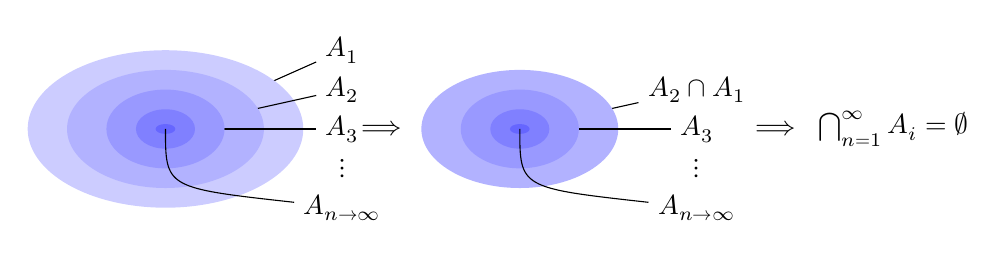
\begin{tikzpicture}[scale=0.5]
    \def\one{(4.5,2.5) ellipse (3.5 cm and 2 cm)};
    \def\two{(4.5,2.5) ellipse (2.5 cm and 1.5 cm)};
    \def\three{(4.5,2.5) ellipse (1.5 cm and 1 cm)};
    \def\four{(4.5,2.5) ellipse (0.75 cm and 0.5 cm)};
    \def\five{(4.5,2.5) ellipse (0.25 cm and 0.125 cm)};
    \node (n1) at (9,4.5) {$A_{1}$};
    \draw (4.5,2.5) -- (n1);
    \fill[fill=blue!20]\one;
    \node (n2) at (9,3.5) {$A_{2}$};
    \draw (4.5,2.5) -- (n2);
    \fill[fill=blue!30]\two;
    \node (n3) at (9,2.5) {$A_{3}$};
    \draw (4.5,2.5) -- (n3);
    \fill[fill=blue!40]\three;
    \fill[fill=blue!50]\four;
    \fill[fill=blue!60]\five;
    \node (n4) at (9,1.5) {$\vdots$};
    \node (nn) at (9,0.5) {$A_{n\to \infty}$};
    \draw (4.5,2.5) .. controls +(down:1.5cm) .. (nn);
    \node (meioum) at (10,2.5) {$\Longrightarrow$};
    \def\twoz{(13.5,2.5) ellipse (2.5 cm and 1.5 cm)};
    \def\threez{(13.5,2.5) ellipse (1.5 cm and 1 cm)};
    \def\fourz{(13.5,2.5) ellipse (0.75 cm and 0.5 cm)};
    \def\fivez{(13.5,2.5) ellipse (0.25 cm and 0.125 cm)};
    \node (n22) at (18,3.5) {$A_{2} \cap A_{1}$};
    \draw (13.5,2.5) -- (n22);
    \fill[fill=blue!30]\twoz;
    \node (n32) at (18,2.5) {$A_{3}$};
    \draw (13.5,2.5) -- (n32);
    \fill[fill=blue!40]\threez;
    \fill[fill=blue!50]\fourz;
    \fill[fill=blue!60]\fivez;
    \node (n42) at (18,1.5) {$\vdots$};
    \node (nn2) at (18,0.5) {$A_{n \to \infty}$};
    \draw (13.5,2.5) .. controls +(down:1.5cm) .. (nn2);
    \node (meiodois) at (20,2.5) {$\Longrightarrow$};
    \node (final) at (23,2.5) {$\bigcap_{n=1}^{\infty}A_{i} = \emptyset$};
\end{tikzpicture}
\end{center}

\begin{proposition}
\protect\hypertarget{prp:axiomas}{}\label{prp:axiomas}Dados os axiomas \(Ax_{1}(K),Ax_{2}(K),Ax_{3}(K)\), o axioma 4 é equivalente ao axioma \(Ax'_{3}(K)\), ou seja, uma probabilidade finitamente aditiva é uma medida de probabilidade se e somente se é contínua no vazio.
\end{proposition}

A prova de que a \(\sigma\)-aditividade implica o axioma 4 é consequência da prova da proposição anterior, dado que \(\bigcap_{n=1}^{\infty}A_{n} = \emptyset\). Para demonstrar o contrário (que \(Ax_{1}(K) + Ax_{2}(K) + Ax_{3}(K) + Ax_{4}(K) \rightarrow Ax'_{3}(K)\)), tomemos uma sequência infinita de eventos \(\{A_{i}\}_{i \ge 1}\) em \(\mathcal{A} : A_{i} \cap A_{j} = \emptyset \; \forall i \neq j\). Devemos ver que \(P(\bigcup_{n=1}^{\infty}) = \sum_{n=1}^{\infty}P(A_{n})\). Seja \(A = \bigcup_{n=1}^{\infty}A_{n} = (\bigcup_{n=1}^{k}A_{n}) \cup (\bigcup_{n=k+1}^{\infty}A_{n})\). Tem-se que:

\begin{equation*}
P(A) = P\left(\bigcup_{n=1}^{k}A_{n}\right) + P\left(\bigcup_{n=k+1}^{\infty}A_{n}\right) = \sum_{n=1}^{k}P(A_{n}) +P\left(\bigcup_{n=k+1}^{\infty}A_{n}\right)
\end{equation*}

Seja \(B_{k} = \bigcup_{n=k+1}^{\infty}A_{n}\). Note que \(B_{k} \downarrow \emptyset\) quando \(k \to \infty\) de modo que \(P(B_{k})\xrightarrow[k \to \infty]{}0\), logo:

\begin{equation*}
\lim_{k \to \infty}\sum_{n=1}^{k}P(A_{n}) = \sum_{n=1}^{\infty}P(A_{n})
\end{equation*}

\begin{corollary}
Os seguintes sistemas são equivalentes:

\begin{equation*}
Ax_{1}(K),Ax_{2}(K),Ax'_{3}(K) \equiv Ax_{1}(K),Ax_{2}(K),Ax_{3}(K),Ax_{4}(K)
\end{equation*}
\end{corollary}

\hypertarget{propriedades-de-probabilidade}{%
\subsection{Propriedades de probabilidade}\label{propriedades-de-probabilidade}}

Seja \(P\) uma probabilidade em uma \(\sigma\)-álgebra \(\mathcal{A}\). Suponhamos que todo \(A\) abaixo pertença à \(\mathcal{A}\). Então as seguintes propriedades são consequências dos axiomas:

\begin{itemize}
\tightlist
\item
  \textbf{P1}: \(P(A^{c}) = 1 - P(A)\);
\item
  \textbf{P2}: \(0 \le P(A) \le 1\);
\item
  \textbf{P3}: \(A_{1} \subset A_{2} \Rightarrow P(A_{1}) \le P(A_{2})\);
\item
  \textbf{P4}: \(P(\bigcup_{i=1}^{n}A_{i}) \le \sum_{i=1}^{n}P(A_{i})\);
\item
  \textbf{P5}: \(P(\bigcup_{i=1}^{\infty}A_{i}) \le \sum_{i=1}^{\infty}P(A_{i})\);
\end{itemize}

Com essas propriedades, podemos então definir um modelo probabilístico. Sejam:

\begin{itemize}
\tightlist
\item
  \textbf{a}) Um espaço amostral: \(\Omega \neq \emptyset\);
\item
  \textbf{b}) Uma \(\sigma\)-álgebra em \(\Omega\): \(\mathcal{A}\);
\item
  \textbf{c}) Uma medida de probabilidade em \(\mathcal{A}\): \(P\).
\end{itemize}

\begin{definition}
Um espaço de probabilidade é uma terna \((\Omega,\mathcal{A},P)\) seguindo \textbf{a},\textbf{b} e \textbf{c}.
\end{definition}

\hypertarget{probabilidade-condicional-e-independuxeancia}{%
\subsection{Probabilidade Condicional e Independência}\label{probabilidade-condicional-e-independuxeancia}}

Considere o seguinte experimento: um dado é lançado duas vezes e anota-se a dupla de resultados. Temos que:

\begin{equation*}
\Omega = \{(i,j) : 1 \le i \le 6; 1 \le j \le 6; i,j, \in \mathbb{Z}\}
\end{equation*}

Sejam os seguintes eventos:

\begin{itemize}
\tightlist
\item
  \(A = "\textit{em cada lançamento o valor observado é } \le 2"\);
\item
  \(B = "\textit{a soma dos resultados é igual a 4}"\).
\end{itemize}

\begin{align*}
A &= \{(1,1),(1,2),(2,1),(2,2)\} \\
B &= \{(1,3),(3,1),(2,2)\}
\end{align*}

Já que \(\#\Omega = |\Omega| = 36\), e pela equiprobabilidade dos eventos (considerando que os dados são honestos), temos que:

\begin{align*}
P(A) &= \frac{|A|}{|\Omega|} = \frac{4}{36} \\
P(B) &= \frac{|B|}{|\Omega|} = \frac{3}{36}
\end{align*}

Além disso, \((A \cap B) = \{(2,2)\}; P(A \cap B) = 1/36\). Suponha que \(A\) ocorre com \(P(A) > 0\), e que \(B\) é o evento de interesse. Assumindo a potencial ocorrência de \(A\), qual é a probabilidade de \(B\) ocorrer. Nesse caso \(P(B|A) = 1/4\).

\begin{definition}[Probabilidade condicional]
Sejam \(A\) e \(B\) eventos em \(\mathcal{A}\), com \(P(A) > 0\). A probabilidade condicional \(P(B|A)\) é definida como:

\begin{equation}
P(B|A) = \frac{P(A \cap B)}{P(A)}
\label{eq:probcond}
\end{equation}

ou equivalentemente:

\begin{equation}
P(A \cap B) = P(B|A)P(A)
\label{eq:probconddif}
\end{equation}
\end{definition}

\begin{example}

Considere uma urna com 5 bolas, sendo 3 vermelhas e 2 brancas. O experimento consiste de 2 retiradas sucessivas de uma bola da urna (sem reposição). Considere os eventos \(A_{1} = \textit{Cor da primeira bola}\) e \(A_{2} = \textit{Cor da segunda bola}\):

\begin{align*}
P(A_{1} = B) = \frac{2}{5} \;&,\; P(A_{1} = V) = \frac{3}{5} \\
P(A_{2} = B|A_{1} = B) = \frac{1}{4} \;&,\; P(A_{2} = V|A_{1} = B) = \frac{3}{4} \\
P(A_{2} = B|A_{1} = V) = \frac{2}{4} \;&,\; P(A_{2} = V|A_{1} = V) = \frac{2}{4}
\end{align*}

Podemos visualizar esse experimento com os seguintes diagrama e tabela de probabilidades:

\begin{center}
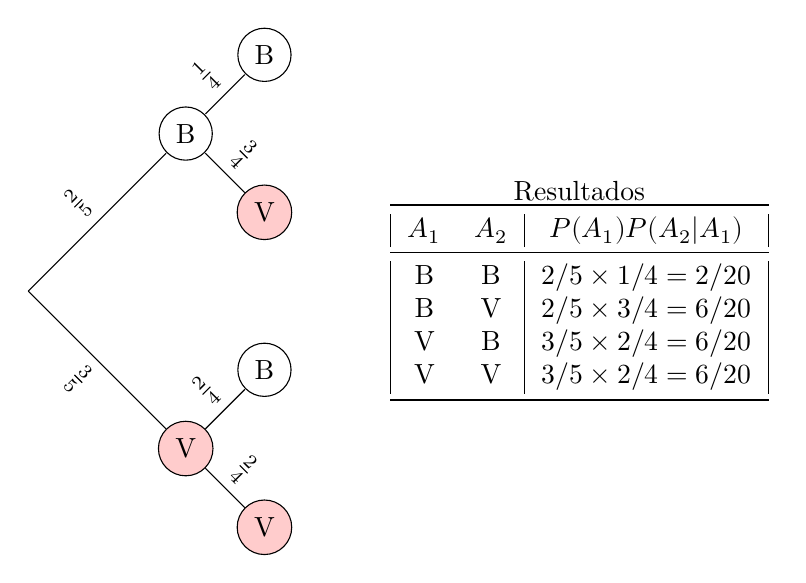
\begin{tikzpicture}
    \draw (0,0) -- (1.75,1.75) node[midway,sloped,above] {$\frac{2}{5}$};
    \draw (2,2) node[circle,draw] {B};
    \draw (2.25,2.25) -- (2.75,2.75) node[midway,sloped,above] {$\frac{1}{4}$};
    \draw (3,3) node[circle,draw] {B};
    \draw (2.25,1.75) -- (2.75,1.25) node[midway,sloped,above] {$\frac{3}{4}$};
    \draw (3,1) node[circle,draw,fill=red!20] {V};
    \draw (0,0) -- (1.75,-1.75) node[midway,sloped,below] {$\frac{3}{5}$};
    \draw (2,-2) node[circle,draw,fill=red!20] {V};
    \draw (2.25,-2.25) -- (2.75,-2.75) node[midway,sloped,above] {$\frac{2}{4}$};
    \draw (3,-1) node[circle,draw] {B};
    \draw (2.25,-1.75) -- (2.75,-1.25) node[midway,sloped,above] {$\frac{2}{4}$};
    \draw (3,-3) node[circle,draw,fill=red!20] {V};
    \node [shape=rectangle, align=center](table1) at (7,0) {
        Resultados \\
        \begin{tabular}{|cc|c|} \toprule
        $A_{1}$ & $A_{2}$  & $P(A_{1})P(A_{2}|A_{1})$ \\ \midrule
        B & B & $2/5 \times 1/4 = 2/20$ \\
        B & V & $2/5 \times 3/4 = 6/20$ \\
        V & B & $3/5 \times 2/4 = 6/20$ \\
        V & V & $3/5 \times 2/4 = 6/20$ \\ \bottomrule
        \end{tabular}
    };
\end{tikzpicture}
\end{center}

\end{example}

\begin{definition}[Eventos independentes]
\leavevmode

\begin{itemize}
\tightlist
\item
  \textbf{a}) Os eventos \(A\) e \(B\) são independentes (denotados como \(A \perp B\)) se \(P(A \cap B) = P(A)P(B)\);
\item
  \textbf{b}) \(\{A_{i}, i \in \mathbb{I}\}\) são independentes se \(P\left(\bigcap_{i \in \mathcal{J}}A_{i}\right) = \prod_{i \in \mathcal{J}}P(A_{i}), \; \forall\text{ subfamílias } \mathcal{J} \text{ de índices em } \mathbb{I}\).
\end{itemize}

\end{definition}

Disso segue que, sendo \(A\) e \(B\) dois eventos, as seguintes propriedades são válidas:

\begin{enumerate}
\def\labelenumi{\arabic{enumi}.}
\tightlist
\item
  Se \(P(A) = 0 \Rightarrow P(A \cap B) = 0 \; \forall B\), ou seja, \(A \perp B\);
\item
  Se \(P(B) = 1 \Rightarrow P(A \cap B) = 0 \; \forall A\), ou seja, \(A \perp B\);
\item
  \(A\) é independente dele mesmo se e somente se \(P(A) = 0\) ou \(P(A) = 1\);
\item
  \(A \perp B \Rightarrow A \perp B^{c}, A^{c} \perp B, A^{c} \perp B^{c}\);
\item
  As seguintes proposições são equivalentes:

  \begin{itemize}
  \item
    \begin{enumerate}
    \def\labelenumii{\alph{enumii})}
    \tightlist
    \item
      \((A \perp B) \Rightarrow P(B|A) = P(B)\) e \(P(B|A^{c}) = P(B)\);
    \end{enumerate}
  \item
    \begin{enumerate}
    \def\labelenumii{\alph{enumii})}
    \setcounter{enumii}{1}
    \tightlist
    \item
      \(P(B|A) = P(B) \Rightarrow A \perp B\);
    \end{enumerate}
  \item
    \begin{enumerate}
    \def\labelenumii{\alph{enumii})}
    \setcounter{enumii}{2}
    \tightlist
    \item
      \(P(B|A^{c}) = P(B) \Rightarrow A \perp B\).
    \end{enumerate}
  \end{itemize}
\end{enumerate}

\begin{theorem}[Teorema das Probabilidades Totais]
\leavevmode

\begin{enumerate}
\def\labelenumi{\arabic{enumi}.}
\tightlist
\item
  Dados \(A\) e \(B\) eventos em \(\mathcal{F}\):
\end{enumerate}

\begin{equation*}
P(A) = P(A|B)P(B) + P(A|B^{c})P(B^{c})
\end{equation*}

\begin{enumerate}
\def\labelenumi{\arabic{enumi}.}
\setcounter{enumi}{1}
\tightlist
\item
  No geral, se \(B_{1},B_{2}, \ldots, B_{n}\) é uma partição de \(\Omega\), então:
\end{enumerate}

\begin{equation}
P(A) = \sum_{i=1}^{n}P(A|B_{i})P(B_{i})
\label{eq:teorprobtotal}
\end{equation}

\end{theorem}

\textbf{Demonstração}: Note que \(A = (A \cap B) \cup (A \cap B^{c})\) e \((B \cap B^{c}) = \emptyset\) e \((B \cup B^{c}) = \Omega\). Além disso, \((A \cap B) \cap (A \cap B^{c}) = \emptyset\), logo \(P(A) = P(A \cap B) + P(A \cap B^{c})\). Como, por definição, \(P(A|B) = P(A \cap B) / P(B)\) e \(P(A|B^{c}) = P(A \cap B^{c}) / P(B^{c})\), temos que:

\begin{equation*}
P(A) = P(A|B)P(B) + P(A|B^{c})P(B^{c})
\end{equation*}

Para o caso geral, temos que \(\{B_{i}\}_{i=1}^{n} , \; (B_{i} \cap B_{j}) = \emptyset \; \forall i,j\) e \(\bigcup_{i=1}^{n}B_{i} = \Omega\). Logo:

\begin{align*}
A &= (A \cap B_{1}) \cup (A \cap B_{2}) \cup \ldots \cup (A \cap B_{n}) \\
&\Downarrow \; \text{Pela }\sigma\text{-aditividade} \\
P(A) &= \sum_{i=1}^{n}P(A \cap B_{i})
\end{align*}

E como \(P(A|B_{i}) = P(A \cap B_{i}) \ P(B_{i})\):

\begin{equation*}
P(A) = \sum_{i=1}^{n}P(A|B_{i})P(B_{i})
\end{equation*}

\hypertarget{fuxf3rmula-de-poincaruxe9-e-teorema-de-bayes}{%
\subsection{Fórmula de Poincaré e Teorema de Bayes}\label{fuxf3rmula-de-poincaruxe9-e-teorema-de-bayes}}

\begin{theorem}[Fórmula de Poincaré]
Seja \(\{A_{i}\}_{i \ge 1} \subseteq \mathcal{F}\). Então:

\begin{equation}
\begin{split}
P\left(\bigcup_{i=1}^{n} A_{n}\right) = &\sum_{i=1}^{n}P(A_{i}) - \sum_{1 \le i_{1} < i_{2} \le n} P(A_{i_{1}} \cap A_{i_{2}}) + \sum_{1 \le i_{1} < i_{2} < i_{3} \le n} P(A_{i_{1}} \cap A_{i_{2}} \cap A_{i_{3}}) - \dots \\
&+ (-1)^{n+1} P(A_{1} \cap A_{2} \cap \ldots \cap A_{n})
\label{eq:formulapoincare}
\end{split}
\end{equation}
\end{theorem}

A demonstração da fórmula \eqref{eq:formulapoincare} é dada no exercício \ref{exr:exbj13}.

\begin{theorem}[Teorema de Bayes]
Seja \(\{B_{i}\}_{i=1}^{n}\) uma partição de \(\Omega\) e \(A\) um evento em \(\mathcal{F}\), temos que:

\begin{equation}
P(B_{i}|A) = \frac{P(A|B_{i})P(B_{i})}{\sum_{j=1}^{n}P(A|B_{j})P(B_{j})}
\label{eq:teoremabayes}
\end{equation}
\end{theorem}

O denominador de \eqref{eq:teoremabayes} é derivado do teorema das probabilidades totais, visto que \(\{B_{i}\}_{i=1}^{n}\) é uma partição de \(\Omega\).

\begin{lemma}
Sejam \(A_{1},A_{2}, \ldots, A_{n}\) eventos em \(\mathcal{F}\), logo:

\begin{equation*}
P\left(\bigcap_{i=1}^{n}A_{i}\right) = P(A_{1})P(A_{2}|A_{1})P(A_{3}|A_{1} \cap A_{2}) \ldots P(A_{n}|A_{1} \cap A_{2} \cap \ldots \cap A_{n-1})
\end{equation*}
\end{lemma}

\begin{proof}[Prova]
Suponha a validade do lema anterior. Logo, seja \(D = (\bigcap_{i=1}^{n}A_{i})\):

\begin{align*}
P(A_{1} \cap \ldots \cap A_{n} \cap A_{n+1}) &= P(D \cap A_{n+1}) \\
&= P(D)P(A_{n+1}|D) \\
&= P(A_{1})P(A_{2}|A_{1}) \ldots P(A_{n}|A_{1} \cap \ldots \cap A_{n-1})P(A_{n+1}|A_{1} \cap \ldots \cap A_{n})
\end{align*}
\end{proof}

\newpage

\hypertarget{exercuxedcios}{%
\subsection{Exercícios}\label{exercuxedcios}}

\begin{exercise}[BJ1]

Sejam \(A, B\) e \(C\) eventos aleatórios. Identifique as seguintes equações e frases, casando cada equação expressa na notação de conjuntos com a correspondente frase na linguagem de eventos:

\begin{center}
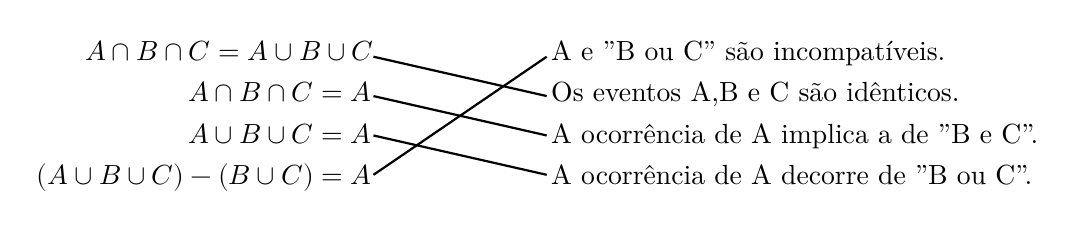
\begin{tikzpicture}
    \node (a) at (0,0) {$
        \begin{aligned}
            A \cap B \cap C = A \cup B \cup C &\\
            A \cap B \cap C = A &\\
            A \cup B \cup C = A &\\
            (A \cup B \cup C) - (B \cup C) = A &
        \end{aligned}$};
    \node (i) at (7.5,0) {$
        \begin{aligned}
            & \text{A e "B ou C" são incompatíveis.}\\
            & \text{Os eventos A,B e C são idênticos.}\\
            & \text{A ocorrência de A implica a de "B e C".}\\
            & \text{A ocorrência de A decorre de "B ou C".}
        \end{aligned}
    $};
    \draw[thick] (2.15,0.75) -- (4.35,0.25);
    \draw[thick] (2.15,0.25) -- (4.35,-0.25);
    \draw[thick] (2.15,-0.25) -- (4.35,-0.75);
    \draw[thick] (2.15,-0.75) -- (4.35,0.75);
\end{tikzpicture}
\end{center}

\end{exercise}

\begin{exercise}[BJ2]
\protect\hypertarget{exr:exbj2}{}\label{exr:exbj2}

A partir dos axiomas, prove a propriedade \(P5\):

\[
P\left(\bigcup_{n=i}^{\infty}A_{n}\right) \le \sum_{n=1}^{\infty}P(A_{n})
\]

\begin{proof}[Resposta]
Consideremos uma prova por indução para \(n \to \infty\):

Para \(n=2\):

\[
P(A_{1} \cup A_{2}) = P(A_{1}) + P(A_{1}^{c} \cap A_{2})
\]

Considerando que \((A_1^{c} \cap A_{2}) \subset A_{2}\) e o fato de que \((A_{1}) \cap (A_{1}^{c} \cap A_{2}) = \emptyset\), temos pela propriedade \(P3\) que \(P(A_1^{c} \cap A_{2}) \le P(A_{2})\), de modo que:

\begin{align*}
P(A_{1} \cup A_{2}) &= P(A_{1}) + P(A_{1}^{c} \cap A_{2}) \le P(A_{2}) \\
&\le P(A_{1}) + P(A_{2})\\
&\le \sum_{i=1}^{2}P(A_{i})
\end{align*}

De modo semelhante, podemos fazer para \(n\):

\begin{align*}
P\left(\bigcup_{i=i}^{n}A_{i}\right) &= P(A_{1}) + P(A_{1}^{c} \cap A_{2}) + \dots \\
&\le P(A_{1}) + P(A_{2}) + \dots\\
&\le \sum_{i=1}^{n}P(A_{i})
\end{align*}

Consideremos então uma sequência de eventos \(A_{i}^{*},\forall i \in \{n+1,n+2,\dots\}\), disjuntos de \(A_{i}\). Denotemos ainda \(A = \left(\bigcup_{i = 1}^{n}A_{i}\right) \cup \left(\bigcup_{i=n+1}^{\infty}A_{i}\right)\). Pela aditividade infinita (ou ainda pela \(\sigma\)-aditividade), temos que:

\[
P\left(\bigcup_{n=i}^{\infty}A_{n}\right) \le \sum_{i=1}^{n}P(A_{i}) + P\left(\bigcup_{i=n+1}^{\infty}A_{i}\right)
\]

Que por serem disjuntos, pelo axioma \(Ax_{4}\) tem que \(\left(\bigcup_{i=n+1}^{\infty}A_{i}\right)\downarrow \emptyset\), de modo que \(P\left(\bigcup_{i=n+1}^{\infty}A_{i}\right) \to 0\). Logo, tem-se que:

\[
P\left(\bigcup_{n=i}^{\infty}A_{n}\right) \le \sum_{n=1}^{\infty}P(A_{n})
\]
\end{proof}

\end{exercise}

\begin{exercise}[BJ3]
\protect\hypertarget{exr:exbj3}{}\label{exr:exbj3}

Sejam \(A_{1}, A_{2},\dots\) eventos aleatórios. Mostre que:

\begin{enumerate}
\def\labelenumi{\alph{enumi})}
\tightlist
\item
  \(P\left(\bigcap_{k=1}^{n}A_{k}\right) \ge 1 - \sum_{k=1}^{n}P(A_{k}^{c})\)
\end{enumerate}

\begin{proof}[Resposta]
Por De Morgan temos que \(\bigcap_{k=1}^{n}A_{k} = \left(\bigcup_{k=1}^{n}A_{k}^{c}\right)^{c}\), de modo que:

\begin{align*}
P\left(\bigcap_{k=1}^{n}A_{k}\right) &= P\left(\bigcup_{k=1}^{n}A_{k}^{c}\right)^{c} \\
&= 1 - P\left(\bigcup_{k=1}^{n}A_{k}^{c}\right) \xRightarrow[]{\text{Por P4}} P\left(\bigcup_{k=1}^{n}A_{k}^{c}\right) \le \sum_{k=1}^{n}P\left(A_{k}^{c}\right) \\
&\ge 1 - \sum_{k=1}^{n}P\left(A_{k}^{c}\right)
\end{align*}
\end{proof}

\begin{enumerate}
\def\labelenumi{\alph{enumi})}
\setcounter{enumi}{1}
\tightlist
\item
  Se \(P(A_{k}) \ge 1 - \epsilon\) para \(k = 1,2,\dots,n\), então \(P(\bigcap_{k=1}^{n}A_{k}) \ge 1 - n\epsilon\)
\end{enumerate}

\begin{proof}[Resposta]
É fácil ver que:

\[
P(A_{k}) \ge 1 - \epsilon \Rightarrow P(A_{k}^{c}) \le 1 - (1-\epsilon) = \epsilon
\]

E de modo semelhante ao que foi feito na questão anterior (utilizando De Morgan), temos que:

\begin{align*}
P\left(\bigcap_{k=1}^{n}A_{k}\right) = P\left(\bigcup_{k=1}^{n}A_{k}^{c}\right)^{c} &= 1 - P\left(\bigcup_{k=1}^{n}A_{k}^{c}\right)\\
&\ge 1 - \sum_{k=1}^{n}P\left(A_{k}^{c}\right) \\
&\ge 1 - \sum_{k=1}^{n}\epsilon\\
&\ge 1 - n\epsilon
\end{align*}
\end{proof}

\begin{enumerate}
\def\labelenumi{\alph{enumi})}
\setcounter{enumi}{2}
\tightlist
\item
  \(P\left(\bigcap_{k=1}^{\infty}A_{k}\right) \ge 1 - \sum_{k=1}^{\infty}P(A_{k}^{c})\)
\end{enumerate}

\begin{proof}[Resposta]
De maneira semelhante ao que foi visto na prova da letra \textbf{a}, temos que:

\begin{align*}
P\left(\bigcap_{k=1}^{\infty}A_{k}\right) &= P\left(\bigcup_{k=1}^{\infty}A_{k}^{c}\right)^{c} \\
&= 1 - P\left(\bigcup_{k=1}^{\infty}A_{k}^{c}\right) \xRightarrow[]{\text{Por P5}} P\left(\bigcup_{k=1}^{n}A_{k}^{c}\right) \le \sum_{k=1}^{\infty}P\left(A_{k}^{c}\right) \\
&\ge 1 - \sum_{k=1}^{\infty}P\left(A_{k}^{c}\right)
\end{align*}

Para ver a demonstração da propriedade \(P5\), vide exercício \ref{exr:exbj2}.
\end{proof}

\end{exercise}

\begin{exercise}[BJ4]

Demonstre as seguintes propriedades:

\begin{enumerate}
\def\labelenumi{\alph{enumi})}
\tightlist
\item
  Se \(P(A_{n}) = 0\) para \(n = 1,2,\dots\), então \(P\left(\bigcup_{n=1}^{\infty}A_{n}\right) = 0\).
\end{enumerate}

\begin{proof}[Resposta]
Utilizando a propriedade \(P5\), temos que:

\begin{align*}
P\left(\bigcup_{n=1}^{\infty} A_{n}\right) &\le \sum_{n=1}^{\infty}P(A_{n}) \\
&\le \sum_{n=1}^{\infty}0 \\
&\le 0 \\
&\;\Big\downarrow \;\text{Por } P2\\
P\left(\bigcup_{n=1}^{\infty} A_{n}\right) &= 0
\end{align*}
\end{proof}

\begin{enumerate}
\def\labelenumi{\alph{enumi})}
\setcounter{enumi}{1}
\tightlist
\item
  Se \(P(A_{n}) = 1\) para \(n = 1,2,\dots\), então \(P\left(\bigcap_{n=1}^{\infty}A_{n}\right) = 1\).
\end{enumerate}

\begin{proof}[Resposta]
Levando em consideração que se \(P(A_{n}) = 1 \Rightarrow P(A_{n}^{c}) = 0\) (pela propriedade \(P1\)), utilizando De Morgan e a prova da letra \textbf{c} do exercício \ref{exr:exbj3}, temos que:

\begin{align*}
P\left(\bigcap_{n=1}^{\infty}A_{n}\right) &\ge 1 - \sum_{n=1}^{\infty} P(A_{n}^{c}) \\
&\ge 1 - \sum_{n=1}^{\infty}0 \\
&\ge 1 - 0 \\
&\ge 1 \\
&\;\Big\downarrow \;\text{Por } P2\\
P\left(\bigcap_{n=1}^{\infty}A_{n}\right) &= 1
\end{align*}
\end{proof}

\end{exercise}

\begin{exercise}[BJ6]

Seja \(\Omega\) um conjunto não-vazio.

\begin{enumerate}
\def\labelenumi{\alph{enumi})}
\tightlist
\item
  Prove: se \(\mathcal{A}\) e \(\mathcal{B}\) são \(\sigma\)-álgebras de subconjuntos de \(\Omega\), então \((\mathcal{A} \cap \mathcal{B})\) também é uma \(\sigma\)-álgebra.
\end{enumerate}

\begin{proof}[Resposta]
Para que \(\mathcal{A} \cap \mathcal{B}\) seja uma \(\sigma\)-álgebra, é necessário que cumpram-se os axiomas \(Ax_{1}, Ax_{2}\) e \(Ax_{3}\):

\begin{itemize}
\tightlist
\item
  \(Ax_{1}\): Sabemos que \(\Omega \in \mathcal{A}\) e \(\Omega \in \mathcal{B}\), logo sabemos que \(\Omega \in (\mathcal{A} \cap \mathcal{B})\);
\item
  \(Ax_{2}\): Seja um evento \(E \in (\mathcal{A} \cap \mathcal{B})\), sabemos então que \(E \in \mathcal{A}\) e \(E \in \mathcal{B}\), logo \(E^{c} \in \mathcal{A}\) e \(E^{c} \in \mathcal{B}\), portanto \(E^{c} \in (\mathcal{A} \cap \mathcal{B})\);
\item
  \(Ax_{3}\): Sejam dois eventos, \(E_{1} \in (\mathcal{A} \cap \mathcal{B})\) e \(E_{2} \in (\mathcal{A} \cap \mathcal{B})\). Com isso, temos que \(E_{1}, E_{2} \in \mathcal{A}\) e \(E_{1}, E_{2} \in \mathcal{B}\), portanto \((E_{1} \cup E_{2}) \in \mathcal{A}\) e \(E_{1} \cup E_{2} \in \mathcal{B}\), logo \((E_{1} \cup E_{2}) \in (\mathcal{A} \cap \mathcal{B})\).
\end{itemize}

Como os três axiomas foram cumpridos, temos que \((\mathcal{A} \cap \mathcal{B})\) é uma \(\sigma\)-álgebra.
\end{proof}

\begin{enumerate}
\def\labelenumi{\alph{enumi})}
\setcounter{enumi}{1}
\tightlist
\item
  Generalize o item (a): se \(\mathcal{A}_{i}, i \in \mathcal{I}\), são \(\sigma\)-álgebras de partes de \(\Omega\), onde \(\mathcal{I}\) é um conjunto não-vazio de índices, então \(\bigcap_{i \in \mathcal{I}}\mathcal{A}_{i}\) também é uma \(\sigma\)-álgebra.
\end{enumerate}

\begin{proof}[Resposta]
Como anteriormente, temos que mostrar que \(\bigcap_{i \in \mathcal{I}}\mathcal{A}_{i}\) cumpre os axiomas \(Ax_{1}, Ax_{2}\) e \(Ax_{3}\):

\begin{itemize}
\tightlist
\item
  \(Ax_{1}\): Sabemos que \(\Omega \in \mathcal{A}_{i}, \; \forall i \in \mathcal{I}\), logo sabemos que \(\Omega \in \bigcap_{i \in \mathcal{I}}\mathcal{A}_{i}\);
\item
  \(Ax_{2}\): Seja um evento \(E \in \bigcap_{i \in \mathcal{I}}\mathcal{A}_{i}\), sabemos então que \(E \in \mathcal{A}_{i}, \; \forall i \in \mathcal{I}\), logo \(E^{c} \in \mathcal{A}_{i}, \; \forall i \in \mathcal{A}\), portanto \(E^{c} \in \bigcap_{i \in \mathcal{I}}\mathcal{A}_{i}\);
\item
  \(Ax_{3}\): Sejam dois eventos, \(E_{1} \in \bigcap_{i \in \mathcal{I}}\mathcal{A}_{i}\) e \(E_{2} \in \bigcap_{i \in \mathcal{I}}\mathcal{A}_{i}\). Com isso, temos que \(E_{1}, E_{2} \in \mathcal{A}_{i}, \; \forall i \in \mathcal{I}\), portanto \((E_{1} \cup E_{2}) \in \mathcal{A}_{i}, \; \forall i \in \mathcal{I}\), logo \((E_{1} \cup E_{2}) \in \bigcap_{i \in \mathcal{I}}\mathcal{A}_{i}\).
\end{itemize}

Vemos portanto que, por cumprir os axiomas \(Ax_{1}, Ax_{2}\) e \(Ax_{3}\), \(\bigcap_{i \in \mathcal{I}}\mathcal{A}_{i}\) é também uma \(\sigma\)-álgebra.
\end{proof}

\begin{enumerate}
\def\labelenumi{\alph{enumi})}
\setcounter{enumi}{2}
\tightlist
\item
  Seja \(\mathbb{C}\) uma classe de subconjuntos de \(\Omega\). Mostre que existe \emph{pelo menos uma} \(\sigma\)-álgebra que contém \(\mathbb{C}\).
\end{enumerate}

\begin{proof}[Resposta]
É fácil ver que a maior classe de subconjuntos de \(\Omega\) é o conjunto das partes de \(\Omega\), denotado como \(\mathcal{P}(\Omega)\) (definido no exemplo \ref{exm:powerset}). Assim, temos que \(\mathbb{C} \subseteq \mathcal{P}(\Omega)\), de modo que, pelo menos a \(\sigma\)-álgebra formada por \(\mathcal{P}(\Omega)\) contém \(\mathbb{C}\).
\end{proof}

\begin{enumerate}
\def\labelenumi{\alph{enumi})}
\setcounter{enumi}{3}
\tightlist
\item
  Visando a plena utilização dos itens (b) e (c), como você definiria ``a menor \(\sigma\)-álgebra contendo \(\mathbb{C}\)'', onde \(\mathcal{C}\) é uma classe de subconjuntos de \(\Omega\)?
\end{enumerate}

\begin{proof}[Resposta]
Considere que temos \(\sigma\)-álgebras de partes de \(\Omega\), \(\mathcal{A}_{i}\) com \(i \in \mathbb{I}\) (sendo \(\mathbb{I}\) um conjunto não-vazio de índices), tais que \(\mathbb{C} \in \mathcal{A}_{i}: \; \forall i \in \mathbb{I}\). Assim, sabemos que algum dos \(\mathcal{A}_{i}\) é a menor \(\sigma\)-álgebra que contém \(\mathbb{C}\), de modo que \(\bigcap_{i \in \mathbb{I}}A_{i}\) será a menor \(\sigma\)-álgebra que contém \(\mathbb{C}\).
\end{proof}

\end{exercise}

\begin{exercise}[BJ9]

Uma caixa contém \(2n\) sorvetes, \(n\) do sabor \(A\) e \(n\) do sabor \(B\). De um grupo de \(2n\) pessoas, \(a < n\) preferem o sabor \(A\), \(b < n\) o sabor \(B\) e \(2n-(a+b)\) não tem preferência. Demonstre: se os sorvetes são distribuídos ao acaso, a probabilidade de que a preferência de todas as pessoas seja respeitada é de \(\binom{2n-a-b}{n-a}/\binom{2n}{n}\).

\begin{proof}[Resposta]
Sabendo que a ordem de entrega dos \(n\) sorvetes de cada sabor, para as \(2n\) pessoas não importa, temos que a quantidade possível de entregas diferentes é:

\begin{equation*}
|\Omega| = \binom{2n}{n}
\end{equation*}

Considere que o evento \(R\) indica o caso em que todos tiveram sua preferência respeitada. Podemos ver que:

\begin{equation*}
P(R) = \frac{|R|}{|\Omega|} = \frac{|R|}{\binom{2n}{n}}
\end{equation*}

Para que \(R\) ocorra, é necessário que as \(a\) pessoas que preferem \(A\) recebam esse sabor, bem como as \(b\) pessoas que preferem \(B\). Dessa forma, temos que distribuir os \(2n-(a+b)\) sorvetes restantes para as pessoas que não tem preferência. Assim, primeiramente temos os \(n-a\) sorvetes do sabor \(A\) que não foram alocados, de forma que:

\begin{equation}
\binom{2n-a-b}{n-a} = \frac{(2n-a-b)!}{(2n-a-b-n+a)!(n-a)!} = \frac{(2n-a-b)!}{(n-b)!(n-a)!}\\
\label{eq:aloca}
\end{equation}

E podemos mostrar que, caso fossemos alocar os \(n-b\) sorvetes do sabor \(B\) para as \(2n-(a+b)\) pessoas sem preferência, teríamos:

\begin{equation}
\binom{2n-a-b}{n-b} = \frac{(2n-a-b)!}{(2n-a-b-n+b)!(n-b)!} = \frac{(2n-a-b)!}{(n-a)!(n-b)!}\\
\label{eq:alocb}
\end{equation}

Como \eqref{eq:aloca} e \eqref{eq:aloca} são iguais, podemos ver que a alocação dos sorvetes restantes não depende de qual sabor já foi alocado. Assim, temos que \(|R| = \binom{2n-a-b}{n-a} = \binom{2n-a-b}{n-b}\), portanto:

\begin{equation*}
P(R) = \frac{|R|}{|\Omega|} = \frac{\binom{2n-a-b}{n-a}}{\binom{2n}{n}}
\end{equation*}
\end{proof}

\end{exercise}

\begin{exercise}[BJ10]

Suponhamos que dez cartas estejam numeradas de 1 até 10. Das dez cartas, retira-se uma de cada vez, ao acaso e sem reposição, até retirar-se o primeiro número par. Conta-se o número de retiradas necessárias. Exiba um bom modelo probabilístico para esse experimento.

\begin{proof}[Resposta]
Dada essa formulação, temos que 5 cartas são pares e 5 são ímpares. Assim, considere o evento \(\{Y_{k} \;: 1 \le k \le 6 ; k \in \mathbb{Z}\}\) em que \(k\) indica que a \(k\)-ésima retirada contém a primeira carta par. Assim, por exemplo, \(Y_{1}\) indica o evento em que a primeira carta retirada é par, \(Y_{2}\) o evento em que a segunda carta retirada é par, e assim por diante.

O nosso espaço amostral é (visto que o número da carta não importa, apenas se é \(P = "\text{par}"\) ou \(I = "\text{ímpar}"\)):

\begin{equation*}
\Omega = \{(P), (I,P), (I,I,P), (I,I,I,P), (I,I,I,I,P), (I,I,I,I,I,P)\}\\
\end{equation*}

É fácil ver que não é possível ter \(\{Y_{k} : k \ge 7\}\), já que as cartas são retiradas sem reposição. Podemos facilmente calcular as probabilidades de cada evento em \(\Omega\), como segue:

\begin{align*}
P(Y_{1}) &= \frac{5}{10} = \frac{1}{2}\\
P(Y_{2}) &= \frac{5}{10} \cdot \frac{5}{9}  = \frac{5}{18}\\
P(Y_{3}) &= \frac{5}{10} \cdot \frac{4}{9} \cdot \frac{5}{8} = \frac{5}{36}\\
P(Y_{4}) &= \frac{5}{10} \cdot \frac{4}{9} \cdot \frac{3}{8} \cdot \frac{5}{7} = \frac{5}{84}\\
P(Y_{5}) &= \frac{5}{10} \cdot \frac{4}{9} \cdot \frac{3}{8} \cdot \frac{2}{7} \cdot \frac{5}{6} = \frac{5}{252}\\
P(Y_{6}) &= \frac{5}{10} \cdot \frac{4}{9} \cdot \frac{3}{8} \cdot \frac{2}{7} \cdot \frac{1}{6} \cdot \frac{5}{5} = \frac{1}{252}\\
\end{align*}

Podemos ver que \(\sum_{k = 1}^{6}P(Y_{k}) = 1\), e além disso, podemos denotar as probabilidades a partir da seguinte função:

\begin{equation}
P(Y_{k}) = \frac{5}{11-k} \cdot \prod_{n=1}^{k-1} \frac{6-n}{11-n}
\label{eq:bj10}
\end{equation}

A segunda parcela da equação \eqref{eq:bj10} é válida para \(k \ge 2\), pois ela representa as \(k-1\) cartas ímpares retiradas antes da primeira carta par, caso que só ocorre caso \(k \ge 2\).
\end{proof}

\end{exercise}

\begin{exercise}[BJ11]

Para cada um dos seguintes experimentos, descreva um espaço de probabilidade que sirva de modelo:

\begin{enumerate}
\def\labelenumi{\alph{enumi})}
\tightlist
\item
  Seleciona-se um ponto, ao acaso, do quadrado unitário
\end{enumerate}

\begin{equation*}
\{(x,y) : 0 \le x \le 1, 0 \le y \le 1\}
\end{equation*}

\begin{proof}[Resposta]
Temos que:

\begin{equation*}
\Omega = \{(x,y) \in [0,1] \times [0,1] \subset \mathbb{R}^{2}\}
\end{equation*}

Pela continuidade no vazio, é necessário que a probabilidade de ocorrência de um determinado ponto ser igual a zero, de modo que uma medida de probabilidade possível é por meio de intervalos. Considerando que \(x \sim U(0,1)\) e \(y \sim U(0,1)\) (ou seja, \(x\) e \(y\) são uniformemente distribuídos), podemos encontrar a probabilidade de \((x,y) \in \mathbb{I}\), com \(\mathbb{I}\) sendo um intervalo no cartesiano \([0,1] \times [0,1] \in \mathbb{R}^{2}\), por meio da distribuição de probabilidade conjunta de \(x\) e \(y\).
\end{proof}

\begin{enumerate}
\def\labelenumi{\alph{enumi})}
\setcounter{enumi}{1}
\tightlist
\item
  Retiram-se cartas sucessivamente de um baralho de 52 cartas, ao acaso e \emph{com} reposição, até retirar-se o primeiro rei. Registra-se o número total de retiradas.
\end{enumerate}

\begin{proof}[Resposta]
Considere que \(\{Y: Y \in \{1,2,\dots\}\}\) indica a quantidade de retiradas necessárias até o primeiro rei. O espaço amostral é dado diretamente: \(\Omega = \{1,2,3,\dots\}\). Temos que, para cada retirada, a probabilidade da carta ser um rei é \(4/52 = 1/13\) (considerando que temos 4 reis no baralho), e a probabilidade de não ser é de \(48/52 = 12/13\). Assim, a probabilidade de que a primeira retirada seja um rei é de:

\begin{equation*}
P(Y = 1) = \frac{1}{13}
\end{equation*}

Caso isso não ocorra, a probabilidade de que o primeiro rei ocorra na segunda retirada é de:

\begin{equation*}
P(Y = 2) = \frac{12}{13} \cdot \frac{1}{13}
\end{equation*}

É possível verificar que, para todo \(n \in \mathcal{N}\) a probabilidade de que o primeiro rei ocorra na retirada \(n\) é de:

\begin{equation*}
P(Y = n) = \left(\frac{12}{13}\right)^{n-1} \cdot \left(\frac{1}{13}\right)
\end{equation*}

Esse modelo de probabilidade é denotado modelo geométrico.
\end{proof}

\begin{enumerate}
\def\labelenumi{\alph{enumi})}
\setcounter{enumi}{2}
\tightlist
\item
  Quinze bolas são retiradas, ao acaso e \emph{com} reposição, de uma urna contendo 5 bolas vermelhas, 9 bolas pretas e uma bola branca. Observa-se o número que ocorre cada cor.
\end{enumerate}

\begin{proof}[Resposta]
Sejam os eventos \(V, P \text{ e } B\) o número de vezes que as retiradas foram de bolas vermelhas, pretas e brancas, respectivamente. É necessário (pela definição do modelo) que \(V + P + B = 15\), mas consideremos o caso em que o número de retiradas seja \(n\). Assim, para \(n = 1\), o espaço amostral \(\Omega\) é:

\begin{equation*}
\Omega = \{(V),(P),(B)\}
\end{equation*}

E as probabilidades de cada evento são:

\begin{align*}
P(V = 1) &= \frac{5}{15} \\
P(P = 1) &= \frac{9}{15} \\
P(B = 1) &= \frac{1}{15}
\end{align*}

Para \(n=2\) bolas retiradas, temos que o espaço amostral é:

\begin{align*}
\Omega = \{&(V,V), (V,P), (V,B), \\
&(P,V), (P,P), (P,B), \\
&(B,V), (B,P), (B,B)\}
\end{align*}

E as probabilidades de cada evento são:

\begin{align*}
P(V,V) &= \frac{5}{15} \cdot \frac{5}{15}; P(V,P) = \frac{5}{15} \cdot \frac{9}{15}; P(V,B) = \frac{5}{15} \cdot \frac{1}{15};\\
P(P,V) &= \frac{9}{15} \cdot \frac{5}{15}; P(P,P) = \frac{9}{15} \cdot \frac{9}{15}; P(P,B) = \frac{9}{15} \cdot \frac{1}{15};\\
P(B,V) &= \frac{1}{15} \cdot \frac{5}{15}; P(B,P) = \frac{1}{15} \cdot \frac{9}{15}; P(B,B) = \frac{1}{15} \cdot \frac{1}{15}
\end{align*}

Aqui é possível ver o padrão que surge para esse problema. Temos que os eventos \(V,P,B\) formam uma permutação (com repetição) da quantidade de bolas retiradas. A fórmula para a permutação com repetição de \(n\) elementos, em que cada um aparece \(k_{1},k_{2}, \dots k_{j}\) vezes é dada por:

\begin{equation*}
P_{n}^{k_{1},k_{2},\dots,k_{j}} = \frac{n!}{k_{1}! \cdot k_{2}! \cdot \dots \cdot k_{j}!}
\end{equation*}

Assim, podemos considerar que cada evento irá aparecer uma quantidade \(V = v, P = p, B = b\) de vezes, com a seguinte probabilidade:

\begin{equation*}
P(V=v, P=p, B=b) = \frac{15!}{v!p!b!} \cdot \left(\frac{5}{15}\right)^{v} \cdot \left(\frac{9}{15}\right)^{p} \cdot \left(\frac{1}{15}\right)^{b} \; ; \text{com }v+p+b = 15
\end{equation*}

Caso seja necessário, podemos ainda generalizar para uma quantidade \(n : 1 \le n \le 15\) de retiradas:

\begin{equation*}
P(V=v, P=p, B=b) = \frac{n!}{v!p!b!} \cdot \left(\frac{5}{15}\right)^{v} \cdot \left(\frac{9}{15}\right)^{p} \cdot \left(\frac{1}{15}\right)^{b} \; ; \text{com }v+p+b = n
\end{equation*}

Em que verifica-se facilmente que é válido para os casos em que \(n=1\) e \(n=2\) demonstrados anteriormente.
\end{proof}

\begin{enumerate}
\def\labelenumi{\alph{enumi})}
\setcounter{enumi}{3}
\tightlist
\item
  O experimento (\textbf{c}) é realizado \emph{sem} reposição.
\end{enumerate}

\begin{proof}[Resposta]
Como temos 15 bolas que serão retiradas \emph{sem} reposição, o único evento possível após as 15 serem retiradas é:

\begin{equation*}
\Omega = \{(V=5,P=9,B=1)\}
\end{equation*}

E a probabilidade de isso ocorrer é 1 (visto que é o único evento no espaço amostral). Caso consideremos uma quantidade de retiradas \(n < 15\), temos que o modelo de probabilidade é diferente. Consideremos que \(V + P + B = n\) e que a quantidade de vezes que cada cor aparece é \(v,p\) e \(b\), respectivamente. Então, como a ordem com que as cores são retiradas não importa, a probabilidade de aparecer uma quantidade de bolas de cada cor é dada por:

\begin{equation*}
P(V=v,P=p,B=b) = \frac{\binom{5}{v}\binom{9}{p}\binom{1}{b}}{\binom{15}{n}}, \;\; v+p+b = n
\end{equation*}

Esse modelo de probabilidade é chamado de multinomial hipergeométrico, e é uma generalização do modelo hipergeométrico para mais de duas classes (como é o caso).
\end{proof}

\end{exercise}

\begin{exercise}[BJ12]

Retiram-se 4 cartas, ao acaso, de um baralho de 52 cartas. Registra-se o número de reis na amostra. Exiba um bom modelo probabilístico para este experimento se:

\begin{enumerate}
\def\labelenumi{\alph{enumi})}
\tightlist
\item
  As retiradas são feitas \emph{sem} reposição.
\end{enumerate}

\begin{proof}[Resposta]
Considerando que em um baralho usual tem 52 cartas, e que a ordem com que cada uma das 4 cartas retiradas da amostra não importa (apenas importa a quantidade de reis na amostra), a quantidade total de amostras possíveis é \(\binom{52}{4}\).

Como temos 4 reis no baralho, isso implica que há 48 cartas que são ``não-reis''. Dessa forma, se na amostra forem coletados \(k\) reis, serão coletados também \(4-k\) ``não-reis'', com os \(k\) reis podendo aparecer de \(\binom{4}{k}\) maneiras diferentes (não importa qual o rei foi registrado) e os \(4-k\) ``não-reis'' podem aparecer de \(\binom{48}{4-k}\) maneiras diferentes.

Assim, seja \(K\) o evento registrar \(k\) reis na amostra, a probabilidade \(P(K=k)\) é dada por:

\begin{equation}
P(K=k) = \frac{\binom{4}{k}\binom{48}{4-k}}{\binom{52}{4}}
\label{eq:hgeomex}
\end{equation}

Esse modelo é chamado de hipergeométrico, que vale quando sabemos a quantidades de sucessos totais na população, e queremos contar a quantidade de sucessos coletados em uma amostra finita da população (que também deve ser finita).
\end{proof}

\begin{enumerate}
\def\labelenumi{\alph{enumi})}
\setcounter{enumi}{1}
\tightlist
\item
  As retiradas são feitas \emph{com} reposição.
\end{enumerate}

\begin{proof}[Resposta]
Se as retiradas são feitas com reposição, a probabilidade de registrar um rei em cada retirada é de \(4/52\) e a probabilidade de registrar um ``não-rei'' é de \(48/52\). Como a ordem das retiradas não importa, podemos ver que em uma amostra de tamanho 4, os \(k\) reis podem aparecer de \(\binom{4}{k}\) maneiras diferentes. Além disso, podemos ver que, como irão aparecer \(k\) reis na amostra, consequentemente irão aparecer \(4-k\) ``não-reis''.

Assim, seja \(K\) o evento registrar \(k\) reis na amostra, a probabilidade \(P(K=k)\) é dada por:

\begin{equation}
P(K=k) = \binom{4}{k} \left(\frac{4}{52}\right)^{k} \left(\frac{48}{52}\right)^{4-k}
\label{eq:binomex}
\end{equation}

Esse modelo é chamado de binomial, e vale quando queremos encontrar a probabilidade de ocorrer \(k\) sucessos em uma amostra de tamanho \(n\), dado que a probabilidade de cada sucesso é fixa.
\end{proof}

\begin{enumerate}
\def\labelenumi{\alph{enumi})}
\setcounter{enumi}{2}
\tightlist
\item
  Determine em que caso, (a) ou (b), é mais provável obter 4 reis.
\end{enumerate}

\begin{proof}[Resposta]
Substituindo os valores de \(k\) em \eqref{eq:hgeomex} e \eqref{eq:binomex} para 4, podemos calcular as probabilidades em cada caso. Assim:

\begin{align*}
P(K=k) &= \frac{\binom{4}{4}\binom{48}{0}}{\binom{52}{4}} \approx 3.7 \times 10^{-6} \\
P(K=k) &= \binom{4}{4} \left(\frac{4}{52}\right)^{4} \left(\frac{48}{52}\right)^{0} \approx 3.5 \times 10^{-5}
\end{align*}

De modo que é possível ver que no caso com reposição a probabilidade de encontrar 4 reis é maior.
\end{proof}

\end{exercise}

\begin{exercise}[BJ13]
\protect\hypertarget{exr:exbj13}{}\label{exr:exbj13}\leavevmode

\begin{enumerate}
\def\labelenumi{\alph{enumi})}
\tightlist
\item
  Sejam \(A, B \text{ e } C\) eventos aleatórios em um espaço de probabilidade \((\Omega,\mathcal{A},P)\). Mostre que
\end{enumerate}

\begin{equation*}
P(A \cup B) = P(A) + P(B) - P(A \cap B)
\end{equation*}

e

\begin{equation*}
P(A \cup B \cup C) = P(A) + P(B) + P(C) - P(A \cap B) - P(A \cap C) - P(B \cap C) + P(A \cap B \cap C)
\end{equation*}

\begin{proof}[Resposta]
Podemos escrever os eventos \(A\) e \(B\) como as seguintes uniões de eventos disjuntos:

\begin{align*}
A &= (A \cap B) \cup (A \cap B^{c}) \\
B &= (A \cap B) \cup (A^{c} \cap B)
\end{align*}

Utilizando a propriedade da aditividade finita (\(P3\)), temos que:

\begin{equation}
\begin{split}
P(A) &= P(A \cap B) + P(A \cap B^{c}) \Rightarrow P(A \cap B^{c}) = P(A) - P(A \cap B) \\
P(B) &= P(A \cap B) + P(A^{c} \cap B) \Rightarrow P(A^{c} \cap B) = P(B) - P(A \cap B)
\end{split}
\label{eq:demonstracaoa}
\end{equation}

Além disso, podemos escrever o evento \((A \cup B)\) como a seguinte união disjunta de eventos:

\begin{equation*}
(A \cup B) = (A \cap B^{c}) \cup (A^{c} \cap B) \cup (A \cap B)
\end{equation*}

Por fim, utilizando os resultados de \eqref{eq:demonstracaoa} e a aditividade finita, temos que:

\begin{align*}
P(A \cup B) &= P(A \cap B^{c}) + P(A^{c} \cap B) + P(A \cap B) \\
&= P(A) - P(A \cap B) + P(B) - P(A \cap B) + P(A \cap B) \\
&= P(A) + P(B) - P(A \cap B)
\end{align*}

Para a segunda expressão, podemos levar em consideração que os conjuntos \(A,B \text{ e } C\) podem ser escritos como uniões de eventos disjuntos da seguinte forma:

\begin{align*}
A &= (A \cap B^{c} \cap C^{c}) \cup (A \cap B \cap C^{c}) \cup (A \cap B^{c} \cap C) \cup (A \cap B \cap C) \\
B &= (A^{c} \cap B \cap C^{c}) \cup (A \cap B \cap C^{c}) \cup (A^{c} \cap B \cap C) \cup (A \cap B \cap C) \\
C &= (A^{c} \cap B^{c} \cap C) \cup (A^{c} \cap B \cap C) \cup (A \cap B^{c} \cap C) \cup (A \cap B \cap C)
\end{align*}

Nos utilizando novamente da aditividade finita, temos que:

\begin{align*}
P(A) &= P(A \cap B^{c} \cap C^{c}) + P(A \cap B \cap C^{c}) + P(A \cap B^{c} \cap C) + P(A \cap B \cap C) \\
P(B) &= P(A^{c} \cap B \cap C^{c}) + P(A \cap B \cap C^{c}) + P(A^{c} \cap B \cap C) + P(A \cap B \cap C) \\
P(C) &= P(A^{c} \cap B^{c} \cap C) + P(A^{c} \cap B \cap C) + P(A \cap B^{c} \cap C) + P(A \cap B \cap C)
\end{align*}

De maneira similar ao que fizemos na demonstração anterior, podemos isolar as probabilidades à direita, como por exemplo:

\begin{equation}
P(A \cap B \cap C^{c}) = P(A) - P(A \cap B^{c} \cap C^{c}) - P(A \cap B^{c} \cap C) - P(A \cap B \cap C)
\label{eq:demonstracaob}
\end{equation}

Mas vale notar que, por serem eventos disjuntos:

\begin{equation*}
P(A \cap B^{c} \cap C^{c}) + P(A \cap B^{c} \cap C) = P(A - B) = P(A \cap B^{c}) = P(A) - P(A \cap B)
\end{equation*}

De modo que a equação \eqref{eq:demonstracaob} pode ser reescrita como:

\begin{align*}
P(A \cap B \cap C^{c}) &= P(A) - P(A) + P(A \cap B) - P(A \cap B \cap C) \\
&= P(A \cap B) - P(A \cap B \cap C)
\end{align*}

Assim, podemos denotar as seguintes probabilidades:

\begin{equation}
\begin{split}
P(A \cap B \cap C^{c}) &= P(A \cap B) - P(A \cap B \cap C) \\
P(A \cap B^{c} \cap C) &= P(A \cap C) - P(A \cap B \cap C) \\
P(A^{c} \cap B \cap C) &= P(B \cap C) - P(A \cap B \cap C)
\label{eq:demonstracaoc}
\end{split}
\end{equation}

Utilizando os resultados de \eqref{eq:demonstracaoc}, podemos isolar as outras probabilidades, tais como:

\begin{align*}
P(A \cap B^{c} \cap C^{c}) &= P(A) - P(A \cap B \cap C^{c}) - P(A \cap B^{c} \cap C) - P(A \cap B \cap C) \\
&= P(A) - P(A \cap B) + P(A \cap B \cap C) - P(A \cap C) + P(A \cap B \cap C) - P(A \cap B \cap C) \\
&= P(A) - P(A \cap B) - P(A \cap C) + P(A \cap B \cap C)
\end{align*}

De modo que podemos denotar as seguintes probabilidades:

\begin{equation}
\begin{split}
P(A \cap B^{c} \cap C^{c}) &= P(A) - P(A \cap B) - P(A \cap C) + P(A \cap B \cap C) \\
P(A^{c} \cap B \cap C^{c}) &= P(B) - P(A \cap B) - P(B \cap C) + P(A \cap B \cap C) \\
P(A^{c} \cap B^{c} \cap C) &= P(C) - P(A \cap C) - P(B \cap C) + P(A \cap B \cap C)
\label{eq:demonstracaod}
\end{split}
\end{equation}

O evento \((A \cup B \cup C)\) pode ser escrito como a seguinte união de eventos disjuntos (de fácil verificação que são disjuntos dois a dois):

\begin{equation}
\begin{split}
(A \cup B \cup C) = &(A \cap B \cap C^{c}) \cup (A \cap B^{c} \cap C) \cup (A^{c} \cap B \cap C) \; \cup \\
&(A \cap B^{c} \cap C^{c}) \cup (A^{c} \cap B \cap C^{c}) \cup (A^{c} \cap B^{c} \cap C) \; \cup \\
&(A \cap B \cap C)
\label{eq:eqfinala}
\end{split}
\end{equation}

Por fim, valendo-se da aditividade finita e substituindo em \eqref{eq:eqfinala} os resultados obtidos em \eqref{eq:demonstracaoc} e \eqref{eq:demonstracaod}, temos que:

\begin{align*}
P(A \cup B \cup C) = &P(A \cap B \cap C^{c}) + P(A \cap B^{c} \cap C) + P(A^{c} \cap B \cap C) + P(A \cap B^{c} \cap C^{c})\; + \\
&P(A^{c} \cap B \cap C^{c}) + P(A^{c} \cap B^{c} \cap C) + P(A \cap B \cap C) \\
= &P(A \cap B) - P(A \cap B \cap C) + P(A \cap C) - P(A \cap B \cap C) + P(B \cap C) - P(A \cap B \cap C) \; + \\
&P(A) - P(A \cap B) - P(A \cap C) + P(B) - P(A \cap B) - P(B \cap C) + P(C) - P(A \cap C) \; - \\
&P(B \cap C) + P(A \cap B \cap C) \\
= &P(A) + P(B) + P(C) - P(A \cap B) - P(A \cap C) - P(B \cap C) + P(A \cap B \cap C)
\end{align*}
\end{proof}

\begin{enumerate}
\def\labelenumi{\alph{enumi})}
\setcounter{enumi}{1}
\tightlist
\item
  Enuncie a generalização do item \textbf{(a)} para o caso da união de \(n\) eventos aleatórios.
\end{enumerate}

\begin{proof}[Resposta]
Podemos ver que as demonstrações anteriores podem ser escritas como:

\begin{equation}
\begin{split}
P\left(\bigcup_{i=1}^{n} A_{n}\right) = &\sum_{i=1}^{n}P(A_{i}) - \sum_{1 \le i_{1} < i_{2} \le n} P(A_{i_{1}} \cap A_{i_{2}}) + \sum_{1 \le i_{1} < i_{2} < i_{3} \le n} P(A_{i_{1}} \cap A_{i_{2}} \cap A_{i_{3}}) - \dots \\
&+ (-1)^{k-1} \sum_{1 \le i_{1} < \dots < i_{k} \le n}P(A_{i_{1}} \cap \dots \cap A_{i_{k}})
\label{eq:princincexc}
\end{split}
\end{equation}

Esse é chamado de princípio de inclusão-exclusão.
\end{proof}

\begin{enumerate}
\def\labelenumi{\alph{enumi})}
\setcounter{enumi}{2}
\tightlist
\item
  Prove as seguintes \emph{desigualdades de Bonferroni}:
\end{enumerate}

\begin{equation*}
(i) \; \sum_{i=1}^{n}P(A_{i}) - \sum_{1 \le i < j \le n} P(A_{i} \cap A_{j}) \le P\left(\bigcup_{i=1}^{n} A_{n}\right) \le \sum_{i=1}^{n}P(A_{i}) - \sum_{1 \le i < j \le n} P(A_{i} \cap A_{j}) + \sum_{1 \le i < j < k \le n} P(A_{i} \cap A_{j} \cap A_{k})
\end{equation*}

\begin{proof}[Resposta]
Podemos demonstrar a primeira desigualdade utilizando a equação \eqref{eq:princincexc}:

\begin{equation}
\begin{split}
\sum_{i=1}^{n}P(A_{i}) - \sum_{1 \le i < j \le n} P(A_{i} \cap A_{j}) \le &P\left(\bigcup_{i=1}^{n} A_{n}\right) \\
0  \le &P\left(\bigcup_{i=1}^{n} A_{n}\right) - \left(\sum_{i=1}^{n}P(A_{i}) - \sum_{1 \le i < j \le n} P(A_{i} \cap A_{j}\right) \\
0 \le &\sum_{1 \le i < j < k \le n} P(A_{i} \cap A_{j} \cap A_{k}) - \sum_{1 \le i < j < k < l \le n} P(A_{i} \cap A_{j} \cap A_{k} \cap A_{l}) + \dots\\
&+ (-1)^{k-1} \sum_{1 \le i_{1} < \dots < i_{k} \le n}P(A_{i_{1}} \cap \dots \cap A_{i_{k}})
\label{eq:bonferroni1}
\end{split}
\end{equation}

E como \((A_{i_{1}} \cap \dots \cap A_{i_{n}}) \subseteq (A_{i_{1}} \cap \dots \cap A_{i_{n-1}}) \Rightarrow P((A_{i_{1}} \cap \dots \cap A_{i_{n}})) \le P((A_{i_{1}} \cap \dots \cap A_{i_{n-1}}))\), temos que a expressão \eqref{eq:bonferroni1} é maior que 0. Para a segunda desigualdade, vamos nos valer do mesmo princípio:

\begin{equation}
\begin{split}
P\left(\bigcup_{i=1}^{n} A_{n}\right) \le &\sum_{i=1}^{n}P(A_{i}) - \sum_{1 \le i < j \le n} P(A_{i} \cap A_{j}) + \sum_{1 \le i < j < k \le n} P(A_{i} \cap A_{j} \cap A_{k})\\
0 \le &\sum_{i=1}^{n}P(A_{i}) - \sum_{1 \le i < j \le n} P(A_{i} \cap A_{j}) + \sum_{1 \le i < j < k \le n} P(A_{i} \cap A_{j} \cap A_{k}) - \left(P\left(\bigcup_{i=1}^{n} A_{n}\right)\right) \\
0 \le &\sum_{1 \le i < j < k < l \le n} P(A_{i} \cap A_{j} \cap A_{k} \cap A_{l}) - \ldots - (-1)^{k-1} \sum_{1 \le i_{1} < \dots < i_{k} \le n}P(A_{i_{1}} \cap \dots \cap A_{i_{k}})
\label{eq:bonferroni2}
\end{split}
\end{equation}

E da mesma forma que antes, é possível ver que a última expressão em \eqref{eq:bonferroni2} é maior que 0.
\end{proof}

\((ii)\) Se \(k\) é ímpar, \(k \le n\), então:

\begin{align*}
P\left(\bigcup_{i=1}^{n} A_{i}\right) \le &\sum_{i=1}^{n}P(A_{n}) - \sum_{1 \le i_{1} < i_{2} \le n}P(A_{i_{1}} \cap A_{i_{2}}) + \dots \\
&+ (-1)^{k-1} \sum_{1 \le i_{1} < \dots < i_{k} \le n}P(A_{i_{1}} \cap \dots \cap A_{i_{k}});
\end{align*}

se \(k\) é par, \(k \le n\), vale \(\ge\) nesta última desigualdade.

\begin{proof}[Resposta]
Como \(k \le n\), podemos separar a desigualdade em dois casos:

\begin{enumerate}
\def\labelenumi{\arabic{enumi}.}
\tightlist
\item
  \(k = n\);
\item
  \(k < n\);
\end{enumerate}

No primeiro caso é fácil ver que a expressão se iguala à generalização para a união dada em \eqref{eq:princincexc}. Para o segundo caso, temos que:

\begin{align*}
P\left(\bigcup_{i=1}^{n} A_{i}\right) = &\sum_{i=1}^{n}P(A_{i}) - \sum_{1 \le i_{1} < i_{2} \le n}P(A_{i_{1}} \cap A_{i_{2}}) + \dots \\
&+ \eqnmark{k}{(-1)^{k-1} \sum_{1 \le i_{1} < \dots < i_{k-1} < i_{k}}P(A_{i_{1}} \cap \dots \cap A_{i_{k}})} + \eqnmark{kmaisum}{(-1)^{k} \sum_{1 \le i_{1} < \dots < i_{k} < i_{k+1}}P(A_{i_{1}} \cap \dots \cap A_{i_{k+1}})} + \dots \\
\end{align*}
\annotate[yshift=-1em]{below, left}{k}{Termo k}
\annotate[yshift=-1em]{below, right}{kmaisum}{Termo k+1}

Como \(k\) é ímpar, o termo \(k\) será positivo e o termo \(k+1\) será negativo. Assim, se subtrairmos os \(k+j,\; j \in\{1,\dots,n-k\}\) termos de ambos os lados, teremos:

\begin{equation*}
\begin{split}
P\left(\bigcup_{i=1}^{n} A_{i}\right) - \left((-1)^{k} \sum_{1 \le i_{1} < \dots < i_{k} < i_{k+1}}P(A_{i_{1}} \cap \dots \cap A_{i_{k+1}}) + \dots \right) = &\sum_{i=1}^{n}P(A_{i}) - \sum_{1 \le i_{1} < i_{2} \le n}P(A_{i_{1}} \cap A_{i_{2}}) + \dots \\
&+ (-1)^{k-1} \sum_{1 \le i_{1} < \dots < i_{k-1} < i_{k}}P(A_{i_{1}} \cap \dots \cap A_{i_{k}}) \\
\end{split}
\end{equation*}

E podemos ver que:

\begin{equation*}
P\left(\bigcup_{i=1}^{n} A_{i}\right) - \left((-1)^{k} \sum_{1 \le i_{1} < \dots < i_{k} < i_{k+1}}P(A_{i_{1}} \cap \dots \cap A_{i_{k+1}}) + \dots \right) \ge P\left(\bigcup_{i=1}^{n} A_{i}\right)
\end{equation*}

De modo que:

\begin{align*}
P\left(\bigcup_{i=1}^{n} A_{i}\right) \le &\sum_{i=1}^{n}P(A_{n}) - \sum_{1 \le i_{1} < i_{2} \le n}P(A_{i_{1}} \cap A_{i_{2}}) + \dots \\
&+ (-1)^{k-1} \sum_{1 \le i_{1} < \dots < i_{k-1} < i_{k}}P(A_{i_{1}} \cap \dots \cap A_{i_{k}}) \\
\end{align*}

Se \(k\) for par, o termo \(k\) será negativo e o termo \(k+1\) será positivo, de modo que a desigualdade anterior se inverte, ao fazer a subtração dos \(k+j,\; j \in \{1,\dots , n-k\}\) termos na igualdade.
\end{proof}

\end{exercise}

\begin{exercise}[BJ15]

Suponha que \(n\) cartas numeradas de 1 até \(n\) sejam embaralhadas e retiradas uma por uma, sem reposição, até todas as cartas serem retiradas. Qual a probabilidade de que para pelo menos uma carta, o número da carta coincida com o número da retirada?

\begin{proof}[Resposta]
Seja \(A_{i}\) o evento em que o número da carta \(i\) coincidiu com o número da retirada. Podemos ver que, o caso em que para pelo menos uma delas coincida é equivalente a \(\bigcup_{i=1}^{n}A_{i}\). Dessa maneira, podemos ver que a probabilidade de isso ocorrer é:

\begin{align*}
P\left(\bigcup_{i=1}^{n} A_{i}\right) = &\sum_{i=1}^{n}P(A_{n}) - \sum_{1 \le i_{1} < i_{2} \le n}P(A_{i_{1}} \cap A_{i_{2}}) + \dots \\
&+ (-1)^{k-1} \sum_{1 \le i_{1} < \dots < i_{k} \le n}P(A_{i_{1}} \cap \dots \cap A_{i_{k}});
\end{align*}

O primeiro termo pode ser demonstrado como sendo:

\begin{equation*}
\sum_{i=1}^{n}P(A_{n}) = P(A_{1}) + P(A_{2}) + \dots + P(A_{n}) = \sum_{i=1}^{n}\frac{1}{n} = 1
\end{equation*}

Para o termo de intercessão dois a dois, temos que a probabilidade de que o número na primeira carta ser igual a o número da retirada é de \(1/n\), e o da segunda carta o ser é de \(1/(n-1)\), e como temos \(\binom{n}{2}\) combinações diferentes de retiradas, temos que a probabilidade do segundo termo é:

\begin{align*}
\sum_{1 \le i_{1} < i_{2} \le n}P(A_{i_{1}} \cap A_{i_{2}}) &= P(A_{1} \cap A_{2}) + P(A_{1} \cap A_{3}) + \dots + P(A_{n-1} \cap A_{n}) \\
&= \frac{\binom{n}{2}}{n \cdot (n-1)} = \frac{n!}{(n-2)!2!} \cdot \frac{1}{n \cdot (n-1)} = \frac{n!}{n!2!} = \frac{1}{2!}
\end{align*}

Assim, podemos ver que para qualquer termo teremos:

\begin{equation*}
\sum_{1 \le i_{1} < \dots < i_{k} \le n}P(A_{i_{1}} \cap \dots \cap A_{i_{k}}) = \frac{1}{k!}
\end{equation*}

De modo que a probabilidade da união dos eventos se resume à série:

\begin{equation*}
P\left(\bigcup_{i=1}^{n} A_{i}\right) = \frac{1}{1!} - \frac{1}{2!} + \frac{1}{3!} - \dots + (-1)^{k-1}\frac{1}{k!}
\end{equation*}
\end{proof}

\end{exercise}

\begin{exercise}[BJ16]

Seja \((\Omega, \mathcal{A},P)\) um espaço de probabilidade e suponha que todos os conjuntos abaixo pertençam a \(\mathcal{A}\). Prove:

\begin{enumerate}
\def\labelenumi{\alph{enumi})}
\tightlist
\item
  Se os \(A_{n}\) são disjuntos e \(P(B|A_{n}) \ge c\) para todo \(n\), então \(P(B|\bigcup_{n=1}^{k}A_{n}) \ge c\) (pode supor \(P(A_{n}) > 0\) para todo \(n\)).
\end{enumerate}

\begin{proof}[Resposta]
Sabemos que \(A_{i} \cap A_{j} = \emptyset, \; \forall i,j\). Dito isso, podemos ver que a seguinte relação é válida:

\begin{align}
P(B|A_{n}) = \frac{P(A_{n} \cap B)}{P(A_{n})} &\ge c \nonumber \\ \nonumber \\
P(A_{n} \cap B) &\ge cP(A_{n})
\label{eq:pdebdadoan}
\end{align}

Além disso, podemos desenvolver \(P(B|\bigcup_{n=1}^{k}A_{n})\) da seguinte forma:

\begin{align}
P\left(B \; \Big{|} \bigcup_{n=1}^{k}A_{n}\right) &= \frac{P\left(B \cap (A_{1} \cup A_{2} \dots \cap A_{k})\right)}{P\left(\bigcup_{n=1}^{k}A_{n}\right)} \nonumber \\ \nonumber \\
&= \frac{P\left((A_{1} \cap B) \cup (A_{2} \cap B) \cup \dots \cup (A_{k} \cap B)\right)}{\sum_{n = 1}^{k}P(A_{n})} \nonumber \\ \nonumber \\
P\left(B \; \Big{|} \bigcup_{n=1}^{k}A_{n}\right) &= \frac{\sum_{n=1}^{k}P(A_{n} \cap B)}{\sum_{n = 1}^{k}P(A_{n})}
\label{eq:pdebdadosans}
\end{align}

O denominador de \eqref{eq:pdebdadosans} é simplesmente o somatório das probabilidades dos \(A_{n}\)'s pelo fato de que eles são disjuntos (definidos no enunciado da questão). Agora, considerando que a relação \eqref{eq:pdebdadoan} é válida para todos os \(A_{n}\)'s, vamos somar todas as probabilidades para os \(n \in \{1,2,\dots,k\}\):

\begin{align*}
P(A_{1} \cap B) + P(A_{2} \cap B) + \dots + P(A_{k} \cap B) &\ge cP(A_{1}) + cP(A_{2}) + \dots + cP(A_{k}) \\
\sum_{n=1}^{k}P(A_{n} \cap B) &\ge \sum_{n=1}^{k}cP(A_{n}) \\
\sum_{n=1}^{k}P(A_{n} \cap B) &\ge c\sum_{n=1}^{k}P(A_{n}) \\
\frac{\sum_{n=1}^{k}P(A_{n} \cap B)}{\sum_{n=1}^{k}P(A_{n})} &\ge c \\ \\
P\left(B \; \Big{|} \bigcup_{n=1}^{k}A_{n}\right) &\ge c
\end{align*}
\end{proof}

\begin{enumerate}
\def\labelenumi{\alph{enumi})}
\setcounter{enumi}{1}
\tightlist
\item
  O item \textbf{(a)} com ``\(=\)'' no lugar de ``\(\ge\)''.
\end{enumerate}

\begin{proof}[Resposta]
Substituindo o sinal de \(\ge\) em \eqref{eq:pdebdadosans} por uma igualdade, a prova é igual ao já realizado no item anterior.
\end{proof}

\begin{enumerate}
\def\labelenumi{\alph{enumi})}
\setcounter{enumi}{2}
\tightlist
\item
  Se \(A_{n} \supset A_{n+1}\) e \(P(A_{n+1}|A_{n}) \le \frac{1}{2}\) para todo \(n\), então \(P(A_{n}) \to 0\) quando \(n \to \infty\).
\end{enumerate}

\begin{proof}[Resposta]
Consideremos o caso inicial, com \(A_{1}\) e \(A_{2}\). Disso tem-se que:

\begin{equation*}
P(A_{2}|A_{1}) = \frac{P(A_{1} \cap A_{2})}{P(A_{1})} \le \frac{1}{2}
\end{equation*}

Como \(A_{1} \supset A_{2}\), \(P(A_{1} \cap A_{2}) = P(A_{2})\). Logo:

\begin{equation*}
\frac{P(A_{2})}{P(A_{1})} \le \frac{1}{2} \Rightarrow P(A_{2}) \le \frac{1}{2}P(A_{1})
\end{equation*}

Para o caso seguinte, com \(A_{2}\) e \(A_{3}\), temos que:

\begin{align*}
P(A_{3}|A_{2}) = \frac{P(A_{2} \cap A_{3})}{P(A_{2})} &\le \frac{1}{2} \\
\frac{P(A_{3})}{P(A_{2})} &\le \frac{1}{2} \Rightarrow P(A_{3}) \le \frac{1}{2}P(A_{2})
\end{align*}

E como \(P(A_{2}) \le \frac{1}{2}P(A_{1})\), temos que \(P(A_{3}) \le \frac{1}{4}P(A_{1})\). Assim, já é possível identificar que, para qualquer \(n\) temos que:

\begin{align*}
P(A_{n}) &\le \frac{1}{2^{n-1}}P(A_{1}) \\
\lim_{n \to \infty}P(A_{n}) &\le \lim_{n \to \infty}\frac{1}{2^{n-1}}P(A_{1}) = 0
\end{align*}

Assim, independentemente do valor de \(P(A_{1})\), o valor \(P(A_{n}) \to 0\) conforme \(n \to \infty\).
\end{proof}

\begin{enumerate}
\def\labelenumi{\alph{enumi})}
\setcounter{enumi}{3}
\tightlist
\item
  Se os \(A_{n}\) são disjuntos e \(P(B|A_{n}) = P(C|A_{n})\) para todo \(n\), então
\end{enumerate}

\begin{equation*}
P(B|\cup A_{n}) = P(C|\cup A_{n})
\end{equation*}

\begin{proof}[Resposta]
Como os \(A_{n}\)s são disjuntos, temos que:

\begin{align*}
P(B|A_{n}) &= \frac{P(B \cap (\cup A_{n}))}{P(\cup A_{n})} \\
&= \frac{P((A_{1} \cap B) \cup (A_{2} \cap B) \cup \dots \cup (A_{n} \cap B))}{\sum P(A_{n})} \\
&= \frac{\sum P(A_{n} \cap B)}{\sum P(A_{n})}
\end{align*}

Para \(C\) temos a mesma relação:

\begin{equation*}
P(C|A_{n}) = \frac{\sum P(A_{n} \cap C)}{\sum P(A_{n})}
\end{equation*}

E disso temos que:

\begin{align*}
P(B|A_{n}) = \frac{P(A_{n} \cap B)}{P(A_{n})}
\end{align*}

Como, por hipótese, temos que \(P(B|A_{n}) = P(C|A_{n}) \Rightarrow P(A_{n} \cap B) = P(A_{n} \cap C)\), de modo que, como os \(A_{n}\)s são disjuntos, \(\sum P(A_{n} \cap B) = \sum P(A_{n} \cap C)\), logo:

\begin{equation*}
\frac{\sum P(A_{n} \cap B)}{\sum P(A_{n})} = \frac{\sum P(A_{n} \cap C)}{\sum P(A_{n})}
\end{equation*}
\end{proof}

\begin{enumerate}
\def\labelenumi{\alph{enumi})}
\setcounter{enumi}{4}
\tightlist
\item
  Se \(A_{1}, A_{2}, \ldots\) são disjuntos e \(\cup A_{n} = \Omega\), então:
\end{enumerate}

\begin{equation*}
P(B|C) = \sum_{n}P(A_{n}|C)P(B|A_{n} \cap C)
\end{equation*}

\begin{proof}[Resposta]
Pelo Teorema da Multiplicação, temos que \(P(A_{n} \cap B \cap C)\) pode ser escrito como:

\begin{equation*}
P(A_{n} \cap B \cap C) = P(B|A_{n} \cap C) P(A_{n} \cap C) P(C)
\end{equation*}

É importante notar que essa representação não é única, mas apenas conveniente para o problema em questão. Podemos então somar para todos os \(A_{n}\)s:

\begin{equation*}
\sum P(A_{n} \cap B \cap C) = \sum P(B|A_{n} \cap C) P(A_{n} \cap C) P(C) = P(C) \sum P(B|A_{n} \cap C) P(A_{n} \cap C)
\end{equation*}

Como os \(A_{n}\)s formam uma partição de \(\Omega\), \(\sum P(A_{n} \cap B \cap C) = P(B \cap C)\). Logo:

\begin{align*}
P(B|C) &= \frac{P(B \cap C)}{P(C)} \\
&= \frac{P(C) \sum P(B|A_{n} \cap C) P(A_{n} \cap C)}{P(C)} \\
&= \sum P(B|A_{n} \cap C) P(A_{n} \cap C)
\end{align*}
\end{proof}

\end{exercise}

\begin{exercise}[BJ17]

Suponha que a ocorrência ou não de chuva dependa das condições do tempo no dia imediatamente anterior. Admita-se que se chove hoje, choverá amanhã com probabilidade de 0,7 e que se não chove hoje choverá amanhã com probabilidade 0,4. Sabendo-se que choveu hoje, calcule a probabilidade de que choverá depois de amanhã.

\begin{proof}[Resposta]
Sejam os eventos \(C_{n} =\) ``Choveu no dia de hoje'', \(NC_{n} =\) ``Não choveu no dia de hoje''. De maneira similar, \(C_{n+1}\) indica que choverá amanhã, \(C_{n+2}\) que choverá depois de amanhã e assim por diante. Sabemos pelo enunciado as seguintes probabilidades:

\begin{align*}
P(C_{n+1}|C_{n}) = 0,7 \; &, \; P(NC_{n+1}|C_{n}) = 0,3 \\
P(C_{n+1}|NC_{n}) = 0,4 \; &, \; P(NC_{n+1}|NC_{n}) = 0,6
\end{align*}

Além disso, como os eventos Chover e Não-Chover formam uma partição (são eventos complementares), pelo Teorema da Probabilidade Total temos que a probabilidade de chover depois de amanhã é dada por:

\begin{equation}
P(C_{n+2}) = P(C_{n+2}|C_{n+1})P(C_{n+1}) + P(C_{n+2}|NC_{n+1})P(NC_{n+1})
\label{eq:chuvadepoisdeamanha}
\end{equation}

É fácil perceber que \(P(C_{n+2}|C_{n+1}) = P(C_{n+1}|C_{n})\) e de maneira similar que \(P(C_{n+2}|NC_{n+1}) = P(C_{n+1}|NC_{n})\). Ainda assim, é necessário encontrar as probabilidades \(P(C_{n+1})\) e \(P(NC_{n+1})\). Como sabemos que choveu hoje, \(P(C_{n}) = 1\) e \(P(NC_{n}) = 0\), de modo que:

\begin{align*}
P(C_{n+1}) &= P(C_{n+1}|C_{n})P(C_{n}) + P(C_{n+1}|NC_{n})P(NC_{n}) \\
&= 0,7 \times 1 + 0,4 \times 0 = 0,7 \\
P(NC_{n+1}) &= P(NC_{n+1}|C_{n})P(C_{n}) + P(NC_{n+1}|NC_{n})P(NC_{n}) \\
&= 0,3 \times 1 + 0,6 \times 0 = 0,3 \\
\end{align*}

Substituindo esses valores em \eqref{eq:chuvadepoisdeamanha}, temos:

\begin{align*}
P(C_{n+2}) &= P(C_{n+1}|C_{n}) \times 0,7 + P(C_{n+1}|NC_{n}) \times 0,3 \\
&= 0,7 \times 0,7 + 0,4 \times 0,3 = 0,49 + 0,12 = 0,61
\end{align*}
\end{proof}

\end{exercise}

\begin{exercise}[BJ18]

Certo experimento consiste em lançar um dado equilibrado duas vezes, independentemente. Dado que os dois números sejam diferentes, qual a probabilidade condicional de:

\begin{enumerate}
\def\labelenumi{\alph{enumi})}
\tightlist
\item
  Pelo menos um dos números ser 6?
\end{enumerate}

\begin{proof}[Resposta]
Sejam \(A_{1}\) e \(A_{2}\) os lançamentos do primeiro e do segundo dado, respectivamente. Sabemos que \(P(A_{1} = A_{2}) = 0\). Disso temos que:

\begin{align*}
P((A_{1} = 6) \cup (A_{2} = 6)) &= P(A_{1} = 6) + P(A_{2} = 6) - P((A_{1} = 6) \cap (A_{2} = 6)) \\
&= \frac{1}{6} + \frac{1}{6} - 0 \\
&= \frac{1}{3}
\end{align*}
\end{proof}

\begin{enumerate}
\def\labelenumi{\alph{enumi})}
\setcounter{enumi}{1}
\tightlist
\item
  A soma dos números ser 8?
\end{enumerate}

\begin{proof}[Resposta]
Considere o evento \(S = x, x \in \{2,3,\ldots,12\}\) o resultado da soma dos lançamentos \(A_{1}\) e \(A_{2}\). Utilizando o Teorema da Probabilidade Total, podemos decompor a probabilidade da soma ser igual a 8 da seguinte forma:

\begin{align*}
P(S=8) &= P(S=8|A_{1} = 1)P(A_{1} = 1) + P(S=8|A_{1} = 2)P(A_{1} = 2) + \dots + P(S=8|A_{1} = 6)P(A_{1} = 6) \\
&= 0 \times \frac{1}{6} + \frac{1}{5} \times \frac{1}{6} + \frac{1}{5} \times \frac{1}{6} + 0 \times \frac{1}{6} + \frac{1}{5} \times \frac{1}{6} + \frac{1}{5} \times \frac{1}{6} \\
&= \frac{1}{30} + \frac{1}{30} + \frac{1}{30} + \frac{1}{30} \\
&= \frac{4}{30}
\end{align*}
\end{proof}

\end{exercise}

\begin{exercise}[BJ19]

Em teste de múltipla escolha, a probabilidade do aluno saber a resposta é \(p\). Havendo \(m\) escolhas, se ele sabe a resposta ele responde corretamente com probabilidade 1; se não sabe, ele responde corretamente com probabilidade \(\frac{1}{m}\). Qual a probabilidade de que ele soubesse a resposta dado que a pergunta foi respondida corretamente? Calcule o limite dessa probabilidade quando (i) \(m \to \infty\) com \(p\) fixo e (ii) \(p \to 0\) com \(m\) fixo.

\begin{proof}[Resposta]
Sejam: \(P(S) = p\) a probabilidade de saber a resposta, \(P(A|S) = 1\) a probabilidade de acertar, dado que sabia a resposta, \(P(A|NS) = \frac{1}{m}\) a probabilidade de acertar, dado que não sabia a resposta e \(P(NA|NS) = \frac{m-1}{m}\) a probabilidade de não acertar, dado que não sabe a resposta. Sabemos que os eventos \(S\) e \(NS\) são complementares, assim como \(A\) e \(NA\). Queremos encontrar \(P(S|A)\), que é dada por:

\begin{align*}
P(S|A) &= \frac{P(S \cap A)}{P(A)} \\
&= \frac{P(A|S) P(S)}{P(A|S)P(S) + P(A|NS)P(NS)} \\
&= \frac{1 \times p}{1 \times p + \frac{1}{m} \times (1-p)} \\
&= \frac{p}{\frac{mp + 1 - p}{m}}
\end{align*}

De modo que, simplificando a última expressão:

\begin{equation}
P(S|A) = \frac{mp}{p(m-1)+1}
\label{eq:pdesdadoa}
\end{equation}

Agora, calculando os limites temos:

\begin{itemize}
\item
  \begin{enumerate}
  \def\labelenumi{(\roman{enumi})}
  \tightlist
  \item
    \begin{equation*}
    \lim_{p \to 0} \frac{mp}{p(m-1)+1} = \frac{0}{1} = 0
    \end{equation*}
  \end{enumerate}
\item
  \begin{enumerate}
  \def\labelenumi{(\roman{enumi})}
  \setcounter{enumi}{1}
  \tightlist
  \item
  \end{enumerate}
\end{itemize}

\begin{equation*}
\lim_{m \to \infty} \frac{mp}{p(m-1)+1} \xRightarrow{\text{L'Hôpital}} \frac{\frac{\partial}{\partial m}mp}{\frac{\partial}{\partial m}p(m-1)+1} = \frac{p}{p} = 1
\end{equation*}
\end{proof}

\end{exercise}

\begin{exercise}[BJ20]

Durante o mês de novembro a probabilidade de chuva é de 0,3. O Fluminense ganha um jogo em um dia de chuva com a probabilidade de 0,4; em um dia sem chuva com a probabilidade 0,6. Se ganhou um jogo em novembro, qual é a probabilidade de que choveu neste dia?

\begin{proof}[Resposta]
Sejam os seguintes eventos: \(P(C) = 0,3\) é a probabilidade de chover em novembro, \(P(NC) = 0,7\) é a probabilidade de não chover em novembro, \(P(V|C) = 0,4\) é a probabilidade de vitória, dado que choveu no dia, \(P(D|C) = 0,6\) é a probabilidade de derrota, dado que choveu no dia, \(P(V|NC) = 0,6\) é a probabilidade de vitória, dado que não choveu no dia e \(P(D|NC) = 0,4\) é a probabilidade de derrota, dado que não choveu no dia. Pelo Teorema da Probabilidade Total, temos que:

\begin{align*}
P(V) &= P(V|C)P(C) + P(V|NC)P(NC) \\
&= 0,4 \times 0,3 + 0,6 \times 0,7 \\
&= 0,54
\end{align*}

Além disso, temos que o evento \(P(C \cap V) = P(V|C)P(C)\), logo:

\begin{equation*}
P(C \cap V) = P(V|C)P(C) = 0,4 \times 0,3 = 0,12
\end{equation*}

Assim, temos que a probabilidade de ter chovido, dado que o Fluminense ganhou o jogo em novembro é de:

\begin{equation*}
P(C|V) = \frac{P(C \cap V)}{P(V)} = \frac{0,12}{0,54} = \frac{2}{9}
\end{equation*}
\end{proof}

\end{exercise}

\newpage

\hypertarget{variuxe1veis-aleatuxf3rias}{%
\section{Variáveis Aleatórias}\label{variuxe1veis-aleatuxf3rias}}

\hypertarget{variuxe1veis-aleatuxf3rias-e-funuxe7uxf5es-de-distribuiuxe7uxe3o}{%
\subsection{Variáveis aleatórias e funções de distribuição}\label{variuxe1veis-aleatuxf3rias-e-funuxe7uxf5es-de-distribuiuxe7uxe3o}}

\begin{example}
Considere um experimento em que uma moeda é lançada duas vezes. Seja \(X =\) total de caras nos dois lançamentos. Denotemos o evento cara como \(H\) e coroa como \(T\). Logo:

\begin{center}
\begin{tabular}{|c|c|} \toprule
Espaço Amostral ($\Omega$) & $X$ \\ \midrule
HT & 1 \\
TH & 1 \\
HH & 2 \\
TT & 0 \\ \bottomrule
\end{tabular}
\end{center}

Logo, \(X:\mathcal{F} \to \mathbb{R}\). Vale também que, \(\forall x\) valor na imagem de \(X\), \(X^{-1}(x) \in \mathcal{F}\). Por exemplo:

\begin{align*}
x = 1 &\Rightarrow X^{-1}(1) = \{HT,TH\} \\
x = 2 &\Rightarrow X^{-1}(2) = \{HH\} \\
x = 0 &\Rightarrow X^{-1}(0) = \{TT\} \\
\end{align*}
\end{example}

\begin{definition}[Variável aleatória]
Seja \((\Omega,\mathcal{F},P)\) um espaço de probabilidades. Uma função \(X:\mathcal{F} \to \mathbb{R}\) é variável aleatória se \([x \in I] \in \mathcal{F}, \; I \in \mathbb{R}\) (ou, equivalentemente, se \(\{\omega:X(\omega) \in I\} \in \mathcal{F}; \; X^{-1}(I) \in \mathcal{F}\)).
\end{definition}

\begin{definition}[Distribuição Acumulada]
Considere um espaço de probabilidades \((\Omega,\mathcal{F},P)\) e \(X:\mathcal{F} \to \mathbb{R}\) uma variável aleatória, defina \(F(r) = P(X \le r) = P(\{\omega : X(\omega) \le r\})\).
\end{definition}

\begin{example}

Seja \(X =\) número de caras em dois lançamentos de moeda (honesta). Temos que as probabilidades de \(X\) são dadas por:

\begin{align*}
P(X = 0) &= P(\{TT\}) = \frac{1}{4} \\
P(X = 1) &= P(\{TH,HT\}) = \frac{2}{4} \\
P(X = 2) &= P(\{HH\}) = \frac{1}{4}
\end{align*}

Para encontrarmos a função de distribuição acumulada, podemos particinar o espaço e ``acumular'' as probabilidades. Para \(r < 0\):

\begin{equation*}
F(r) = P([X \le r]) = P(\emptyset) = 0
\end{equation*}

Para \(r \in [0,1)\):

\begin{equation*}
F(r) = P([X \le r]) = P(X \le 0) = \frac{1}{4}
\end{equation*}

Para \(r \in [1,2)\):

\begin{equation*}
F(r) = P([X \le r]) = P(X \le 1) = P(X = 0) + P(X = 1) = \frac{3}{4}
\end{equation*}

Para \(r \ge 2\):

\begin{equation*}
F(r) = P([X \le r]) = P(X \le 2) = P(X = 0) + P(X = 1) + P(X = 2) = 1
\end{equation*}

Logo, \(F\) é dada por:

\begin{equation*}
F(r) = \begin{cases} 0, & r<0 \\ \frac{1}{4}, & r \in [0,1) \\ \frac{3}{4}, & r \in [1,2) \\ 1, & r \ge 2 \end{cases}
\end{equation*}

\pgfplotsset{
  graf1/.style={
    xlabel=$X$,
    width=10cm, height=7cm,
    mark=*,
    nodes near coords,
    point meta=explicit symbolic, % permite usar a 3 coluna como label.
    every node near coord/.append style={font=\footnotesize},
    nodes near coords align={vertical}
  }
}

\pgfplotstableread{
  i    x   px   PX   f  F
  1    0 0.25 0.25 1/4 1/4
  2    1 0.50 0.75 2/4 3/4
  3    2 0.25 1.00 1/4 4/4
}\distrprob

\begin{center}
\begin{tikzpicture}[domain=0:2]
    \begin{axis}[
      graf1,
      grid=major,
      ytick distance=0.25,
      ymin=-0.1,
      ymax=1.2,
      ylabel={$P(X \le r)$},
      title={Distribui\c{c}\~{a}o de probabilidades acumulada}]
      \addplot[thick, black, const plot, jump mark left]
      table[x=x, y=PX, meta=F] \distrprob;
      \draw[black] (axis cs: -1, 0) -- (axis cs: 0, 0);
      \draw[black] (axis cs: 2, 1) -- (axis cs: 3, 1);
    \end{axis}
\end{tikzpicture}
\end{center}

\end{example}

\begin{theorem}[Propriedades da distribuição acumulada]

Seja \(X\) uma variável aleatória definida em \((\Omega,\mathcal{F},P)\), então a f.d.a. de \(X\) (\(F_{X}\) ou \(F\)) verifica:

\begin{enumerate}
\def\labelenumi{\alph{enumi})}
\tightlist
\item
  \(F\) é monótona não decrescente;
\item
  \(F\) é contínua à direita;
\item
  \(\lim_{t \to - \infty}F(t) = 0\) e \(\lim_{t \to \infty}F(t) = 1\).
\end{enumerate}

\end{theorem}

\begin{proof}[Prova]
\leavevmode

\begin{enumerate}
\def\labelenumi{\alph{enumi})}
\item
  Dados \(a,b \in \mathbb{R} : a \le b; \; [X \le a] \subseteq [X \le b] \Rightarrow P([X \le a]) \le P([X \le b]) \Rightarrow F(a) \le F(b)\).
\item
  Se \(X_{n}\downarrow x\), quando \(n \to \infty\), temos que \(\{[X \le x_{n}]\}_{n \ge 1}\) é tal que \(\bigcap_{n \ge 1}[X \le x_{n}] = [X \le x]\). Isso significa que \([X \le x]\) acontece se e somente se \([X \le x_{n}] \; \forall n\). Além disso, \([X \le x_{n}] \downarrow [X \le x]\) quando \(n \to \infty\), logo, pela continuidade da função de probabilidade \(P([X \le x_{n}]) \downarrow P([X \le x]), n \to \infty\).
\item
  Considere agora que \(x_{n} \downarrow -\infty \Rightarrow [X \le x_{n}] \downarrow \emptyset, \; n \to \infty \Rightarrow F(x_{n}) = P([X \le x_{n}]) \downarrow P(\emptyset) = 0, \; n \to \infty\).
  Se \(x_{n} \uparrow \infty \Rightarrow [X \le x_{n}] \uparrow \Omega, \; n \to \infty \Rightarrow F(x_{n}) = P([X \le x_{n}]) \uparrow P(\Omega) = 1, \; n \to \infty\).
\end{enumerate}

\end{proof}

\begin{theorem}

Se \(F\) é a f.d.a. da variável aleatória \(X\), então:

\begin{enumerate}
\def\labelenumi{\alph{enumi})}
\item
  Existem e são finitos os limites laterais \(\lim_{t \to r^{-}}F(t), \lim_{t \to r^{+}}F(t), \forall r \in \mathbb{R}\) e \(\lim_{t \to r^{-}}F(t) \le \lim_{t \to r^{+}}F(t)\);
\item
  \(\lim_{t \to r^{+}}F(t) = F(r), \forall r \in \mathbb{R}\);
\item
  \(F\) é descontínua em \(r, r \in \mathbb{R}\) se e somente se \(\lim_{t \to r^{-}}F(t) < F(r)\), com um salto de tamanho \(F(r) - \lim_{t \to r^{-}}F(t)\);
\item
  \(\forall r \in \mathbb{R}, P(X = r) = F(r) - \lim_{t \to r^{-}}F(t)\);
\item
  Existem no máximo um total enumerável de descontinuidades em \(F\).
\end{enumerate}

\end{theorem}

\begin{proof}[Prova]
\leavevmode

\begin{enumerate}
\def\labelenumi{\alph{enumi})}
\item
  \(F\) é monótona e limitada (\(0 \le F \le 1\)). Logo, os limites laterais existem e são limitados.
\item
  Como \(F\) é monótona não-decrescente, \(\forall x,y : x \le y \Rightarrow F(x) \le F(y)\). Logo \(\lim_{t \to r^{-}}F(t) \le \lim_{t \to r^{+}}F(t)\).
\item
  Como \(F\) é monótona não-decrescente, uma descontinuidade só ocorre se e somente se \(\lim_{t \to r^{-}}F(t) < \lim_{t \to r^{+}}F(t) = F(r)\).
\item
  Seja \(r \in \mathbb{R}. \; [X \le r] = \bigcap_{n=1}^{\infty}(r-\frac{1}{n} < x \le r)\), logo:
\end{enumerate}

\begin{align*}
P([X = r]) &= P\left(\bigcap_{n=1}^{\infty}\left(r-\frac{1}{n} < x \le r\right)\right) \\
&\Downarrow \text{(Teorema da continuidade)} \\
&=\lim_{n \to \infty}P\left(\left(r - \frac{1}{n} < x \le r\right)\right) \\
&= \lim_{n \to \infty} \left(F(r) - F\left(r - \frac{1}{n}\right)\right) \\
&= F(r) - \lim_{n \to \infty}F\left(r - \frac{1}{n}\right) \\
P([X = r]) &= F(r) - \lim_{t \to r^{-}}F(t)
\end{align*}

\begin{enumerate}
\def\labelenumi{\alph{enumi})}
\setcounter{enumi}{4}
\tightlist
\item
  Seja \(\mathcal{D}\) o conjunto de pontos de descontinuidades de \(F\), e seja \(\lim_{t \to x^{-}}F(t) = F(x^{-})\). Logo:
\end{enumerate}

\begin{equation*}
\mathcal{D} = \{x \in \mathbb{R} : F(x) - F(x^{-}) > 0\}
\end{equation*}

Seja \(\mathcal{D}_{n}\) o conjunto de pontos para os quais a amplitude do salto é maior ou igual a \(\frac{1}{n}\). Logo:

\begin{equation*}
\mathcal{D}_{n} = \left\{x \in \mathbb{R}: F(x) - F(x^{-}) \ge \frac{1}{n}\right\} \Rightarrow \# D = |D| \le n
\end{equation*}

Se \(x \in \mathcal{D} \Rightarrow \exists n_{0} > 1 : F(x) - F(x^{-}) \ge \frac{1}{n_{0}} \Rightarrow x \in \bigcup_{n=1}^{\infty}\mathcal{D}_{n}\). Se \(x \in \bigcup_{n=1}^{\infty}\mathcal{D}_{n} \Rightarrow \exists n_{1} : x \in \mathcal{D}_{n} \Rightarrow x \in \mathcal{D}\). \(\mathcal{D}\) portanto é a união enumerável de conjuntos finitos, logo é enumerável.

\end{proof}

\hypertarget{natureza-das-variuxe1veis-aleatuxf3rias}{%
\subsection{Natureza das variáveis aleatórias}\label{natureza-das-variuxe1veis-aleatuxf3rias}}

\begin{enumerate}
\def\labelenumi{\alph{enumi})}
\item
  \(X\) é uma variável aleatória discreta se os valores que ela toma pertencem a um conjunto enumerável, logo \(X:\Omega \to \{x_{1},x_{2},\ldots\}\) (ou seja, \(X(\omega) \in \{x_{1},x_{2},\ldots\}, \forall \omega \in \Omega\)) e \(P: \{x_{1},x_{2},\ldots\} \to [0,1]\) é dado por \(P(x_{i}) = P\{\omega : \omega \in \Omega \text{ e } X(\omega) = x_{i}\} \forall i \ge 1\).
\item
  \(X\) é uma variável aleatória absolutamente contínua se \(\exists f\) (uma função) tal que \(f(x) \ge 0, \forall x \in \mathbb{R}\) e \(F_{X}(x) = \int_{-\infty}^{x}f(t) dt\) (onde \(f\) é chamada de densidade de \(X\)).
\end{enumerate}

Sob \textbf{(a)} temos que \([X \le x] = \bigcup_{i : x_{i} \le x} [X = x_{i}]\). Logo \(F_{x}(x) = \sum_{i : x_{i} \le x}P(x_{i})\).

Sob \textbf{(b)} estamos afirmando que \(F_{X}\) é a integral de \(f\) (ou seja, \(f\) é a sua derivada) para todo \(x\) exceto em um conjunto de medida de Lebesgue nula, ou seja, se seu comprimento for zero (\(\int_{a}^{a}f(t) dt = 0\)). Ainda sob \textbf{(b)}, se \(f\) é uma função de densidade podemos definir \(F(x) = \int_{-\infty}^{x} f(t) dt\) e \(F\) verifica:

\begin{enumerate}
\def\labelenumi{\arabic{enumi}.}
\tightlist
\item
  \(x \le y \Rightarrow F(x) \le F(y)\);
\item
  Se \(x_{n} \downarrow x \Rightarrow F(x_{n}) \downarrow F(x)\);
\item
  Se \(x_{n} \downarrow -\infty \Rightarrow F(x_{n}) \downarrow 0\) e se \(x_{n}\uparrow \infty \Rightarrow F(x_{n}) \uparrow 1\).
\end{enumerate}

Dada uma variável aleatória com distribuição \(F_{X}\), \(X\) tem densidade se:

\begin{enumerate}
\def\labelenumi{(\roman{enumi})}
\tightlist
\item
  \(F_{X}\) é contínua;
\item
  \(F_{X}\) é derivável por partes (ou derivável no interior de um número finito ou enumerável de intervalos fechados cuja união é igual a \(\mathbb{R}\)), ou derivável para todo \(x\) exceto um número finito (enumerável) de pontos.
\end{enumerate}

\begin{example}
\leavevmode

\pgfplotsset{
  graf2/.style={
    xlabel=$x$,
    ylabel=$P(X \le x)$,
    width=7cm, height=7cm,
    ymin=-0.1,
    ymax=1.2
  }
}

\begin{center}
\begin{tikzpicture}[domain=0:1.1]
    \begin{axis}[
        graf2,
        grid = major,
        ytick distance=0.25,
        xtick distance=0.25]
        \addplot[draw=none] {0};
        \draw[black] (axis cs: -1, 0) -- (axis cs: 3, 0);
        \draw[black] (axis cs: 0, -1) -- (axis cs: 0, 3);
        \draw[very thick, black] (axis cs: -1, 0) -- (axis cs: 0, 0);
        \draw[very thick, black] (axis cs: 0, 0) -- (axis cs: 1, 1) node[above left] {$F_{X}(x)$};
        \draw[very thick, black] (axis cs: 1, 1) -- (axis cs: 1.5,1);
    \end{axis}
    \node [shape=rectangle, align=center](equation1) at (-5,2.5) {$F_{X}(x) = \begin{cases} 0, & x<0 \\ x, & x \in [0,1] \\ 1, & x > 1 \end{cases}$};
\end{tikzpicture}
\end{center}

Notas:

\begin{itemize}
\tightlist
\item
  \(F_{X}\) é contínua;
\item
  \(\{0,1\}\) são pontos sem derivada;
\item
  Podemos definir os seguintes intervalos em que \(F_{X}\) é derivável: \((-\infty,0),(0,1),(1,\infty)\);
\item
  \(F_{X}'(x) = \begin{cases}1, & x \in (0,1) = f_{X}(x) \\ 0 , & c.c.\end{cases}\);
\item
  \(f(0)\) e \(f(1)\) podem ser definidos como zero ou um, já que tais definições não alteram \(F_{X}(x) = \int_{-\infty}^{x}f(t)dt\).
\end{itemize}

Em contrapartida, considere:

\begin{center}
\begin{tikzpicture}[domain=0:1.1]
    \begin{axis}[
        graf2,
        grid = major,
        ytick distance=0.25,
        xtick distance=0.25]
        \addplot[draw=none] {0};
        \draw[black] (axis cs: -1, 0) -- (axis cs: 3, 0);
        \draw[black] (axis cs: 0, -1) -- (axis cs: 0, 3);
        \draw[very thick, black] (axis cs: -1, 0) -- (axis cs: 0, 0);
        \draw[very thick, black] (axis cs: 0, 1) -- (axis cs: 1, 1) node[above left] {$F_{X}(x)$};
        \draw[very thick, black] (axis cs: 1, 1) -- (axis cs: 1.5,1);
        \node[circle,fill=black,scale=0.4] (PA) at (axis cs: 0,1) {};
        \node[circle,fill=white,scale=0.4,draw] (P0) at (axis cs: 0,0) {};
    \end{axis}
    \node [shape=rectangle, align=center](equation1) at (-5,2.5) {$F_{X}(x) = \begin{cases} 0, & x<0 \\ 1, & x \ge 0 \end{cases}$};
\end{tikzpicture}
\end{center}

Notas:

\begin{itemize}
\tightlist
\item
  \(F_{X}\) não é contínua;
\item
  \(P(X=0) = \lim_{x \to 0^{+}}F_{X}(x) - \lim_{x \to 0^{-}}F_{X}(x) = 1\).
\end{itemize}

\end{example}

\begin{example}
Considere a densidade triangular:

\pgfplotsset{
  graf3/.style={
    xlabel=$x$,
    width=10cm, height=6cm,
    ymin=-0.1,
    ymax=1.5
  }
}

\begin{center}
\begin{tikzpicture}[domain=0:2.5]
  \begin{axis}[graf3, grid=major]
  \addplot[draw=none] {0};
  \draw[black] (axis cs: -1, 0) -- (axis cs: 3, 0);
  \draw[black] (axis cs: 0, -1) -- (axis cs: 0, 3);
  \draw[very thick, black] (axis cs: -1, 0) -- (axis cs: 0, 0);
  \draw[very thick, black] (axis cs: 0, 0) -- (axis cs: 1, 1);
  \draw[very thick, black] (axis cs: 1, 1) -- (axis cs: 2, 0) node[above right] {$f_{X}(x)$};
  \draw[very thick, black] (axis cs: 2, 0) -- (axis cs: 3, 0);
  \end{axis}
  \node [shape=rectangle, align=center](equation1) at (-3.5,2.5) {$f_{X}(x) = \begin{cases} x, & \text{se } 0 \le x < 1 \\ 2-x, & \text{se } 1 \le x < 2 \\ 0 & c.c. \end{cases}$};
\end{tikzpicture}
\end{center}

Por definição, \(f(x) \ge 0 \; \forall x\). Para verificarmos que a probabilidade total é igual a um, podemos realizar a seguinte integração por partes:

\begin{align*}
\int_{-\infty}^{x}f_{X}(x)\mathrm{d}x &= \int_{0}^{2}f_{X}(x)\mathrm{d}x \\
&= \int_{0}^{1}x \mathrm{d}x + \int_{1}^{2}(2-x)\mathrm{d}x \\
&= \frac{x^{2}}{2}\Big{|}_{0}^{1} + 2x \Big{|}_{1}^{2} - \frac{x^{2}}{2} \Big{|}_{1}^{2} \\
&= 1
\end{align*}

O que demonstra que \(f_{X}(x)\) é densidade de probabilidade.
\end{example}

\begin{conjecture}
Cada função de distribuição se corresponde com apenas uma distribuição? Não.
\end{conjecture}

\begin{proof}[Prova]
Considere, por exemplo, que a variável aleatória \(X \sim N(0,1)\). Logo, a sua função distribuição de probabilidade é dada por \(f_{X}(x) = \frac{1}{\sqrt{2\pi}}e^{-\frac{x^{2}}{2}}\) e \(\Phi(x)\) é sua acumulada. Vejamos que \(X \sim N(0,1) \Longleftrightarrow -X \sim N(0,1)\):

Seja \(\omega\) um possível valor de \(-X\), devemos calcular \(P(-X \le \omega)\) e provar que \(P(-X \le \omega) = \Phi(\omega)\):

\begin{equation*}
P(-X \le \omega) = P(X \ge -\omega) = 1 - P(X \le \omega) = 1 - \Phi(-\omega) = 1 - (1 - \Phi(\omega)) = \Phi(\omega)
\end{equation*}
\end{proof}

\hypertarget{variuxe1veis-aleatuxf3rias-e-sigma-uxe1lgebra-de-borel}{%
\subsection{\texorpdfstring{Variáveis aleatórias e \(\sigma\)-álgebra de Borel}{Variáveis aleatórias e \textbackslash sigma-álgebra de Borel}}\label{variuxe1veis-aleatuxf3rias-e-sigma-uxe1lgebra-de-borel}}

Se \(X\) é uma variável aleatória em \((\Omega, \mathcal{A}, P)\), cada evento \([X \le x] \in \mathcal{A} \; \forall x \in \mathbb{R}\). Isto é, \([X \in \mathcal{B}]\), onde \([X \in \mathcal{B}] = [X \le x]\) é um evento e \(P(X \in \mathcal{B})\) é bem definido. No entanto, a operacionalidade do sistema \((\Omega, \mathcal{A},P)\) pode ser estendido a todo boreliano (ou seja, a todos os elementos da \(\sigma\)-álgebra de Borel, que é a menor \(\sigma\)-álgebra contendo os intervalos cujos comprimentos estejam bem definidos).

\begin{proposition}
Se \(X\) é uma variável aleatória em \((\Omega,\mathcal{A},P)\), então o evento \([x \in \mathcal{B}] = \{\omega : \omega \in \Omega \text{ e } X(\omega) \in \mathcal{B}\}\) é um evento aleatório para todo \(\mathcal{B}\) boreliano (ou seja, \([x \in B] \in \mathcal{A} \; \forall B \in \mathcal{B}\)).
\end{proposition}

Podemos ver que diferentes tipos de intervalos (leia-se borelianos) podem ser mostrados como pertencentes à \(\sigma\)-álgebra, de modo que variáveis aleatórias que operam sobre esses intervalos estarão bem definidas:

\begin{enumerate}
\def\labelenumi{\arabic{enumi}.}
\tightlist
\item
  Se \(B = (-\infty, b] \Rightarrow [X \in B] \in \mathcal{A}\) de acordo com a definição de variável aleatória;
\item
  Se \(B = (a, \infty)\), podemos fazer \(B = (-\infty, a]^{c}\). Como o evento \([X \le a] \in \mathcal{A}\) por definição, sendo \(\mathcal{A}\) uma \(\sigma\)-álgebra, deve ocorrer que \([X \le a]^{c} = B \in \mathcal{A}\), ou seja, \(B \in \mathcal{A}\);
\item
  Se \(B = (a, b] \Rightarrow [X \in B] = [X \in (a,b]] = [X \le b] - [X \le a]\). Como \([X \le b] \in \mathcal{A}\) e \([X \le a] \in \mathcal{A}\), então \(P(X \in B) = P(X \le b) - P(x \le a) = F_{X}(b) - F_{X}(a)\);
\item
  Se \(B = (a,b) \Rightarrow B = \bigcup_{n=1}^{\infty}\left(a,b-\frac{1}{n}\right]\) Sabemos que os eventos \(\left(a < X \le b - \frac{1}{n}\right] \in \mathcal{A}\) e as suas uniões também pertencem à \(\mathcal{A}\). Quanto à probabilidade, temos \(P(X \in B) = P\left(\bigcup_{n=1}^{\infty}\left(a < X \le b - \frac{1}{n}\right]\right) = \lim_{n \to \infty}P\left(\left(a < X \le b - \frac{1}{n}\right]\right) = \lim_{n \to \infty}F_{X}\left(b - \frac{1}{n}\right) - F_{X}(a) = F_{X}(b^{-}) - F_{X}(a)\);
\item
  Se \(B = \bigcup_{i = 1}^{n}B_{i}:B_{i} \in \mathcal{A}\; \forall i\), e sendo os \(B_{i}\)'s disjuntos, temos que \([X \in B] = \bigcup_{i=1}^{n}[X \in B_{i}] \Rightarrow P([X \in B]) = \sum_{i=1}^{n}P(X \in B_{i})\).
\end{enumerate}

Podemos assim reformular os axiomas de Kolmogorov:

\begin{itemize}
\tightlist
\item
  \(Ax_{1}(K)\): \(P_{X}(B) = P(X \in B) \ge 0\);
\item
  \(Ax_{2}(K)\): \(P_{X}(\mathbb{R}) = P(X \in \mathbb{R}) = 1\);
\item
  \(Ax_{3}(K)\): Se \(B_{1}, \ldots, B_{n} \in \mathcal{B}\), com \(B_{i} \cap B_{j} = \emptyset \; \forall i \neq j \Rightarrow P_{X}(\bigcup B_{n}) = P(X \in \bigcup_{n}B_{n}) = P(\bigcup_{n}[X \in B_{n}]) = \sum_{n}P(X \in B_{n})\).
\end{itemize}

\begin{definition}
A probabilidade \(P_{X}\) definida na \(\sigma\)-álgebra de Borel por \(P_{X}(B) = P(X \in B)\) é a distribuição de \(X\).
\end{definition}

\begin{proposition}
\leavevmode

\begin{enumerate}
\def\labelenumi{\alph{enumi})}
\tightlist
\item
  Se \(X\) é uma variável aleatória discreta com valores em \(\{x_{1},x_{2},\ldots\} \Rightarrow P_{X}(B) = \sum_{i:x_{i} \in B}P(x_{i})\);
\item
  Se \(X\) é absolutamente contínua com densidade \(f \Rightarrow P_{X}(B) = \int_{B}f_{X}dx\).
\end{enumerate}

\end{proposition}

\hypertarget{variuxe1veis-contuxednuas}{%
\subsection{Variáveis contínuas}\label{variuxe1veis-contuxednuas}}

\begin{proposition}
Se \(X \sim f_{X}, \; y = bx+c, \; b>0\) e \(c \in \mathbb{R} \Rightarrow Y \sim f_{Y}\) onde \(f_{Y}(y) = \frac{1}{b}f_{X}(\frac{y-c}{b}); y \in \mathbb{R}\), onde \(c\) é dito um parâmetro de posição (muitas vezes de posição central) e \(b\) um parâmetro de escala.
\end{proposition}

\hypertarget{exemplos}{%
\subsubsection{Exemplos}\label{exemplos}}

\begin{example}[Distribuição Normal]
\begin{equation*}
f(x) = \frac{1}{\sqrt{2\pi}}e^{-\frac{x^{2}}{2}} \Longrightarrow f_{\mu,\sigma}(x) = \frac{1}{\sqrt{2\pi\sigma^{2}}}e^{-\frac{(x-\mu)^{2}}{2 \sigma^{2}}}
\end{equation*}

Aqui, \(\mu\) representa a média (posição central) da distribuição e \(\sigma^{2}\) a sua variância.
\end{example}

\begin{example}[Distribuição Cauchy]
\begin{equation*}
f(x) = \frac{1}{\pi(1 + x^{2})} \Longrightarrow f_{b,M}(x) = \frac{1}{b}\frac{1}{\pi\left(1+\left(\frac{x-M}{b}\right)^{2}\right)} = \frac{b}{\pi(b^{2}+(x-M)^2)}
\end{equation*}

Neste caso, \(M\) é a mediana da distribuição e \(b\) representa a distância entre \(M\) e o 1º quartil da distribuição.
\end{example}

\begin{example}[Distribuições Exponencial e Gamma]

Considere \(g(x) = e^{-x} I_{0,\infty}(x)\). Sabemos que \(g\) é uma distribuição de probabilidade pois:

\begin{equation*}
\begin{cases*}
g(x) \ge 0 \;\forall x \in (0,\infty) \\
\int_{0}^{\infty}e^{-x}dx = 1
\end{cases*}
\end{equation*}

Vamos agora incluir no formato do tipo exponencial um componente polinomial. Dado \(\alpha > 0\), defina \(g(x) = x^{\alpha - 1}e^{-x}\). Podemos ver que \(g\) é integrável, de modo que:

\begin{align*}
\int_{0}^{\infty}g(x)dx &= \int_{0}^{\infty}x^{\alpha - 1}e^{-x}dx = \Gamma(\alpha) \\
f_{X}(x) &= \begin{cases}\frac{1}{\Gamma(\alpha)}x^{\alpha - 1}e^{-x} & x>0 \\ 0 & c.c.\end{cases}
\end{align*}

Defina agora \(y = \frac{X}{\beta}\) onde \(X \sim \text{Gamma}(\alpha,1)\) e \(\beta > 0\). A densidade de \(Y\) pode ser encontrada por meio de:

\begin{align*}
P(Y \le y) &= P\left(\frac{X}{\beta} \le y\right) = P(X \le \beta y) \Rightarrow F_{Y}(y) = F_{X}(\beta y) \\
f_{Y}(y) &= \beta f_{X}(\beta y) = \beta\frac{(\beta y)^{\alpha - 1}}{\Gamma(\alpha)}e^{-\beta y} = \frac{\beta^{\alpha}}{\Gamma(\alpha)}y^{\alpha - 1}e^{-\beta y}
\end{align*}

Nesse caso (conhecido como distribuição Gama) \(\frac{1}{\beta}\) é um parâmetro de escala e \(\alpha\) é um parâmetro de forma. Temos alguns casos especiais, como:

\begin{itemize}
\tightlist
\item
  Se \(\alpha = 1\; : Y \sim \text{Exp}(\beta)\);
\item
  Se \(\alpha = \frac{n}{2}\), com \(n\) inteiro e \(\beta = \frac{1}{2} \;: Y \sim \chi^{2}(n)\)
\end{itemize}

\end{example}

\hypertarget{variuxe1veis-aleatuxf3rias-multidimensionais}{%
\subsection{Variáveis aleatórias multidimensionais}\label{variuxe1veis-aleatuxf3rias-multidimensionais}}

\begin{definition}
A distribuição de probabilidades do vetor aleatório dado por \((x_{1},\ldots,x_{n})\) é uma tabela que associa a cada valor \((x_{1},\ldots,x_{n})\) sua probabilidade \(P(x_{1},\ldots,x_{n}) = P(X_{1} = x_{1}, \ldots,X_{n}=x_{n})\), onde \(p\) é a distribuição conjunta.
\end{definition}

\begin{example}
Considere o conjunto de 32 cartas para poker: 7,8,9,10,J,Q,K,A, dos 4 naipes. Duas cartas são retiradas aleatoriamente, sem reposição, e \(X =\) número de ases que a pessoa recebe e \(Y =\) número de cartas de copas que a pessoa recebe. Qual a probabilidade \(P(X=0,Y=0)\)?

\begin{equation*}
P(X=0,Y=0) = \frac{\binom{21}{2}}{\binom{32}{2}} = \frac{210}{496}
\end{equation*}
\end{example}

\begin{definition}
A função de distribuição acumulada do par de variáve aleatórias \((X,Y)\) é dada por:

\begin{equation*}
F(X,Y) = P(X \le x, Y \le y) = \sum_{\{i:x_{i} \le x\}}\sum_{\{j: y_{j} \le y\}}P(X = x_{i}, Y = y_{i})
\end{equation*}
\end{definition}

Seja \(\underbar{X} = (X_{1}, \ldots, X_{n})\) tal que \(X_{i}\) é variável aleatória definida em \((\Omega, \mathcal{A}, P) \; \forall i\). Então \(F\), a acumulada de \(\underbar{X}\) verifica:

\begin{itemize}
\tightlist
\item
  \textbf{\(F_{1}\)}: \(F\) é não decrescente em cada uma das coordenadas;
\item
  \textbf{\(F_{2}\)}: \(F\) é contínua à direita em cada uma das coordenadas;
\item
  \textbf{\(F_{3}\)}: \(\lim_{x_{i} \to -\infty}F(x_{1}, \ldots, x_{n}) = 0\) e \(\lim_{x_{i} \to \infty \forall i}F(x_{1}, \ldots, x_{n}) = 1\).
\end{itemize}

As provas de \(F_{1}\) e \(F_{2}\) são de simples construção. Para \(F_{3}\) temos:

\begin{proof}[Prova]
Considere \(i\) fixo e o evento \([X_{1} \le x_{1}, \ldots, X_{i-1} \le x_{i-1}, X_{i} \le -m, X_{i+1} \le x_{i+1}, \ldots, X_{n} \le x_{n}]\). Logo, \(F(x_{1},\ldots,x_{i-1},-m,x_{i+1},\ldots,x_{n}) \xrightarrow[m \to \infty]{} 0\).

Por outro lado, note que \([X_{1} \le x_{1}, \ldots, X_{i-1} \le x_{i-1}, X_{i} \le m, X_{i+1} \le x_{i+1}, \ldots, X_{n} \le x_{n}] \xrightarrow[m \to \infty]{} [X_{1} \le x_{1}, \ldots, X_{i-1} \le x_{i-1}, X_{i+1} \le x_{i+1}, \ldots, X_{n} \le x_{n}]\) (que é o evento marginal sem o \(X_{i}\)). Já se \(x_{i} \to \infty \; \forall i : \bigcap_{i=1}^{n}[X_{i} \le x_{i}] \uparrow \Omega \Rightarrow F(x_{1}, \ldots, x_{n}) = P\left(\bigcap_{i=1}^{n}[X_{i} \le x_{i}]\right) \uparrow 1, x_{i} \to \infty \; \forall i\).
\end{proof}

\(F_{1},F_{2}\) e \(F_{3}\) não são condições suficientes para que \(F\) seja uma função de distribuição acumulada. Vejamos um exemplo que segue \(F_{1},F_{2}\) e \(F_{3}\) e que não é função de distribuição acumulada:

Seja \(F_{0}(x,y) = \begin{cases}1 & \text{se }x \ge 0, y \ge 0, x + y \ge 1 \\ 0 & \text{c.c.} \end{cases}\). Graficamente, temos:

\pgfplotsset{
  graf4/.style={
    xlabel=$x$,
    ylabel=$y$,
    width=7cm, height=7cm,
    ymin=-0.1,
    ymax=1.3
  }
}

\begin{center}
\begin{tikzpicture}[domain=0:1.1]
    \begin{axis}[
        graf4,
        grid = major,
        ytick distance=0.5,
        xtick distance=0.5]
        \addplot[draw=none] {0};
        \draw[very thick, black] (axis cs: 0, 1) -- (axis cs: 1, 0);
        \draw[very thick, black] (axis cs: 0, 1) -- (axis cs: 0, 3);
        \draw[very thick, black] (axis cs: 1, 0) -- (axis cs: 3,0);
        \draw[thin, black] (axis cs: 0, 0) -- (axis cs: 0, 1);
        \draw[thin, black] (axis cs: 0, 0) -- (axis cs: 1, 0);
        \fill[fill=black!40!white, opacity=0.5] (axis cs: 0, 5) -- (axis cs: 0, 1) -- (axis cs: 1, 0) -- (axis cs: 5, 0);
        \fill[fill=black!20!white, opacity=0.5] (axis cs: 0, 0) -- (axis cs: 0, 1) -- (axis cs: 1, 0);
        \node at (axis cs: 0.25, 0.25) {$F(x,y) = 0$};
        \node at (axis cs: 0.75, 0.75) {$F(x,y) = 1$};
    \end{axis}
\end{tikzpicture}
\end{center}

É fácil ver que \(F_{0}\) segue \(F_{1}, F_{2}\) e \(F_{3}\), mas vejamos que \(F_{0}\) atribui probabilidade negativa a certos eventos, a ver \([0 \le X \le 1, 0 \le Y \le 1]\):

\begin{align*}
F_{0}(0,0) &= P(X \le 0, Y \le 0) \\
F_{0}(1,1) &= P(X \le 1, Y \le 1) \\
F_{0}(1,1) - F_{0}(1,0) &= P(X \le 1, Y \le 1) - P(X \le 1, Y \le 0) = P(X \le 1, 0 \le Y \le 1)\\
F_{0}(0,1) - F_{0}(0,0) &= P(X \le 0, Y \le 1) - P(X \le 0, Y \le 0) = P(X \le 0, 0 \le Y \le 1)\\
F_{0}(1,1) - F_{0}(1,0) - F_{0}(0,1) - F_{0}(0,0) &= P(X \le 1, 0 \le Y \le 1) - P(X \le 0, 0 \le Y \le 1) \\
&= P(0 \le X \le 1, 0 \le Y \le 1) = -1
\end{align*}

Defina \(\Delta_{k,I}(g(x_{1},\ldots,x_{k})) = g(x_{1}, \ldots, x_{k-1},b) - g(x_{1}, \ldots, x_{k-1},a)\) onde \(g:\mathbb{R}^{k} \to \mathbb{R}; I = (a,b], a \le b\). Logo, se \(I_{1} = (a_{1},b_{1}]\) e \(I_{2} = (a_{2},b_{2}], F:\mathbb{R}^{2} \to \mathbb{R}\). Então:

\begin{align*}
\Delta_{1,I_{1}}(\Delta_{2,I_{2}}(F(x,y))) &= \Delta_{1,I_{1}}(F(x, b_{2}) - F(x, a_{2})) \\
&= F(b_{1}, b_{2}) + F(a_{1}, a_{2}) - F(a_{1}, b_{2}) - F(b_{1}, a_{2}) \ge 0 \\
&= P(a_{1} < X \le b_{1}, a_{2} < Y \le b_{2}) \ge 0
\end{align*}

No geral:

\begin{itemize}
\tightlist
\item
  \(F_{4}\): \(\Delta_{1,I_{1}}\Delta_{2,I_{2}}\ldots\Delta_{n,I_{n}}(F(x_{1},\ldots,x_{n})) \ge 0 \; \forall I_{k} = (a_{k}, b_{k}]; a_{k} \le b_{k}, k=1,\ldots,n\).
\end{itemize}

\begin{definition}

Seja \(F:\mathbb{R}^{n} \to \mathbb{R}\) seguindo \(F_{1}, F_{2}, F_{3}\) e \(F_{4}\), logo \(F\) é uma função de distribuição acumulada n-dimensional (ou n-variada).

\begin{itemize}
\tightlist
\item
  \textbf{a)} Se o vetor aleatório \((X_{1},\ldots,X_{n})\) toma valores em um conjunto discreto, o vetor é discreto;
\item
  \textbf{b)} Se para o vetor aleatório \((X_{1},\ldots,X_{n})\), \(F\) é dada pela forma \(F(x_{1}, \ldots, x_{n}) = \int_{-\infty}^{x_{n}} \ldots \int_{-\infty}^{x_{1}}f(t_{1}, \ldots, t_{n}) dt_{n} \ldots dt_{1}, \\ \forall (x_{1},\ldots, x_{n})\) onde \(f(t_{1}, \ldots, t_{n}) \ge 0 \; \forall (t_{1},\ldots,t_{n}) \in \mathbb{R}^{n}\) então \((X_{1},\ldots,X_{n})\) é um vetor absolutamente contínuo com densidade \(f\) (densidade conjunta).
\end{itemize}

\end{definition}

\begin{definition}
A probabilidade definida em \(\mathcal{B}^{n}\) (borelianos em \(\mathbb{R}^{n}\)) por \(P(\underbar{X} \in B)\) (com \(B \in \mathcal{B}^{n}\)) é chamada de distribuição conjunta de \(\underbar{X} = (X_{1},\ldots,X_{n})\), com notação: \(P_{\underbar{X}}(B) = P(\underbar{X} \in B)\).
\end{definition}

\begin{proposition}
\leavevmode

\begin{itemize}
\tightlist
\item
  \textbf{a)} Se o vetor aleatório \(\underbar{X}\) é discreto, \(P_{\underbar{X}}(B) = \sum_{\{i:x_{i} \in B\}}P(X_{i} = x_{i}) \; \forall B \in \mathcal{B}^{n}\);
\item
  \textbf{b)} Se \(\underbar{X}\) é absolutamente contínuo com densidade \(f\), \(P_{\underbar{X}}(B) = P(\underbar{X} \in B) = \int \ldots \int_{B} f(x_{1}, \ldots, x_{n}) dx_{n} \ldots dx_{1}\).
\end{itemize}

\end{proposition}

\hypertarget{independuxeancia}{%
\subsection{Independência}\label{independuxeancia}}

\begin{definition}
As variáveis aleatórias são (coletivamente) independentes se:

\begin{equation*}
P(X_{1} \in B_{1}, \ldots, X_{n} \in B_{n}) = \prod_{i=1}^{n}P(X_{i} \in B_{i}), \; \forall B_{i} \in \mathcal{B}^{n}, \forall i = 1, \ldots, n
\end{equation*}
\end{definition}

Se \(X_{1},\ldots,X_{n}\) são coletivamente independentes, então \(X_{i1},\ldots,X_{ik}\) são coletivamente independentes \(\forall k\).

\hypertarget{crituxe9rios-ou-consequuxeancias}{%
\subsubsection{Critérios ou consequências}\label{crituxe9rios-ou-consequuxeancias}}

\begin{proposition}
\protect\hypertarget{prp:propacumulada}{}\label{prp:propacumulada}\leavevmode

\begin{itemize}
\tightlist
\item
  \textbf{a)} Se \(X_{1},\ldots,X_{n}\) são independentes, então \(F_{X_{1} \ldots X_{n}}(x_{1},\ldots,x_{n}) = \prod_{i=1}^{n}F_{X_{i}}(x_{i}),\forall (x_{1},\ldots,x_{n}) \in \mathbb{R}^{n}\);
\item
  \textbf{b)} Se existem funções \(F_{1},\ldots,F_{n}\) tais que \(\lim_{n \to \infty}F_{i}(x) = 1, \forall i\) e \(F_{X_{1},\ldots,X_{n}}(x_{1},\ldots,x_{n}) = \prod_{i=1}^{n}F_{i}(x_{i}), \forall (x_{1},\ldots,x_{n}) \in \mathbb{R}^{n} \Rightarrow X_{1},\ldots, X_{n}\) são independentes e \(F_{i} = F_{X_{i}}, \forall i\).
\end{itemize}

\end{proposition}

\begin{proof}[Prova]
\leavevmode

\begin{itemize}
\tightlist
\item
  \textbf{a)} Se \(X_{1},\ldots,X_{n}\) são coletivamente independentes e tomamos \([X_{i} \le x_{i}] = (-\infty, x_{i}] = B_{i}\). Então:
\end{itemize}

\begin{align*}
F_{X_{1} \ldots X_{n}}(x_{1},\ldots,x_{n}) &= P(X_{1} \le x_{1}, \ldots, X_{n} \le x_{n}) \\
&= P(X_{1} \in B_{1},\ldots, X_{n} \in B_{n}) \\
&\stackrel{Ind}{=} \prod_{i=1}^{n}P(X_{i} \in B_{i}) \\
&= \prod_{i=1}^{n}P(X_{i} \le x_{i}) = \prod_{i=1}^{n}F_{X_{i}}(x_{i}) \; \forall (x_{1},\ldots,x_{n})
\end{align*}

\begin{itemize}
\tightlist
\item
  \textbf{b)} Para cada \(i\), \(F_{X_{i}}(x_{i}) = P(X_{i} \le x_{i}) = \lim_{m \to \infty}P(X_{1} \le m, \ldots, X_{i-1} \le m, X_{i} \le x_{i}, X_{i+1} \le m, \ldots, X_{n} \le m)\), de modo que:
\end{itemize}

\begin{align*}
F_{X_{i}}(x_{i}) &= \lim_{m \to \infty}F_{X_{1}\ldots X_{n}}(m,\ldots,m,x_{i},m,\ldots,m) \\
&\stackrel{Hip}{=} \lim_{m \to \infty}\left(\prod_{j=1}^{i-1}F_{j}(m) \times F_{i}(x_{i}) \times \prod_{j=i+1}^{n}F_{j}(m)\right) \\
&= F_{i}(x_i)
\end{align*}

Logo, a marginal de \(X_{i}\) é precisamente \(F_{i}, \forall i\). Devemos ainda verificar que \(P(X_{1} \in B_{1}, \ldots, X_{n} \in B_{n}) = \prod_{i=1}^{n}P(X_{i} \in B_{i}) \; \forall B_{i} \in \mathcal{B}^{n}\). Considere \(B_{i} = (a_{i},b_{i}], a_{i} \le b_{i}, a_{i}, b_{i} \in \mathbb{R}\). Temos que:

\begin{align*}
P(X_{1} \in B_{1}, \ldots, X_{n} \in B_{n}) &= P(a_{1} < X_{1} \le b_{1}, \ldots, a_{n} < X_{n} \le b_{n}) \\
&= \Delta_{1,I_{1}} \ldots \Delta_{n,I_{n}}\left(F_{X_{1} \ldots X_{n}}(x_{1},\ldots,x_{n})\right) \\
&\stackrel{Ind}{=} \Delta_{1,I_{1}} \ldots \Delta_{n,I_{n}}(F_{X_{1}}(x_{1})\ldots F_{X_{n}}(x_{n})) \\
&= [F_{X_{1}}(b_{1}) - F_{X_{1}}(a_{1})] \times \ldots \times [F_{X_{n}}(b_{n}) - F_{X_{n}}(a_{n})] \\
&= \prod_{i=1}^{n}P(a_{i} < X_{i} \le b_{i}) = \prod_{i=1}^{n}P(X_{i} \in B_{i})
\end{align*}

\end{proof}

\hypertarget{caso-contuxednuo}{%
\subsubsection{Caso contínuo}\label{caso-contuxednuo}}

\begin{proposition}
\leavevmode

\begin{itemize}
\tightlist
\item
  \textbf{a)} Se \(X_{1},\ldots,X_{n}\) são independentes e possuem densidades \(f_{X_{1}}, \ldots, f_{X_{n}}\), respectivamente, então \(f_{X_{1}\ldots X_{n}}(x_{1},\ldots,x_{n}) = \prod_{i=1}^{n}f_{X_{i}}(x_{i}) \; \forall (x_{1},\ldots,x_{n}) \in \mathbb{R}^{n}\) é a densidade conjunta de \(X_{1},\ldots,X_{n}\);
\item
  \textbf{b)} Se \(X_{1},\ldots,X_{n}\) tem densidade conjunta \(f_{X_{1}\ldots X_{n}}(x_{1},\ldots,x_{n}) : f_{X_{1}\ldots X_{n}}(x_{1},\ldots,x_{n}) = \prod_{i=1}^{n}f_{i}(x_{i}) \; \forall (x_{1},\ldots,x_{n}) \in \mathbb{R}^{n}\), onde \(f_{i}(x) \ge 0 \; \forall x : \int_{-\infty}^{\infty}f_{i}(x)dx = 1 \; \forall i\), então \(X_{1},\ldots,X_{n}\) são independentes e \(f_{i}\) é a densidade marginal de \(X_{i} \; \forall i\).
\end{itemize}

\end{proposition}

\begin{proof}[Prova]
\leavevmode

\begin{itemize}
\tightlist
\item
  \textbf{a)} Como consequência da proposição \ref{prp:propacumulada}, temos que: \(F_{X_{1}\ldots X_{n}}(x_{1},\ldots,x_{n}) = \prod_{i=1}^{n}F_{X_{i}}(x_{i}), \forall (x_{1},\ldots,x_{n})\). Logo, por definição temos:
\end{itemize}

\begin{equation*}
\prod_{i=1}^{n}F_{X_{i}}(x_{i}) = \prod_{i=1}^{n}\int_{-\infty}^{x_{i}}f_{X_{i}}(t)dt = \int_{-\infty}^{x_{1}}\dots\int_{-\infty}^{x_{n}}f_{X_{1}}(t_{1})\ldots f_{X_{n}}(t_{n}) dt_{n} \ldots dt_{1}
\end{equation*}

Assim, \(f_{X_{1}},\ldots,f_{X_{n}}\) é a densidade conjunta.

\begin{itemize}
\tightlist
\item
  \textbf{b)} Considere:
\end{itemize}

\begin{align*}
F_{X_{1}\ldots X_{n}}(x_{1},\ldots,x_{n}) &= \int_{-\infty}^{x_{1}} \dots \int_{-\infty}^{x_{n}}f_{X_{1}\ldots X_{n}}(t_{1},\ldots,t_{n})dt_{n}\ldots dt_{1} \\
&= \int_{-\infty}^{x_{1}} \dots \int_{-\infty}^{x_{n}}f_{1}(t_{1}) \ldots f_{n}(t_{n}) dt_{n} \ldots dt_{1} \\
&= \prod_{i=1}^{n}\int_{-\infty}^{x_{i}}f_{i}(t_{i})dt_{i}
\end{align*}

Defina \(F_{i}(x) = \int_{-\infty}^{x_{i}}f_{i}(t)dt\). Sendo assim:

\begin{equation*}
\prod_{i=1}^{n} \int_{-\infty}^{x_{i}}f_{i}(t_{i})dt_{i} = \prod_{i=1}^{n}F_{i}(x_{i})
\end{equation*}

Note que, pela hipótese nas \(f_{i}\)'s, as \(F_{i}\)'s são acumuladas em particular, e \(F_{i}(x) \to 1, x \to \infty\), e pela proposição \ref{prp:propacumulada}: \(F_{i}(x) = F_{X_{i}}(x_{i})\), logo \(f_{X_{i}} = f_{i}\).

\end{proof}

\hypertarget{propriedades}{%
\subsubsection{Propriedades}\label{propriedades}}

\begin{itemize}
\tightlist
\item
  \textbf{a)} Se \(F(x,y)\) é a função de distribuição acumulada conjunta de \((X,Y)\), então \(F_{X}(x) = \lim_{y \to \infty}F(x,y) = F(x,\infty)\) é a função de distribuição acumulada marginal de \(X\);
\item
  \textbf{b)} Se \(f(x,y)\) é a função de densidade conjunta de \((X,Y)\), então \(f_{X}(x) = \int_{-\infty}^{\infty}f(x,y)dy\) é a densidade marginal de \(X\).
\end{itemize}

\begin{example}
\begin{equation*}
f_{XY}(x,y) = \frac{1}{2\pi \sigma_{1}\sigma_{2}\sqrt{1-\rho^{2}}}\exp\left\{-\frac{1}{2(1-\rho^{2})}\left[\left(\frac{x-\mu_{1}}{\sigma_{1}}\right)^{2} + \left(\frac{y-\mu_{2}}{\sigma_{2}}\right)^{2} - 2\rho \left(\frac{x-\mu_{1}}{\sigma_{1}}\right)\left(\frac{y-\mu_{2}}{\sigma_{2}}\right)\right]\right\}
\end{equation*}

Sendo \(\sigma_{i} > 0, i = 1,2; -1 < \rho < 1; \mu_{i} \in \mathbb{R}, i = 1,2\). Logo, \((X,Y) \sim N_{2}\left(\binom{\mu_{1}}{\mu_{2}},\begin{bmatrix}\sigma_{1} & \rho \\ \rho & \sigma_{2}\end{bmatrix}\right)\), onde, caso \(\rho = 0, X\) e \(Y\) são independentes.
\end{example}

\hypertarget{distribuiuxe7uxf5es-de-funuxe7uxf5es-de-vetores}{%
\subsection{Distribuições de funções de vetores}\label{distribuiuxe7uxf5es-de-funuxe7uxf5es-de-vetores}}

Seja \(\underbar{X} = (X_{1},\ldots,X_{n})\) um vetor aleatório em \((\Omega, \mathcal{A},P)\). Seja \(Y = g(X_{1},\ldots,X_{n})\). Qual a distribuição de \(Y\)?

\begin{itemize}
\tightlist
\item
  \textbf{Nota 1}: Para que \(Y\) seja variável aleatória cada \(B \in \mathcal{B}\) é necessário que \(g^{-1}(B)\) seja mensurável, ou seja:
\end{itemize}

\begin{align*}
g^{-1}(B) &= \{x:g(x) \in B\} \\
&\Downarrow \\
F_{Y}(y) &= P(g(x) \le y)
\end{align*}

Generalizando, se \(Y = g(X_{1},\ldots,X_{n})\):

\begin{equation*}
F_{Y}(y) = P(g(X_{1},\ldots,X_{n}) \le y) = P((X_{1},\ldots,X_{n}) \in B_{y}) = P_{\underbar{X}}(B_{y})
\end{equation*}

Onde \(B_{y} = \{(x_{1},\ldots,x_{n}):g(x_{1},\ldots,x_{n}) \le y\}\).

\begin{itemize}
\tightlist
\item
  \textbf{Nota 2}: Se \(\underbar{X}\) for discreto:
\end{itemize}

\begin{equation*}
P_{Y}(y_{j}) = \sum_{\{i:g(x_{i}) = y_{j}\}}P_{\underbar{X}}(x_{i})
\end{equation*}

\begin{example}
Sejam \(X \sim U(0,1)\) e \(Y = -\ln(x)\). Temos que \(\forall x\) valor de \(X:x \in (-\infty,0] \cup [1,\infty)\) o valor de \(f_{X}(x) = 0\). Seja \(x \in (0,1) \Leftrightarrow -\ln(x) \in (0,\infty)\), logo \(\forall y\) valor de \(Y:y \in (0,\infty)\). Calculemos \(F_{Y}(y) = P(Y \le y)\):

\begin{align*}
F_{Y}(y) &= P(Y \le y) = P(-\ln(X) \le y) \\
&= P(\ln(X) \ge -y) \\
&= P(X \ge e^{-y}) \\
&= 1-P(X < e^{-y}) = 1-e^{-y}
\end{align*}

Assim, temos que \(Y \sim Exp(1)\).
\end{example}

\begin{example}
Sejam \(X \perp Y; X \sim U(0,1); Y \sim U(0,1); Z = \frac{X}{Y}\). Determinar a distribuição de \(Z\):

Os valores que geram indefinição de \(Z\) são: \(X=Y=0\) e \(Y=0,X>0\), assim a boa definição de \(Z\) é no espaço \([0 < X \le 1, 0 < Y \le 1]\). Vejamos se esse intervalo contém toda a massa de probabilidade:

\begin{equation*}
P([0 < X \le 1, 0 < Y \le 1]) = P(0 < X \le 1) \times P(0 < Y \le 1) = 1 \times 1 = 1
\end{equation*}

Logo, basta avaliar o conjunto \([0 < X \le 1, 0 < Y \le 1] \Rightarrow [Z \in (0, \infty)]\). Assim, calculemos \(F_{Z}(z)\):

\begin{equation*}
F_{Z}(z) = P(Z \le z) = P\left(\frac{X}{Y} \le z\right) \Rightarrow \left[\frac{X}{Y} \le z\right] = \left[X \le zY\right] = \left[\frac{X}{z} \le Y\right]
\end{equation*}

Sabemos que \(X\) e \(Y\) pertencem ao intervalo \((0,1] \times (0,1]\), de modo que temos duas regiões genéricas para explorar: \(z<1\) e \(z>1\). De maneira gráfica, temos as seguintes regiões (considere \(c > 1\)):

\begin{center}
\begin{tikzpicture}[domain=0:1.2]
    \begin{axis}[
        graf4,
        grid = major,
        ytick distance=0.5,
        xtick distance=0.5]
        \addplot[draw=none] {0};
        \draw[very thick, black] (axis cs: 0, 0) -- (axis cs: 2, 2);
        \draw[very thick, black] (axis cs: 0, 0) -- (axis cs: 2, 1);
        \draw[very thick, black] (axis cs: 0, 0) -- (axis cs: 1, 2);
        \draw[thick, black] (axis cs: 0, 0) -- (axis cs: 2, 0);
        \draw[thick, black] (axis cs: 0, 0) -- (axis cs: 0, 2);
        \draw[thick, black] (axis cs: 1, 0) -- (axis cs: 1, 1);
        \draw[thick, black] (axis cs: 0, 1) -- (axis cs: 1, 1);
        \fill[fill=black!60!blue, opacity=0.5] (axis cs: 0, 0) -- (axis cs: 1, 1) -- (axis cs: 1, 0);
        \fill[fill=black!60!green, opacity=0.5] (axis cs: 0, 0) -- (axis cs: 1, 1) -- (axis cs: 0, 1);
        \node at (axis cs: 1, 1.15) {$y=x$};
        \node at (axis cs: 1.15, 0.4) {$y = \frac{x}{c}$};
        \node at (axis cs: 0.4, 1.15) {$y = cx$};
    \end{axis}
\end{tikzpicture}
\end{center}

Podemos ver que a região azul corresponde aos casos onde \(z > 1\) e a região verde corresponde aos casos onde \(z < 1\). Assim:

\begin{itemize}
\tightlist
\item
  \(z<1\): \begin{equation*}F_{Z}(z) = \int_{0}^{z}\int_{0}^{\frac{x}{z}}dydx = \int_{0}^{z}y\big{|}_{0}^{\frac{x}{z}}dx = \int_{0}^{z}\frac{x}{z}dx = \frac{1}{z} \times \frac{x^{2}}{2}\bigg{|}_{0}^{z} = \frac{z^{2}}{2z} = \frac{z}{2}\end{equation*}
\item
  \(z>1\): \begin{equation*}F_{Z}(z) = 1 - \frac{1}{2z}\end{equation*}
\end{itemize}

De modo que a distribuição acumulada de \(Z\) é dada por:

\begin{equation*}
F_{Z}(z) = \begin{cases}
0 & ,z \in (-\infty,0] \\
\frac{z}{2} & ,z \in (0,1) \\
1-\frac{1}{2z} & ,z \in [1,\infty)
\end{cases}
\end{equation*}

Assim, \(F_{Z}(z) = P\left(\frac{X}{Y} \le z \right) = P((X,Y) \in B_{z})\), onde os conjuntos \(B_{z}\) podem ter formatos diferentes dependendo de \(z\). A densidade será dada pela derivada de \(F_{Z}(z)\) com relação a \(z\):

\begin{equation*}
f_{Z}(z) = \begin{cases}
0 & ,z \le 0 \\
\frac{1}{2} & ,z \in (0,1) \\
\frac{1}{2z^{2}} & ,z \ge 1
\end{cases}
\end{equation*}
\end{example}

\hypertarget{distribuiuxe7uxe3o-da-soma}{%
\subsubsection{Distribuição da Soma}\label{distribuiuxe7uxe3o-da-soma}}

\begin{proposition}
\protect\hypertarget{prp:denssoma}{}\label{prp:denssoma}\leavevmode

\begin{itemize}
\tightlist
\item
  \textbf{a)} Se \(X\) e \(Y\) tem densidade conjunta \(f(x,y) \Rightarrow f_{X+Y}(z) = \int_{-\infty}^{\infty}f(z-t,t)dt = \int_{-\infty}^{\infty}f(t,z-t)dt\);
\item
  \textbf{b)} Se \(X \perp Y\) e \(f_{X}\) e \(f_{Y}\) são suas marginais, então \(f_{X+Y}(z) = \int_{-\infty}^{\infty}f_{X}(z-t)f_{Y}(t)dt = \int_{-\infty}^{\infty}f_{X}(t)f_{Y}(z-t)dt\).
\end{itemize}

\end{proposition}

\begin{proof}[Prova]
Seja \(Z = X+Y \Rightarrow [Z \le z] = [X+Y \le z] = [(x,y) \in B_{z}]\). Considerando \(B_{z} = \{(x,y):x+y \le z\} = \{(x,y):x \le z-y\}\), temos que:

\begin{equation*}
F_{Z}(z) = \int\int_{B_{z}}f(x,y)dxdy = \int_{-\infty}^{\infty}\int_{-\infty}^{z-y}f(x,y)dxdy
\end{equation*}

Seja \(y\) um valor fixo e defina \(s=x+y, ds = dx\). Quando \(x=z-y \Rightarrow s=z\), temos:

\begin{equation*}
F_{Z}(z) = \int_{-\infty}^{\infty}\int_{-\infty}^{z}f(s-y,y)dsdy = \int_{-\infty}^{z}\int_{-\infty}^{\infty}f(s-y,y)dyds = \int_{-\infty}^{z}g(s)ds
\end{equation*}

E \(g\) é a densidade de \(X+Y\), ou seja, \(g(s) = f_{X+Y}(s)\).
\end{proof}

\hypertarget{convoluuxe7uxe3o}{%
\subsubsection{Convolução}\label{convoluuxe7uxe3o}}

Se \(f_{1}\) e \(f_{2}\) são densidades de variáveis aleatórias, sua convolução \(f_{1}*f_{2}\) é:

\begin{equation*}
f_{1}*f_{2}(x) = \int_{-\infty}^{\infty}f_{1}(x-t)f_{2}(t)dt
\end{equation*}

Assim, no caso da soma da proposição \ref{prp:denssoma}, podemos ver que:

\begin{equation*}
f_{X+Y}(z) = f_{X}*f_{Y}(z)
\end{equation*}

\hypertarget{independuxeancia-1}{%
\subsubsection{Independência}\label{independuxeancia-1}}

\begin{proposition}
Se \(X_{1}, \ldots, X_{n}\) são variáveis aleatórias independentes, então funções de famílias disjuntas de \(\{X_{i}\}_{i \ge 1}\) também são independentes.
\end{proposition}

\begin{proof}[Prova: Caso especial]
Considere \(Y_{i} = g_{i}(X_{i})\). É necessário provar que \(F_{Y_{1} \ldots Y_{n}}(y_{1},\ldots,y_{n}) = \prod_{i=1}^{n}F_{Y_{i}}(y_{i})\):

\begin{align*}
F_{Y_{1} \ldots Y_{n}}(y_{1},\ldots,y_{n}) &= P(g_{1}(x_{1}) \le y_{1}, \ldots, g_{n}(x_{n}) \le y_{n}) \\
&= P\left(X_{1} \in g_{1}^{-1}((-\infty, y_{1}]),\ldots,X_{n} \in g_{n}^{-1}((-\infty, y_{n}])\right) \\
&= \prod_{i=1}^{n}P\left(X_{i} \in g_{i}^{-1}((-\infty,y_{i}])\right) \\
&= \prod_{i=1}^{n}P\left(g_{i}(X_{i}) \in (-\infty,y_{i}]\right) = \prod_{i=1}^{n}F_{Y_{i}}(y_{i})
\end{align*}
\end{proof}

\begin{example}
\protect\hypertarget{exm:motivacaoexponencial}{}\label{exm:motivacaoexponencial}Considere \(X \perp Y, \; X \sim Exp(1)\) e \(Y \sim Exp(1)\). Determine:

\begin{itemize}
\item
  \begin{enumerate}
  \def\labelenumi{\alph{enumi})}
  \tightlist
  \item
    A distribuição de \(Z = X + Y\) e \(W = \frac{X}{Y}\);
  \end{enumerate}
\item
  \begin{enumerate}
  \def\labelenumi{\alph{enumi})}
  \setcounter{enumi}{1}
  \tightlist
  \item
    Mostrar que \(Z \perp W\).
  \end{enumerate}
\end{itemize}

\textbf{a)}

Como os valores de \(X\) e \(Y\) são sempre positivos, os valores de \(Z\) e \(W\) também o serão. Verifiquemos que \(F_{ZW}(z,w) = F_{Z}(z)F_{W}(w)\):

\begin{align*}
P[Z \le z, W \le w] &= F_{ZW}(z,w) \\
&= \left[X+Y \le z, \frac{X}{Y} \le w\right] \\
&= \left[Y \le z - X, \frac{X}{w} \le Y\right]
\end{align*}

Vejamos que temos que considerar que \(Y \le z-X\) e que \(\frac{X}{w} \le Y\), ou seja, temos que avaliar as variáveis no seguinte boreliano:

\begin{center}
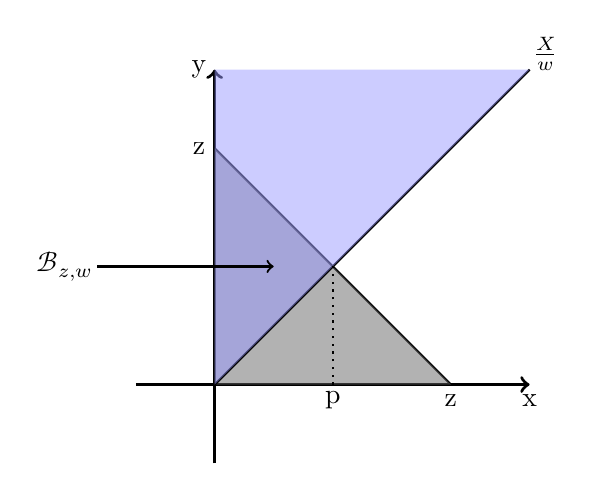
\begin{tikzpicture}
  \draw[very thick, ->] (-1,0) -- (4,0);
  \draw[very thick, ->] (0,-1) -- (0,4);
  \node at (4,-0.2) {x};
  \node at (-0.2,4) {y};
  \node at (3,-0.2) {z};
  \node at (-0.2,3) {z};
  \draw[thick] (0,3) -- (3,0);
  \fill[fill=black!60!white, opacity=0.5] (0, 0) -- (3, 0) -- (0, 3);
  \draw[thick] (0,0) -- (4,4);
  \node at (4.2,4.2) {$\frac{X}{w}$};
  \fill[fill=white!60!blue, opacity=0.5] (0, 0) -- (4, 4) -- (0, 4);
  \node at (-1.9,1.5) {$\mathcal{B}_{z,w}$};
  \draw[thick, <-] (0.75,1.5) -- (-1.5,1.5);
  \node at (1.5,-0.2) {p};
  \draw[thick,dotted] (1.5,0) -- (1.5,1.5);
\end{tikzpicture}
\end{center}

Onde a região em azul claro são os valores onde \(Y \ge \frac{X}{w}\), e a região cinza são os valores em que \(Y \le z - X\), o ponto \(p\) é dado por:

\begin{align*}
\frac{X}{w} = z - X \Rightarrow z &= X \left(\frac{1}{w} +1\right) \\
z &= X\left(\frac{w+1}{w}\right) \\
X &= \frac{zw}{w+1}
\end{align*}

Assim, estamos interessados em encontrar \(P((X,Y) \in \mathcal{B}_{z,w})\), que será:

\begin{align*}
P((X,Y) \in \mathcal{B}_{z,w}) &= \int_{0}^{p}\int_{\frac{x}{w}}^{z-x}e^{-x}e^{-y}dydx \\
&= \int_{0}^{\frac{zw}{w+1}}e^{-x}\left[-e^{-y}\big{|}_{\frac{x}{w}}^{z-x}\right]dx \\
&= \int_{0}^{\frac{zw}{w+1}}e^{-x}\left[e^{-\frac{x}{w}-e^{-z+x}}\right]dx \\
&= \int_{0}^{\frac{zw}{w+1}}e^{-x\left(\frac{1 + w}{w}\right)}-e^{-z}dx \\
&= -\frac{w}{(1+w)}e^{-x\left(\frac{1 + w}{w}\right)}\bigg{|}_{0}^{\frac{zw}{w+1}}-e^{-z}x\bigg{|}_{0}^{\frac{zw}{w+1}} \\
&= \frac{w}{1+w}\left(1-e^{-z}-ze^{-z}\right)
\end{align*}

Assim, temos que a distribuição de \(Z\) e \(W\) será dada por:

\begin{equation*}
F_{ZW}(z,w) = \begin{cases}
0 & ,z \le 0, w \le 0 \\
\frac{w}{1+w}\left(1-e^{-z}-ze^{-z}\right) & ,z > 0, w > 0
\end{cases}
\end{equation*}

Que é uma distribuição de probabilidade, pois é absolutamente contínua (e por consequência, contínua à direita) e os seguintes limites são bem definidos:

\begin{align*}
\lim_{w \to 0}F_{ZW}(z,w) &= 0 \\
\lim_{z \to 0}F_{ZW}(z,w) &= 0 \\
\lim_{z \to \infty, w \to \infty}F_{ZW}(z,w) &= 1
\end{align*}

\textbf{b)}

Temos que as distribuições marginais de \(Z\) e \(W\) serão:

\begin{align*}
F_{Z}(z) &= \lim_{w \to \infty}F_{ZW}(z,w) = 1-e^{-z}-ze^{-z} \\
F_{W}(w) &= \lim_{z \to \infty}F_{ZW}(z,w) = \frac{w}{1+w}
\end{align*}

E como a distribuição conjunta é o produto das marginais, temos que \(Z \perp W\). As densidades serão dadas pelas derivadas da distribuição acumulada conjunta, ou seja:

\begin{align*}
f_{ZW}(z,w) &= \frac{\partial}{\partial z}\frac{\partial}{\partial w}\left(\frac{w}{1+w}\left(1-e^{-z}-ze^{-z}\right)\right) \\
&= \frac{1}{(1+w)^{2}}ze^{-z}I_{(0,\infty)}(z)I_{(0,\infty)}(w)
\end{align*}
\end{example}

\hypertarget{muxe9todo-do-jacobiano}{%
\subsection{Método do Jacobiano}\label{muxe9todo-do-jacobiano}}

Seja \(g:G_{0} \to G\), com \(G,G_{0} \subseteq \mathbb{R}^{n}\) e ambos abertos. Então \(g(x_{1},\ldots,x_{n}) = \left(g_{1}(x_{1},\ldots,x_{n}),\ldots,g_{n}(x_{1},\ldots,x_{n})\right) = (y_{1},\ldots,y_{n})\), com \(g\) sendo bijetiva, ou seja, para todo \(y\) valor de \(Y\), existe \(\underbar{x}\) valor de \(X\) tal que \(g(\underbar{x}) = y\).

Logo \(g\) admite inversa usual \(g^{-1} = h\), com \(h = (h_{1}, \ldots, h_{n})\):

\begin{align*}
&x_{1} = h_{1}(y_{1},\ldots,y_{n}) \\
&\vdots \\
&x_{n} = h_{n}(y_{1},\ldots,y_{n})
\end{align*}

Vamos supor que existem as derivadas parciais \(\frac{\partial x_{i}}{\partial y_{j}}, \forall i, \forall j\), e que elas são contínuas em \(G\). Desejamos computar: \(\int \ldots \int_{C}f_{Y}(y)dy\) ,em termos de \(\int \ldots \int_{D}f_{X}(x)dx\).

\begin{example}
Sejam \(Y = (Y_{1},Y_{2}) = \left(X_{1} + X_{2}, \frac{X_{1}}{X_{2}}\right)\). Teremos então que: \(y_{1} = g_{1}(x_{1},x_{2}) = x_{1} + x_{2}\) e \(y_{2} = g_{2}(x_{1},x_{2}) = \frac{x_{1}}{x_{2}}\). Temos assim os valores dos \(y\)'s em termos dos \(x\)'s, e desejamos encontrar o contrário:

\begin{align*}
y_{1} &= x_{1} + x_{2} \Rightarrow x_{1} = y_{1} - x_{2} \\
y_{2} &= \frac{y_{1}-x_{2}}{x_{2}} \Rightarrow x_{2} = \frac{y_{1}}{y_{2}+1} \Rightarrow x_{1} = \frac{y_{1}y_{2}}{y_{2} + 1}
\end{align*}

Agora que temos os valores de \(X_{1}\) e \(X_{2}\) em função de \(Y_{1}\) e \(Y_{2}\). Agora, podemos calcular as derivadas parciais de \(x\) com relação a \(y\):

\begin{align*}
\frac{\partial x_{1}}{\partial y_{1}} &= y_{2}(y_{2} + 1)^{-1} \\
\frac{\partial x_{1}}{\partial y_{2}} &= y_{1}(y_{2} + 1)^{-2} \\
\frac{\partial x_{2}}{\partial y_{1}} &= (y_{2} + 1)^{-1} \\
\frac{\partial x_{2}}{\partial y_{2}} &= -y_{1}(y_{2} + 1)^{-2}
\end{align*}

Definimos agora o Jacobiano:

\begin{equation}
J(\underbar{x},\underbar{y}) = \det \begin{bmatrix}
\frac{\partial x_{1}}{\partial y_{1}} & \frac{\partial x_{1}}{\partial y_{2}} & \hdots & \frac{\partial x_{1}}{\partial y_{n}} \\
\frac{\partial x_{2}}{\partial y_{1}} & \frac{\partial x_{2}}{\partial y_{2}} & \hdots & \frac{\partial x_{2}}{\partial y_{n}} \\
\vdots & \vdots  & \ddots & \vdots \\
\frac{\partial x_{n}}{\partial y_{1}} & \frac{\partial x_{n}}{\partial y_{2}} & \hdots & \frac{\partial x_{n}}{\partial y_{n}}
\end{bmatrix}
\label{eq:jacobiano}
\end{equation}

Dessa forma, o Jacobiano da transformação será:

\begin{align*}
J(\underbar{x},\underbar{y}) &= \det \begin{bmatrix}
y_{2}(y_{2} + 1)^{-1} & y_{1}(y_{2} + 1)^{-2} \\
(y_{2} + 1)^{-1} & -y_{1}(y_{2} + 1)^{-2}
\end{bmatrix} \\
&= [y_{2}(y_{2} +1)^{-1}].[-y_{1}(y_{2}+1)^{-2}] - [y_{1}(y_{2} + 1)^{-2}].[(y_{2} + 1)^{-1}] \\
&= -y_{1}(y_{2} + 1)^{-2}
\end{align*}

Pelo teorema do Jacobiano, temos que:

\begin{equation*}
\int \ldots \int_{A}f(x_{1}, \ldots, x_{n})dx_{1} \ldots dx_{n} = \int \ldots \int_{g(A)}f(h_{1}(y_{1}, \ldots, y_{n}), \ldots , h_{n}(y_{1}, \ldots, y_{n}))|J(\underbar{x}, \underbar{y})|dy_{1} \ldots dy_{n}
\end{equation*}

Se \(f\) é integrável em \(A\), com \(A \subseteq G_{0}\) e \(h = g^{-1}\). Assim, usando os valores do exemplo \ref{exm:motivacaoexponencial}, temos que \(X_{1} \sim exp(1), X_{2} \sim exp(1), X_{1} \perp X_{2}\), com densidade conjunta dada por \$ f\_\{X\_\{1\}X\_\{2\}\}(x\_\{1\},x\_\{2\}) = e\^{}\{-x\_\{1\} + x\_\{2\}\}\$, de modo que:

\begin{align*}
f(h_{1}(y_{1},y_{2}),h_{2}(y_{1},y_{2}))|J(\underbar{x},\underbar{y})| &= f\left(\frac{y_{1}y_{2}}{y_{2} + 1},\frac{y_{1}}{y_{2} + 1}\right)\big{|}-y_{1}(y_{2} + 1)^{-2}\big{|} \\
&= \exp\left(-\left[\frac{y_{1}y_{2}}{y_{2} + 1}+\frac{y_{1}}{y_{2} + 1}\right]\right)y_{1}(y_{2} + 1)^{-2} \\
&= e^{-y_{1}}y_{1}(y_{2} + 1)^{-2}
\end{align*}

Que é a mesma densidade conjunta encontrada para \(Z\) e \(W\) no exemplo \ref{exm:motivacaoexponencial}.
\end{example}

\hypertarget{notas}{%
\subsubsection{Notas}\label{notas}}

\begin{enumerate}
\def\labelenumi{\arabic{enumi}.}
\tightlist
\item
  Sendo \(f\) a densidade de \(X_{1}, \ldots, X_{n}\) e \(P((X_{1}, \ldots, X_{n}) \in G_{0}) = 1\), se \(Y_{i} = g_{i}(x_{1}, \ldots, x_{n}); i = 1, \ldots, n\), e \(\mathcal{B} \subseteq G\), com \(\mathcal{B}\) boreliano. Então:
\end{enumerate}

\begin{align*}
P((Y_{1},\ldots,Y_{n}) \in \mathcal{B}) &= P((X_{1}, \ldots, X_{n}) \in h(\mathcal{B})) \\
&= \int \dots \int_{h(\mathcal{B})}f(x_{1},\ldots,x_{n})dx_{1} \ldots dx_{n} \\
&= \int \dots \int_{\mathcal{B}}f(h_{1}(x_{1}, \ldots, x_{n}),\ldots,h_{n}(x_{1},\ldots,x_{n}))\big{|}J(\underbar{x},\underbar{y})\big{|}dy_{1} \ldots dy_{n}
\end{align*}

\begin{enumerate}
\def\labelenumi{\arabic{enumi}.}
\setcounter{enumi}{1}
\tightlist
\item
  \(P((Y_{1},\ldots,Y_{n}) \in G) = P((X_{1}, \ldots, X_{n}) \in h(G)) = P((X_{1}, \ldots, X_{n}) \in G_{0}) = 1\). De modo análogo:
\end{enumerate}

\begin{align*}
P((Y_{1}, \ldots, Y_{n}) \in \mathcal{B}) &= P((Y_{1}, \ldots, Y_{n}) \in \mathcal{B} \cap G) \\
&= \int \dots \int_{\mathcal{B} \cap G}f(h(y))\big{|}J(\underbar{x},\underbar{y})\big{|}dy_{1} \ldots dy_{n}
\end{align*}

\begin{theorem}
Sob as condições impostas no início da seção, a densidade conjunta de \((Y_{1}, \ldots, Y_{n})\) é dada por:

\begin{equation*}
f_{Y_{1}\ldots Y_{n}} = \begin{cases}
f_{X}(h_{1}(y_{1},\ldots,y_{n}), \ldots, h_{n}(y_{1},\ldots,y_{n}))\big{|}J(\underbar{x},\underbar{y})\big{|} & ,y \in G \\
0 & ,c.c.
\end{cases}
\end{equation*}
\end{theorem}

\hypertarget{propriedades-do-jacobiano}{%
\subsubsection{Propriedades do Jacobiano}\label{propriedades-do-jacobiano}}

Podemos inverter a ordem das variáveis no Jacobiano, seguindo a seguinte propriedade:

\begin{equation}
J(\underbar{x},\underbar{y}) = \left(J(\underbar{y},\underbar{x})\right)^{-1}\big{|}_{\underbar{x} = h(y)}
\label{eq:inversajacobiano}
\end{equation}

\begin{example}
Retornando ao problema apresentado no exemplo \ref{exm:motivacaoexponencial}:

\begin{align*}
y_{1} = x_{1} + x_{2} \; \; &\; \; \; y_{2} = x_{1}x_{2}^{-1} \\
\frac{\partial y_{1}}{\partial x_{1}} = 1 \; \; &\; \; \; \frac{\partial y_{1}}{\partial x_{2}} = 1 \\
\frac{\partial y_{2}}{\partial x_{1}} = x_{2}^{-1} \; \; &\; \; \; \frac{\partial y_{2}}{\partial x_{2}} = -x_{1}(x_{2})^{-2}
\end{align*}

De modo que podemos agora encontrar o Jacobiano com relação aos valores das derivadas parciais dos \(y\)'s, e invertê-lo para encontrar o Jacobiano dos \(x\)'s:

\begin{align*}
J(\underbar{y},\underbar{x}) = \det \begin{bmatrix}
1 & 1 \\
x_{2}^{-1} & -x_{1}(x_{2})^{-2}
\end{bmatrix} &= (x_{2})^{-2}(x_{2} + x_{1})(-1) \\
&= \left(\frac{y_{2} + 1}{y_{1}}\right)^{2}\left(\frac{y_{1}}{y_{2} + 1} + \frac{y_{1}y_{2}}{y_{2} + 1}\right)(-1) \\
&= \frac{(y_{2} + 1)^{2}}{(y_{1})^{2}}\frac{y_{1}(y_{2} + 1)}{y_{2} + 1}(-1) \\
&= -\frac{(y_{2} + 1)^{2}}{y_{1}} = -y_{1}^{-1}(y_{2} + 1)^{2} = \frac{1}{J(\underbar{x},\underbar{y})}
\end{align*}
\end{example}

Temos que, se \(g:G_{0} \to G\), com \(G_{0},G \subseteq \mathbb{R}^{n}\) abertos, se \(g(x_{1}, \ldots, x_{n}) = (y_{1}, \ldots, y_{n})\), então \(g\) é bijetiva e \(h = g^{-1}\).

\begin{example}
Seja \(X \sim U(0,1)\) e \(Y = -ln(X)\). Temos que \(G_{0} = (0,1)\), e \(g(x) = -ln(x)\), de modo que \(G = (0, \infty)\). Então:

\begin{align*}
g^{-1}(y) &= h(y) = \exp(-y) = e^{-y} \\
\frac{\partial}{\partial y}(g^{-1}(y)) &= -e^{-y} = J(x,y)
\end{align*}

Assim, para encontrar \(P(Y \le y)\), teremos:

\begin{align*}
P(Y \le y) &= P(-\ln(X) \le y) \\
&= P(\ln(X) \ge -y) \\
&= P(X \ge e^{-y}) \\
&= 1 - P(X \le e^{-y}) \\
&= 1 - e^{-y} = F_{Y}(y) \Longrightarrow f_{Y}(y) = e^{-y}
\end{align*}

Pelo Jacobiano, teremos:

\begin{equation*}
f_{Y}(y) = f_{X}(h(y)).|J| = 1 . e^{-y}
\end{equation*}
\end{example}

\begin{theorem}
Sejam \(G_{1}, G_{2}, \ldots, G_{k}\) disjuntos tais que \(P\left(\underbar{X} \in \bigcup_{i=1}^{k}G_{i}\right) = 1\), tal que \(g\big{|}_{G_{l}}\) é 1:1 para todo \(l = 1, \ldots, k\). Denotamos por \(h^{(l)}\) a inversa de \(g\) em \(G_{l}\), e definimos assim o Jacobiano local \(J_{l}(\underbar{x},\underbar{y})\) como:

\begin{equation*}
f_{Y}(\underbar{y}) = \begin{cases}
\sum_{l=1}^{k}f\left(h^{(l)}(y)\right)|J_{l}(\underbar{x},\underbar{y})| & ;\underbar{y} \in G_{l} \\
0 & c.c.
\end{cases}
\end{equation*}
\end{theorem}

\begin{example}
Sejam \(X \sim N(0,1)\) e \(Y = X^{2}\). Sabemos que \(y = x^{2}\) não é bijetiva, mas podemos considerar a seguinte partição em que essa função seja localmente bijetiva: \(G_{1} = (-\infty, 0)\) e \(G_{2} = (0, \infty)\). Então, em \(G_{1}, h^{(1)}(y) = -\sqrt{y}\), e em \(G_{2}, h^{(2)}(y) = \sqrt{y}\), de modo que os jacobianos locais serão:

\begin{align*}
J_{1}(x,y) &= \frac{\partial}{\partial y}h^{(1)}(y) = - \frac{1}{2\sqrt{y}} \\
J_{2}(x,y) &= \frac{\partial}{\partial y}h^{(2)}(y) = \frac{1}{2\sqrt{y}}
\end{align*}

Assim, a densidade de \(Y\) será dada por:

\begin{align*}
f_{Y}(y) &= f_{X}\left(h^{(1)}(y)\right)\big{|}J_{1}(x,y)\big{|} + f_{X}\left(h^{(2)}(y)\right)\big{|}J_{2}(x,y)\big{|} \\
&= \frac{1}{\sqrt{2\pi}}\exp\left(-\frac{1}{2}y\right)\frac{1}{2\sqrt{y}} + \frac{1}{\sqrt{2\pi}}\exp\left(-\frac{1}{2}y\right)\frac{1}{2\sqrt{y}} \\
&= \begin{cases}
\frac{1}{\sqrt{2\pi}}y^{-\frac{1}{2}}e^{-\frac{1}{2}y} & ,y>0 \\
0 & ,c.c.
\end{cases}
\end{align*}

Ou seja, \(Y \sim Gama\left(\frac{1}{2}, \frac{1}{2}\right)\), ou \(Y \sim \chi^{2}(1)\).
\end{example}

\textbf{Notas}:

\begin{itemize}
\tightlist
\item
  Se \(X_{1}, \ldots, X_{n}\) são iid, com \(X_{i} \sim N(0,1) \Rightarrow X_{1}^{2} + \ldots + X_{n}^{2} \sim \chi^{2}(n)\);
\item
  Se \(X \sim N(0,1), Y \sim \chi^{2}(n)\), com \(X \perp Y \Rightarrow \frac{x}{\sqrt{y/n}} \sim t(n)\);
\item
  Sejam \(X_{1}, \ldots, X_{n}\), iid, com \(X_{i} \sim N(0,1)\), com \(\bar{x} = \frac{\sum_{i=1}^{n}x_{i}}{n}, s^{2} = \frac{1}{n-1}\sum_{i=1}^{n}(x_{i} - \bar{x})^{2}\):

  \begin{enumerate}
  \def\labelenumi{\arabic{enumi}.}
  \tightlist
  \item
    \(\frac{\bar{x}\sqrt{n}}{\sigma} \sim N(0,1)\);
  \item
    \(\frac{(n-1)s^{2}}{\sigma^{2}} \sim \chi^{2}(n-1)\);
  \item
    \(\frac{\bar{x}\sqrt{n}}{s} \sim t(n-1)\);
  \item
    \(\bar{x} \perp s^{2}\).
  \end{enumerate}
\item
  Se \(X \sim \chi^{2}(k), Y \sim \chi^{2}(n), X \perp Y \Rightarrow \frac{X/k}{Y/n} \sim F(k,n)\);
\item
  Se \(T \sim t(n) \Rightarrow T^{2} \sim F(1,n)\).
\end{itemize}

\newpage

\hypertarget{exercuxedcios-1}{%
\subsection{Exercícios}\label{exercuxedcios-1}}

TODO

\newpage

\hypertarget{esperanuxe7a}{%
\section{Esperança}\label{esperanuxe7a}}

\hypertarget{definiuxe7uxe3o}{%
\subsection{Definição}\label{definiuxe7uxe3o}}

\begin{definition}
Se \(X\) é uma variável aleatória com distribuição \(F\), a esperança de \(X\) é definida por \(E(X = \int_{-\infty}^{\infty}x dF(x)\), sempre que a integral estiver bem definida.
\end{definition}

\textbf{Convenção}: Se \(E(X) < \infty\), então \(X\) é integrável.

\textbf{Nota}: \(\int_{-\infty}^{\infty}xdF(x)\) é bem definida se \(\int_{0}^{\infty}xdF(x)\) ou \(\int_{-\infty}^{0}xdF(x)\) for finita, já que \(\int_{-\infty}^{\infty}xdF(x) = \underbrace{\int_{-\infty}^{0}xdF(x)}_{\mathclap{\mathbf{I} \le 0}} + \underbrace{\int_{0}^{\infty}xdF(x)}_{\mathclap{\mathbf{II} \ge 0}}\). Assim, podemos separar em quatro casos:

\begin{enumerate}
\def\labelenumi{\arabic{enumi}.}
\tightlist
\item
  Se \textbf{I} e \textbf{II} são finitos, então \(X\) é integrável;
\item
  Se \textbf{I} é finito e \(\mathbf{II} = +\infty\), então \(E(X) = +\infty\);
\item
  Se \textbf{II} é finito e \(\mathbf{I} = -\infty\), então \(E(X) = -\infty\);
\item
  Se \(\mathbf{I} = -\infty\) e \(\mathbf{II} = +\infty\), então \(E(X)\) é indefinida.
\end{enumerate}

\textbf{Propriedade}: \(E(|X|) = \int |x| dF(x)\). Logo, \(X\) é integrável se e somente se \(E(|X|) < \infty\).

\begin{example}
\(X \sim U(0,1),\; Y = \min\left(X,\frac{1}{2}\right)\):

\begin{align*}
P\left(Y = \frac{1}{2}\right) &= P\left(X > \frac{1}{2}\right) = 1 - F_{X}\left(\frac{1}{2}\right) = 1 - \frac{1}{2} = \frac{1}{2} = P_{Y}\left(Y = \frac{1}{2}\right)\\
E(Y) = \int_{-\infty}^{\infty}ydF(y) &= \int_{0}^{1/2}y.1dy + \frac{1}{2}P_{Y}\left(Y=\frac{1}{2}\right) \\
&= \frac{y^{2}}{2}\bigg{|}_{0}^{1/2} + \frac{1}{4} \\
&= \frac{1}{8} + \frac{1}{2} = \frac{3}{8}
\end{align*}
\end{example}

\begin{proposition}
\protect\hypertarget{prp:separespe}{}\label{prp:separespe}

\(E(X) = \int_{0}^{\infty}(1 - F(x))dx - \int_{-\infty}^{0}F(x)dx\). Disso, temos que:

\begin{itemize}
\tightlist
\item
  \textbf{a)} \(\int_{0}^{\infty}xdF(x) = \int_{0}^{\infty}(1 - F(x))dx\);
\item
  \textbf{b)} \(\int_{-\infty}^{0}xdF(x) = - \int_{-\infty}^{0}F(x)dx\);
\end{itemize}

\end{proposition}

\begin{proof}[Prova]
Vejamos \textbf{(a)}: considere que \(d(xF(x)) = F(x)dx + xd(F(x)) \Rightarrow xd(F(x)) = d(xF(x)) - F(x)dx\). Seja um \(b > 0\):

\begin{align*}
\int_{0}^{b}xdF(x) &= \int_{0}^{b}d(xF(x)) - \int_{0}^{b}F(x)dx \\
&= xF(x)\bigg{|}_{0}^{b} - \int_{0}^{b}F(x)dx \\
&= bF(b) - \int_{0}^{b}F(x)dx \\
&= \int_{0}^{b}[F(b) - F(x)]dx
\end{align*}

Note que \(\int_{0}^{b}xdF(x) \le \int_{0}^{\infty}[1 - F(x)]dx, \; \forall b>0\). Basta notar que \(F(b) - F(x) \le 1 - F(x)\) e que \(\int_{0}^{b}[1 - F(x)]dx \le \int_{0}^{\infty}[1 - F(x)]dx\). Logo:

\begin{equation*}
\int_{0}^{\infty}xdF(x) = \lim_{b \to \infty}\int_{0}^{b}xdF(x) \le \int_{0}^{\infty}[1 - F(x)]dx \Rightarrow \int_{0}^{\infty}xdF(x) \le \int_{0}^{\infty}[1 - F(x)]dx
\end{equation*}

Considere \(\lambda > 0\) e \(b > 0\), tais que:

\begin{align*}
\int_{0}^{b}[F(b) - F(x)]dx \ge \int_{0}^{\lambda}[1 - F(x)]dx &= \int_{0}^{\lambda}[F(b) - 1]dx + \int_{0}^{\lambda}[1 - F(x)]dx \\
&= \lambda[F(b) - 1] + \int_{0}^{\lambda}[1 - F(x)]dx \\
\int_{0}^{b}[F(b) - F(x)]dx &\ge \lambda[F(b) - 1] + \int_{0}^{\lambda}[1 - F(x)]dx
\end{align*}

Logo, como \(\int_{0}^{\infty}xdF(x) = \lim_{b \to \infty}\int_{0}^{b}[F(b) - F(x)]dx \ge \lim_{b \to \infty}\{\lambda[F(b) - 1] + \int_{0}^{\lambda}[1 - F(x)]dx\} = \int_{0}^{\lambda}[1 - F(x)]dx\). Assim:

\begin{equation*}
\int_{0}^{\infty}xdF(x) \ge \lim_{\lambda \to \infty}\int_{0}^{\lambda}[1 - F(x)]dx = \int_{0}^{\infty}[1 - F(x)]dx
\end{equation*}

E como \(\int_{0}^{\infty}xdF(x) \le \int_{0}^{\infty}[1 - F(x)]dx\), temos que \(\int_{0}^{\infty}xdF(x) = \int_{0}^{\infty}[1 - F(x)]dx\)
\end{proof}

\begin{corollary}
\protect\hypertarget{cor:esppositiva}{}\label{cor:esppositiva}Se \(X\) é tal que \(X(\omega) \ge 0 \; \forall \omega \in \mathbb{R} \Rightarrow E(X) = \int_{0}^{\infty}[1 - F(x)]dx = \int_{0}^{\infty}P(X \ge x)dx\).
\end{corollary}

\begin{example}
Seja \(X \sim Exp(\lambda)\), qual a \(E(X)\)? Como o suporte de \(X\) é \((0,\infty)\), aplica-se o corolário anterior, de modo que:

\begin{align*}
F_{X}(x) &= 1 - e^{-\lambda x} \Leftrightarrow P(X > x) = e^{-\lambda x} \\
E(X) &= \int_{0}^{\infty}e^{-\lambda x}dx = -\frac{1}{\lambda}e^{-\lambda x}\bigg{|}_{0}^{\infty} = \frac{1}{\lambda}
\end{align*}
\end{example}

\textbf{Nota}: Suponha \(X\) discreta e \(X(\omega) \ge 0 \; \forall \omega\). Então:

\begin{align*}
E(X) = \sum_{n=0}^{\infty}P(X > n) &= \sum_{n=0}^{\infty}P(X \ge n+1) \\
&= \sum_{n=1}^{\infty}P(X \ge n)
\end{align*}

\begin{example}
Considere o lançamento de uma moeda até a 1ª cara. Suponha \(p=\) probabilidade de cara e \((1 - p) =\) probabilidade de coroa, e \(X =\) número de lançamentos até a primeira cara. Tome o evento \([X \ge n]\), logo:

\begin{equation*}
E(X) = \sum_{n=1}^{\infty}(1 - p)^{n-1} = \sum_{n=0}^{\infty}(1 - p)^{n} = \frac{1}{p}
\end{equation*}
\end{example}

\textbf{Nota}: Sendo \(X\) uma variável aleatória, temos pelo corolário \ref{cor:esppositiva} que:

\begin{align*}
E(|X|) &= \int_{0}^{\infty}P(|X| > x)dx \\
&= \int_{0}^{\infty}\big[P(X > x) + P(X < -x)\big]dx \\
&= \int_{0}^{\infty}P(X > x)dx + \int_{0}^{\infty}P(X < -x)dx \\
&= \int_{0}^{\infty}(1-F(x))dx + \int_{0}^{\infty}F((-x)^{-})dx
\end{align*}

Onde \(F((-x)^{-}) = \lim_{u \uparrow -x}F(u)\), que caso \(F\) seja contínua, coincide com \(F(-x)\). Logo:

\begin{equation*}
E(|X|) = \int_{0}^{\infty}(1 - F(x))dx + \int_{0}^{\infty}F(-x)dx
\end{equation*}

Já que \(F\) pode ser descontínua em uma coleção enumerável de pontos. Agora, tomando a transformação de variável \(y = -x \Leftrightarrow dy = -dx\):

\begin{align*}
E(|X|) &= \int_{0}^{\infty}(1 - F(x))dx + \int_{-\infty}^{0}F(y)dy \\
&= \int_{0}^{\infty}(1 - F(x))dx + \int_{-\infty}^{0}F(x)dx
\end{align*}

Utilizando os resultados \textbf{a} e \textbf{b} da proposição \ref{prp:separespe}, temos que:

\begin{align*}
E(|X|) &= \int_{0}^{\infty}xdF(x) - \int_{-\infty}^{0}xdF(x) \\
&= \int_{0}^{\infty}|x|dF(x) + \int_{-\infty}^{0}|x|dF(x) \\
&= \int_{-\infty}^{\infty}|x|dF(x)
\end{align*}

Onde \(F\) é a acumulada de \(X\), ao invés de \(|X|\). Assim, a integrabilidade de \(X\) depende da finitude de \(\int_{0}^{\infty}xdF(x)\) e \(\int_{-\infty}^{0}xdF(x)\), logo \(X\) é integrável se \(E(|X|) < \infty\).

\hypertarget{propriedades-da-esperanuxe7a}{%
\subsection{Propriedades da esperança}\label{propriedades-da-esperanuxe7a}}

\begin{itemize}
\tightlist
\item
  \(\mathbf{E_{1}}\): Se \(X = c\), com \(c\) uma constante, \(E(X) = c\);
\item
  \(\mathbf{E_{2}}\)\textbf{(monotonia)}: Se \(X\) e \(Y\) são variáveis aleatórias, com \(X \le Y \Rightarrow E(X) \le E(Y)\), caso ambas as esperanças estejam bem definidas;
\end{itemize}

\begin{proof}[Prova]
Seja \(z\) um valor fixo. Se \(Y \le z \Rightarrow X \le z\), logo \([Y \le z] \subseteq [X \le z]\), assim:

\begin{align*}
P(Y \le z) &\le P(X \le z) \\
F_{Y}(z) &\le F_{X}(z) \Longleftrightarrow 1 - F_{Y}(z) \ge 1 - F_{X}(z)
\end{align*}

E pela proposição \ref{prp:separespe}, temos que:

\begin{align*}
E(Y) = \int_{0}^{\infty}\big{[}1 - F_{Y}(z)\big{]}dz - \int_{-\infty}^{0}F_{Y}(z)dz &\ge \int_{0}^{\infty}\big{[}1 - F_{X}(z)\big{]}dz - \int_{-\infty}^{0}F_{X}(z)dz = E(X) \\
E(Y) &\ge E(X)
\end{align*}
\end{proof}

\begin{itemize}
\tightlist
\item
  \(\mathbf{E_{3}}\)\textbf{(linearidade)}:

  \begin{itemize}
  \tightlist
  \item
    \textbf{(i)} Se \(E(X)\) é bem definida, \(a,b \in \mathbb{R}\), então \(E(aX + b) = aE(X) + b\);
  \item
    \textbf{(ii)} \(E(aX + bY) = aE(X) + bE(Y)\), caso o termo \(aE(X) + bE(Y)\) esteja bem definido;
  \item
    Note que se \(E(X) = \infty \Rightarrow E(X - X) \neq E(X) - E(X)\).
  \end{itemize}
\end{itemize}

\begin{proof}[Prova]
Quando \(a = 0; E(aX + b) = E(b) = b = 0E(X) + b\).

Quando \(a > 0, b > 0; F_{aX + b}(x) = P(aX+b \le x) = P\left(X \le \frac{x-b}{a}\right) = F_{X}\left(\frac{x-b}{a}\right)\). Logo:

\begin{align*}
E(aX + b) &= \int_{0}^{\infty}\big{[}1 - F_{aX + b}(x)\big{]}dx - \int_{-\infty}^{0}F_{aX + b}(x)dx \\
&= \int_{0}^{\infty}\left[1 - F_{X}\left(\frac{x-b}{a}\right)\right]dx - \int_{-\infty}^{0}F_{X}\left(\frac{x-b}{a}\right)dx
\end{align*}

Tome \(y = \frac{x-b}{a} \Rightarrow dy = \frac{1}{a}dx\). Então:

\begin{align*}
E(aX+b) &= \int_{-b/a}^{\infty}a\big{[}1 - F_{X}(y)\big{]}dy - \int_{-\infty}^{-b/a}aF_{X}(y)dy \\
&= a\left\{\int_{-b/a}^{\infty}\big{[}1 - F_{X}(y)\big{]}dy - \int_{-\infty}^{-b/a}F_{X}(y)dy\right\} \\
&= a\int_{0}^{\infty}\big{[}1 - F_{X}(y)\big{]}dy - a\int_{-\infty}^{0}F_{X}(y)dy + a\int_{-b/a}^{0}\big{[}1 - F_{X}(y)\big{]}dy + a\int_{-b/a}^{0}F_{X}(y)dy \\
&= aE(X) + a \int_{-b/a}^{0}dy \\
&= aE(X) + a \frac{b}{a} \\
&= aE(X) + b
\end{align*}
\end{proof}

\begin{itemize}
\tightlist
\item
  \(\mathbf{E_{4}}\)\textbf{(Desigualdade de Jansen)}: Seja \(\varphi\) uma função convexa, definida na reta, com \(X\) integrável, então:
\end{itemize}

\begin{equation}
E(\varphi(X)) \ge \varphi(E(X))
\label{eq:desigjansen}
\end{equation}

\textbf{Nota}: Caso \(\varphi\) seja côncava:

\begin{equation*}
E(\varphi(X)) \le \varphi(E(X))
\end{equation*}

\begin{proof}[Prova para convexa]
Tome \(x_{0}\) e \(\varphi(x_{0})\). Então existe uma reta \(L\) tal que \(L\) passe por \(\varphi(x_{0})\) e \(\varphi\) fica por cima de \(L\). Logo temos a seguinte equação da reta:

\begin{equation*}
L(x) = \varphi(x_{0}) + \lambda(x - x_{0})
\end{equation*}

Onde \(\lambda\) é alguma constante apropriada. Então para todo \(x\) temos:

\begin{align*}
\varphi(x) &\ge L(x) = \varphi(x_{0}) + \lambda(x - x_{0}) \\
&\big{\Downarrow} \;\mathbf{E_{2}} \\
E(\varphi(x)) &\ge E(L(x)) \stackrel{\mathbf{E_{1},E_{3}}}{=} \varphi(x_{0}) + \lambda\left[E(x) - x_{0}\right]
\end{align*}

Que vale para \(x_{0} = E(x)\), de modo que \(E(\varphi(x)) \ge \varphi(E(x)) + \lambda\left[E(x) - E(x)\right]\), então:

\begin{equation*}
E(\varphi(x)) \ge \varphi(E(x))
\end{equation*}

A prova para funções côncavas segue a mesma metodologia, com a inversão da desigualdade.
\end{proof}

\hypertarget{crituxe9rio-de-integrabilidade}{%
\subsubsection{Critério de integrabilidade}\label{crituxe9rio-de-integrabilidade}}

Suponha que \(X\) é uma variável aleatória dominada por \(Y\) (ou seja, \(X \le Y\)), sendo \(Y\) uma variável aleatória integrável. \(X\) é integrável? Temos que:

\begin{equation*}
X \le Y \Rightarrow E(X) \le E(Y)
\end{equation*}

Se \(X\) e \(Y\) são tais que \(Y \ge 0\) e \(Y\) é integrável e \(|X| \le Y \Rightarrow 0 \le |X| \le Y\), e como consequência:

\begin{equation*}
0 \le E(X) \le E(Y) < \infty \Longrightarrow X \text{ é integrável}
\end{equation*}

De maneira similar, seja \(X\) uma variável aleatória qualquer. Então:

\begin{equation*}
\sum_{n=1}^{\infty}P(|X| \ge n) \le E(|X|) \le 1 + \sum_{n=1}^{\infty}P(|X| \ge n)
\end{equation*}

Assim, \(X\) é integrável se e somente se \(\sum_{n=1}^{\infty}P(|X| \ge n) < \infty\).

\begin{proof}[Prova]
Seja \(x \ge 0\). Tome \([x]\) como a parte inteira de \(x\). Então \([|x|] = k\) se \(k \le |x| < k+1\). Então:

\begin{align*}
0 \le [|x|] &\le |x| \le [|x|] + 1 \\
&\Downarrow \; \mathbf{E_{2},E_{3}} \\
0 \le E([|x|]) &\le E(|x|) \le E([|x|]) + 1
\end{align*}

Pelo corolário \ref{cor:esppositiva}, como \([|x|]\) é discreta e não-negativa, temos que:

\begin{align*}
E([|x|]) &= \sum_{n=1}^{\infty}P([|x|] \ge n) \\
&= \sum_{n=1}^{\infty}P(|x| \ge n) \le E(|x|) \le \sum_{n=1}^{\infty}P(|x| \ge n) + 1
\end{align*}
\end{proof}

\hypertarget{casos-de-interesse}{%
\subsubsection{Casos de interesse}\label{casos-de-interesse}}

\textbf{a) (Consistência absoluta)} \(\varphi(X) = |X|\):

\begin{equation*}
E(|X|) \ge |E(X)|
\end{equation*}

\textbf{b) (Consistência quadrática)} \(\varphi(X) = X^{2}\):

\begin{equation*}
E(X^{2}) \ge [E(X)]^{2}
\end{equation*}

\textbf{c) (Consistência absoluta de ordem p)} \(\varphi(X) = |X|^{p}, p \ge 1\):

\begin{equation*}
E(|X|^{p}) \ge |E(X)|^{p}
\end{equation*}

\textbf{Nota}: \(\varphi\) só precisa ser convexa (ou côncava) em uma região de probabilidade 1. Por exemplo, se \(X\) é uma variável aleatória, tal que \(P(X > 0) = 1\), ou o suporte da distribuição de \(X\) é \((0, \infty), \varphi(X) = \frac{1}{X}\) é convexa em \((0,\infty) \Rightarrow E\left(\frac{1}{X}\right) \ge \frac{1}{E(X)}\). De modo análogo, se \(P(X > 0) = 1\) e \(\varphi(X) = \ln(X), \varphi\) é côncava em \((0,\infty)\) logo \(E(\ln(X)) \le \ln(E(X))\).

\hypertarget{esperanuxe7a-de-funuxe7uxf5es-de-variuxe1veis-aleatuxf3rias}{%
\subsection{Esperança de funções de variáveis aleatórias}\label{esperanuxe7a-de-funuxe7uxf5es-de-variuxe1veis-aleatuxf3rias}}

Seja \(X\) uma variável aleatória, \(\varphi\) uma função mensurável e \(Y = \varphi(X)\). Assim, \(Y\) é uma variável aleatória, cuja esperança é \(E(Y) = \int ydF_{\varphi(X)}(y) = \int_{0}^{\infty}[1 - F_{\varphi(X)}(y)]dy - \int_{-\infty}^{0}F_{\varphi(X)}(y)dy\).

\begin{theorem}
Se \(X\) é uma variável aleatória e \(\varphi\) uma função mensurável, com \(Y = \varphi(X)\):

\begin{equation*}
E(Y) = E(\varphi(X)) = \int\varphi(x)dF_{X}(x)
\end{equation*}
\end{theorem}

\begin{proof}[Prova para caso $\varphi(x) = x^{k}$]
Note que a prova já foi feita para \(\varphi(x) = |x|\). Vejamos que a prova é válida para \(\varphi(x) = x^{k}\), com \(k = 1,2,\ldots\), em 2 casos: \(k\) par e \(k\) ímpar:

\textbf{\(\mathbf{k}\) par:}

\begin{align*}
E(X^{k}) &= \int_{0}^{\infty}P\left(X^{k} > t\right)dt \\
&= \int_{0}^{\infty}P\left(X > \sqrt[k]{t}\right)dt + \int_{0}^{\infty}P\left(X < - \sqrt[k]{t}\right)dt \\
&= \int_{0}^{\infty}\left[1 - F_{X}\left(\sqrt[k]{t}\right)\right]dt + \int_{0}^{\infty}F_{X}\left(-\sqrt[k]{t}^{\;-}\right)dt
\end{align*}

Apliquemos as seguintes mudanças de variáveis: \(s = t^{\frac{1}{k}}, ds = \frac{1}{k}t^{\frac{1}{k} - 1}dt, dt = \frac{(ds)ks^{k}}{s}, u = -s, du = -ds\):

\begin{align*}
E(X^{k}) &= \int_{0}^{\infty}\left[1-F_{X}(s)\right]ks^{k-1}ds + \int_{0}^{\infty}F_{X}(-s)ks^{k-1}ds \\
&= \int_{0}^{\infty}\left[1-F_{X}(s)\right]ks^{k-1}ds - \int_{-\infty}^{0}F_{X}(u)ku^{k-1}du \\
&= k\left\{\int_{0}^{\infty}[1 - F_{X}(s)]s^{k-1}ds - \int_{-\infty}^{0}F_{X}(u)u^{k-1}du\right\}
\end{align*}

Agora, mostremos que \(E(X^{k}) = \int x^{k}dF_{X}(x)\):

\begin{align*}
\int_{-\infty}^{\infty}x^{k}dF_{X}(x) &\stackrel{Def}{=} \int_{0}^{\infty}\left[1 - F_{X}(x)\right]d(x^{k}) - \int_{-\infty}^{0}F_{X}(x)d(x^{k}) \\
&= k\left\{\int_{0}^{\infty}[1 - F_{X}(x)]x^{k-1}dx - \int_{-\infty}^{0}F_{X}(x)x^{k-1}dx\right\} \\
&= E(X^{k})
\end{align*}
\end{proof}

\textbf{Nota}: A propriedade é também válida para polinômios, visto que a esperança opera de maneira linear.

\begin{example}
Seja \(X \sim Exp(\lambda)\), vimos que \(E(X) = \frac{1}{\lambda}\):

Calcular \(E(X^{2})\):

\begin{align*}
E(X^{2}) = 2\int_{0}^{\infty}xe^{-\lambda x}dx &= \frac{2}{\lambda}\int_{0}^{\infty}x\lambda e^{-\lambda x}dx \\
&= \frac{2}{\lambda}E(X) = \frac{2}{\lambda^{2}}
\end{align*}

Calcular \(E(X^{3})\):

\begin{align*}
E(X^{3}) = 3\int_{0}^{\infty}x^{2}e^{-\lambda x}dx &= \frac{3}{\lambda}\int_{0}^{\infty}x^{2}\lambda e^{-\lambda x}dx \\
&= \frac{3}{\lambda}E(X^{2}) = \frac{3}{\lambda^{3}}
\end{align*}

De modo que podemos observar o padrão emergente, e definir \(E(X^{k}) = \frac{k!}{\lambda^{k}}\).
\end{example}

\hypertarget{momentos-de-uma-variuxe1vel-aleatuxf3ria}{%
\subsection{Momentos de uma variável aleatória}\label{momentos-de-uma-variuxe1vel-aleatuxf3ria}}

\textbf{a)} \(E\left(\left[X - b\right]^{k}\right)\): \(k-\)ésimo momento de \(X\) em torno de \(b\);

\textbf{b)} \(E\left(X^{k}\right)\): \(k-\)ésimo momento em torno de 0;

\textbf{c)} Se em \textbf{(a)}, \(b = E(X)\), o momento é central;

\textbf{d)} \(t>0,E\left(|X|^{t}\right)\): \(t-\)ésimo momento absoluto de \(X\).

\begin{definition}[Variância de uma variável aleatória]
\protect\hypertarget{def:Variancia}{}\label{def:Variancia}\begin{equation*}
\mathrm{Var}(X) = E\left\{(X - E(X))^{2}\right\} \Longleftrightarrow \mathrm{Var}(X) = E\left(X^{2}\right) - \big{(}E(X)\big{)}^{2}
\end{equation*}
\end{definition}

\begin{proposition}
Se \(X\) é uma variável aleatória, \(f(t) = \left[E(|X|^{t})\right]^{\frac{1}{t}}\) é não-decrescente em \(t, t >0\).
\end{proposition}

\begin{proof}[Prova]
Devemos provar que, se \(0 < s < t, f(s) \le f(t)\) (ou \(\left\{E(|X|^{s})\right\}^{\frac{1}{s}} \le \left\{E(|X|^{t})\right\}^{\frac{1}{t}}\)). Para tanto, consideremos dois casos: \textbf{a)} \(E(|X|^{s})<\infty\), \textbf{b)} \(E(|X|^{s})=\infty\):

\textbf{a)} Defina \(\varphi(y) = |y|^{\frac{t}{s}}\) (caso \(\frac{t}{s} > 1, \varphi\) será convexa). Pela Desigualdade de Jansen:

\begin{align*}
E(\varphi(Y)) &\ge \varphi(E(Y)) \\
E\left(|Y|^{\frac{t}{s}}\right) &\ge \left|E(Y)\right|^{\frac{t}{s}}
\end{align*}

Tome \(Y = |X|^{s}\). Substituindo temos:

\begin{align*}
E\left((|X|^{s})^{\frac{t}{s}}\right) &\ge \left|E(|X|^{s})\right|^{\frac{t}{s}} \\
E\left(|X|^{t}\right) &\ge \left\{E(|X|^{s})\right\}^{\frac{t}{s}} \\
\left\{E(|X|^{t})\right\}^{\frac{1}{t}} &\ge \left\{E(|X|^{s})\right\}^{\frac{1}{s}}
\end{align*}

\textbf{b)} Como \(t > s > 0\), sabemos que \(|X|^{s} \le 1 + |X|^{t}\). Como \(E(|X|^{s}) = \infty\), então:

\begin{equation*}
\infty = E(|X|^{s}) \le 1 + E(|X|^{t}) = \infty
\end{equation*}
\end{proof}

\begin{corollary}
Se \(E(|X|^{t}) < \infty \; \forall t \in (0,\infty) \Rightarrow E(|X|^{s}) < \infty \; \forall s\), com \(0 < s < t\).
\end{corollary}

\hypertarget{propriedades-1}{%
\subsubsection{Propriedades}\label{propriedades-1}}

\begin{itemize}
\tightlist
\item
  \(\mathbf{E_{5}}\): Se \(X = c\), com \(c\) uma constante, \(\mathrm{Var}(X) = 0\);
\item
  \(\mathbf{E_{6}}\): \(\mathrm{Var}(X+b) = \mathrm{Var}(X), \mathrm{Var}(aX + b) = a^{2}\mathrm{Var}(X)\), com \(a,b \in \mathbb{R}\);
\end{itemize}

\begin{proof}[Prova]
\begin{align*}
\mathrm{Var}(aX + b) &= E\left\{\left[aX + b - E(aX + b)\right]^{2}\right\} \\
&= E\left\{\left[aX + b - aE(X) - b\right]^{2}\right\} \\
&= E\left\{a^{2}\left[X - E(X)\right]^{2}\right\} \\
&= a^{2}E\left\{\left[X - E(X)\right]^{2}\right\} = a^{2}\mathrm{Var}(X)
\end{align*}
\end{proof}

\begin{itemize}
\tightlist
\item
  \(\mathbf{E_{7}}\)\textbf{(Desigualdade de Tchebychev)}: Seja \(X\) uma variável aleatória, com \(X \ge 0\). Para todo \(\lambda > 0\):
\end{itemize}

\begin{equation}
P(X \ge \lambda) \le \frac{E(X)}{\lambda}
\label{eq:desigcheby}
\end{equation}

\begin{proof}[Prova]
Seja \(Y = I_{[X \ge \lambda]}\lambda = \begin{cases}\lambda &,X \ge \lambda \\ 0 &,c.c.\end{cases}\). Por definição, \(0 \le Y \le X \Rightarrow E(Y) \le E(X)\) e \(E(Y) = \lambda P(X \ge \lambda)\), de modo que:

\begin{equation*}
\lambda P(X \ge \lambda) \le E(X) \Leftrightarrow P(X \ge \lambda) \le \frac{E(X)}{\lambda}
\end{equation*}
\end{proof}

\hypertarget{consequuxeancias}{%
\subsubsection{Consequências}\label{consequuxeancias}}

\textbf{a)} Para todo \(\lambda>0\):

\begin{equation*}
P(|X - E(X)| \ge \lambda) \le \frac{\mathrm{Var}(X)}{\lambda^{2}}
\end{equation*}

\textbf{b) (Desigualdade de Markov)} Seja \(X\) uma variável aleatória, para todo \(t\):

\begin{equation}
P(|X| \ge \lambda) \le \frac{E\left(|X|^{t}\right)}{\lambda^{t}}
\label{eq:desigmarkov}
\end{equation}

\textbf{c)} Se \(Z\) é uma variável aleatória, com \(Z \ge 0\) e \(E(Z) = 0\):

\begin{equation*}
P(Z=0) = 1 \;\;\;\;(\text{i.e., }Z=0\text{ quase certamente})
\end{equation*}

\begin{proof}[Provas]
\textbf{a)} Se \(Y = [X - E(X)]^{2}\), aplicamos \(\mathbf{E_{7}}\) usando \(\lambda^{2}: P(Y \ge \lambda^{2}) \le \frac{E(Y)}{\lambda^{2}}\). Note que \(E(Y) = E([X - E(X)]^{2}) = \mathrm{Var}(X)\). Logo:

\begin{equation*}
P\left(|X - E(X)| \ge \lambda\right) = P(|X - E(X)|^{2} \ge \lambda^{2}) = P(Y \ge \lambda^{2}) \le \frac{E(Y)}{\lambda^{2}} = \frac{\mathrm{Var}(X)}{\lambda^{2}}
\end{equation*}

\textbf{b)} Seja \(Y = |X|^{t}\), aplicamos \(\mathbf{E_{7}}\) a \(Y\) e \(\lambda^{t}: P(Y \ge \lambda^{t}) \le \frac{E(Y)}{\lambda^{t}}\). Note que \(E(Y) = E(|X|^{t})\) e que \(P(Y \ge \lambda^{t}) = P(|X|^{t} \ge \lambda^{t}) = P(|X| > \lambda)\). Logo:

\begin{equation*}
P(|X| \ge \lambda) \le \frac{E(|X|^{t})}{\lambda^{t}}
\end{equation*}

\textbf{c)} \(Z = 0\) quase certamente, usamos \(\mathbf{E_{7}}\) na variável \(Z\) e em \(\lambda = \frac{1}{n}\), então:

\begin{equation*}
P\left(Z \ge \frac{1}{n}\right) \le E(Z).n \stackrel{Hip}{=}0
\end{equation*}

Temos que \([Z > 0] = \bigcup_{n}\left[Z \ge \frac{1}{n}\right]\), de modo que:

\begin{equation*}
P(Z > 0) = P\left(\bigcup_{n}\left[Z \ge \frac{1}{n}\right]\right) = \lim_{n \to \infty}P\left(Z \ge \frac{1}{n}\right) = 0 \Rightarrow P(Z = 0) = 1 - P(Z > 0) = 1
\end{equation*}
\end{proof}

\textbf{Nota}: Se \(X\) é uma variável tal que \(\mathrm{Var}(X) = 0\), temos que \(\mathrm{Var}(X) = 0 \Leftrightarrow E([X - E(X)]^{2}) = 0\), ou seja, se definirmos \(Z = [X - E(X)]^{2}, Z \ge 0\) e \(E(Z) = 0\). Logo, por \textbf{c)}, \(P(Z = 0) = 1\), ou seja, \(P([X - E(X)]^{2} = 0) = 1 \Leftrightarrow P(X = E(X)) = 1\), ou seja, \(X = E(X)\) quase certamente.

\begin{example}
Se \(X\) e \(Y\) são variáveis aleatórias tais que \(E(|X|^{t}) < \infty\) e \(E(|Y|^{t}) < \infty\), então \(E(|X + Y|^{t}) < \infty\):

\textbf{(i)} A finitude de \(E(|X|^{t})\) leva à finitude de \(E(|aX|^{t})\);

\textbf{(ii)} Se \(X\) e \(Y\) forem integráveis (com \(t = 1\)), então \(X + Y\) é integrável. Se \(X\) e \(Y\) tem variâncias finitas \((t = 2)\), então \(X + Y\) tem variância finita.
\end{example}

\begin{proposition}
Seja \(X\) uma variável aleatória integrável e \(\mu = E(X) \Rightarrow \mu\) minimiza \(E([X - c]^{2})\), com \(c \in \mathbb{R}\).
\end{proposition}

\begin{proof}[Prova]
Temos que \((X - c)^{2} = (X - \mu + \mu - c)^{2} = (X - \mu)^{2} + 2(\mu - c)(X - \mu) + (\mu - c)^{2}\). Logo, pelas propriedades lineares do valor esperado:

\begin{align*}
E([X - c]^{2}) &= E([X - c]^{2}) + 2(\mu - c)E(X - \mu) + (\mu - c)^{2} \\
&= \mathrm{Var}(X) + (\mu - c)^{2}
\end{align*}
\end{proof}

\begin{proposition}
Seja \(X\) uma variável aleatória e \(m\) sua mediana. Assim, \(m\) minimiza \(E(|X - c|), c \in \mathbb{R}\). Ou seja:

\begin{equation*}
E(|x - m|) = \min_{c \in \mathbb{R}}E(|X - c|)
\end{equation*}
\end{proposition}

\begin{proof}[Prova]
Considere a definição de mediana: \(P(X \le m) = P(X > m) = \frac{1}{2}\). Suponha que \(X\) é integrável, logo \(X - c\) também o será para todo \(c\) constante real. Vamos ver que, com \(m < c\) (o caso em que \(m > c\) segue analogamente):

\begin{itemize}
\tightlist
\item
  \(X \le m \Rightarrow |X - c| - |X - m| = \lambda\), onde \(\lambda = c - m\);
\item
  \(X > m \Rightarrow |X - c| - |X - m| \ge \lambda\).
\end{itemize}

Seja \(c\) tal que \(m < c\). Defina \(\lambda = c - m > 0\). Então:

\begin{itemize}
\tightlist
\item
  Se \(x \le m \Rightarrow |x - c| = |x - m| + \lambda \Rightarrow |x - c| - |x - m| = \lambda\);
\item
  Se \(x > m\) e \(x > c\) (os casos intermediários são decorrências), então \(x > c \Rightarrow \lambda + |x - c| = |x - m| \Rightarrow |x - c| - |x - m| \ge - \lambda\).
\end{itemize}

Defina \(Y = |X - c| - |X - m| = \begin{cases} \lambda & ,\text{se } X \le m, \\ y & ,\text{se }X > m. \end{cases}\). Assim, temos que \(y \ge -\lambda\), e que \(Y = \begin{cases} \lambda & ,P(X \le m) \ge \frac{1}{2}, \\ y &,P(X > m) \le \frac{1}{2} \end{cases}\). Logo, \(Y \ge \lambda I_{[X \le m]} - \lambda I_{[X > m]} \Rightarrow E(Y) \ge \lambda E(I_{[X \le m]}) - \lambda E(I_{[X > m]}) = \lambda P(X \le m) - \lambda P(X > m) \ge 0\).

Como \(E(Y) \ge 0 \Rightarrow E(|X - c|) \ge E(|x - m|) \; \forall c\), com \(m < c\).
\end{proof}

\hypertarget{esperanuxe7as-e-funuxe7uxf5es-de-vetores}{%
\subsection{Esperanças e funções de vetores}\label{esperanuxe7as-e-funuxe7uxf5es-de-vetores}}

\begin{theorem}
Seja \(\underbar{X} = (X_{1},\ldots,X_{n})\) um vetor aleatório e \(\varphi:\mathbb{R}^{n} \to \mathbb{R}\) mensurável. Então:

\begin{align*}
E(\varphi(\underbar{X})) = \int ydF_{\varphi\left(\underbar{X}\right)}(y) &= \int_{\mathbb{R}^{n}}\varphi(\underbar{x})dF_{\underbar{X}}(\underbar{x}) \\
&= \int \cdots \int \varphi(x_{1},\ldots,x_{n})dF_{\underbar{X}}(x_{1},\ldots,x_{n})
\end{align*}

Caso discreto: Seja \(\underbar{X}\) discreto, tomando valores \(\underbar{X}_{i} = (x_{i1},\ldots,x_{in})\), com probabilidade \(P(\underbar{X}_{i}) = \sum_{i}P(x_{i}) = 1\). Então:

\begin{equation*}
E(\varphi(\underbar{X})) = \sum_{i}\varphi(\underbar{x}_{i})P(\underbar{x}_{i})
\end{equation*}

Caso contínuo: Seja \(\underbar{X}\) contínuo, com densidade \(f(x_{1},\ldots,x_{n})\). Então:

\begin{equation*}
E(\varphi(\underbar{X})) = \int \cdots \int f(x_{1},\ldots,x_{n})dx_{1}\ldots dx_{n}
\end{equation*}
\end{theorem}

\begin{example}
Lembrando a propriedade \(E_{3}: E(X + Y) = E(X) + E(Y)\) desde que existam \(E(X)\) e \(E(Y)\). Seja \(\varphi(x,y) = x + y\) e defina \(\varphi_{1}(x,y) = x\) e \(\varphi_{2}(x,y) = y\). Teremos pelo teorema que:

\begin{align*}
E(X + Y) = E(\varphi(x,y)) = \int \int(x+y)dF_{X,Y}(x,y) &= \int\int x dF_{X,Y}(x,y) + \int\int y dF_{X,Y}(x,y) \\
&= E(\varphi_{1}(x,y)) + E(\varphi_{2}(x,y)) \\
&= E(X) + E(Y)
\end{align*}
\end{example}

Se \(\{X_{i}\}_{i=1}^{n}\) é conjuntamente independente, com densidades \(f_{1},\ldots,f_{n}\), sendo a densidade conjunta dada por \(f = \prod_{i = 1}^{n}f_{i}\), então:

\begin{align*}
E(\varphi(\underbar{X})) &= \int \cdots \int \varphi(x_{1},\ldots,x_{n})f_{1}(x_{1})\ldots f_{n}(x_{n})dx_{1}\ldots dx_{n} \\
&= \int \cdots \int \varphi(x_{1}, \ldots, x_{n})dF_{X_{1}}(x_{1})\ldots dF_{X_{n}}(x_{n})
\end{align*}

\begin{proposition}
Sejam \(\{X_{i}\}_{i=1}^{n}\) conjuntamente independentes e integráveis. Então:

\begin{equation*}
E\left(\prod_{i=1}^{n}X_{i}\right) = \prod_{i=1}^{n}E(X_{i})
\end{equation*}
\end{proposition}

\begin{proof}[Prova (para $n = 2$)]
Seja \(\varphi(X,Y) = X.Y\):

\begin{align*}
E(X.Y) = E(\varphi(X,Y)) &= \int \int \varphi(x,y)dF_{X}(x)dF_{Y}(y) \\
&= \int[y.xdF_{X}(x)]dF_{Y}(y) \\
&= \int yE(X)dF_{Y}(y) \\
&= E(X)\int ydF_{Y}(y) = E(X)E(Y)
\end{align*}
\end{proof}

\begin{definition}
A covariância entre \(X\) e \(Y\) será definida por:

\begin{equation*}
\mathrm{Cov}(X,Y) = E\Big[\big(X - E(X)\big)\big(Y - E(Y)\big)\Big]
\end{equation*}

Sempre que \(X\) e \(Y\) sejam integráveis. Assim:

\begin{align*}
\mathrm{Cov}(X,Y) &= E\{XY - E(Y)X - E(X)Y + E(X)E(Y)\} \\
&= E(XY) - E(X)E(Y) - E(X)E(Y) + E(X)E(Y) \\
&= E(XY) - E(X)E(Y)
\end{align*}

Note que \(X\) e \(Y\) podem ter \(Cov(X,Y) = 0\) e mesmo assim \(X \not\perp Y\).
\end{definition}

\textbf{Notas}:

\begin{itemize}
\tightlist
\item
  A existência da covariância entre variáveis integráveis depende da existência de \(E(XY)\);
\item
  \(Cov(X,Y) = 0\) é interpretado como ``\(X\) e \(Y\) são não-correlacionados'';
\item
  Há casos onde \(Cov(X,Y) = 0\) implica independência, como na Normal Bivariada, por exemplo.
\end{itemize}

\begin{proposition}
Sejam \(X_{1},\ldots,X_{n}\) variáveis aleatórias integráveis tais que \(\mathrm{Cov}(X_{i},X_{j}) = 0 \; \forall i \neq j\). Então

\begin{equation*}
\mathrm{Var}\left(\sum_{i=1}^{n}X_{i}\right) = \sum_{i=1}^{n}\mathrm{Var}(X_{i})
\end{equation*}
\end{proposition}

\begin{proof}[Prova]
\begin{align*}
\mathrm{Var}\left(\sum_{i=1}^{n}X_{i}\right) &= E\left\{[X_{1} + \ldots X_{n}] - E[X_{1} + \ldots + X_{n}]^{2}\right\} \\
&= E\left\{\sum_{i=1}^{n}[X_{i} - E(X_{i})]^{2} + 2 \sum_{i < j}(X_{i} - E(X_{i}))(X_{j} - E(X_{j}))\right\} \\
&= \sum_{i=1}^{n}E\left[(X_{i} - E(X_{i}))^{2}\right] + 2 \sum_{i < j}E[(X_{i} - E(X_{i}))(X_{j} - E(X_{j}))] \\
&= \sum_{i=1}^{n}\mathrm{Var}(X_{i}) + 2 \sum_{i < j}\mathrm{Cov}(X_{i},X_{j}) \\
&= \sum_{i=1}^{n}\mathrm{Var}(X_{i})
\end{align*}
\end{proof}

\begin{corollary}
Sejam \(X_{1},\ldots,X_{n}\) variáveis aleatórias independentes e integráveis. Então:

\begin{equation*}
\mathrm{Var}\left(\sum_{i=1}^{n}X_{i}\right) = \sum_{i=1}^{n}\mathrm{Var}(X_{i})
\end{equation*}
\end{corollary}

\begin{definition}
\protect\hypertarget{def:corrpearson}{}\label{def:corrpearson}Para \(X\) e \(Y\) variáveis aleatórias, o coeficiente de correlação de Pearson é definido por:

\begin{equation*}
\rho_{X,Y} = \frac{\mathrm{Cov}(X,Y)}{\sigma_{X}\sigma_{Y}}
\end{equation*}

Com \(\sigma_{X} = \sqrt{\mathrm{Var(X)}} \text{ e } \sigma_{Y} = \sqrt{\mathrm{Var(Y)}}\), sempre que \(\mathrm{Var}(X)\) e \(\mathrm{Var}(Y)\) sejam finitas e maiores que 0.
\end{definition}

\begin{proposition}

Sob os supostos da definição \ref{def:corrpearson}:

\begin{itemize}
\tightlist
\item
  \textbf{a)} \(-1 \le \rho_{X,Y} \le 1\);
\item
  \textbf{b)} \(\rho_{X,Y} = 1 \Leftrightarrow P(Y = aX + b) = 1\), para algum \(a > 0\) e \(b \in \mathbb{R}\);
\item
  \textbf{c)} \(\rho_{X,Y} = -1 \Leftrightarrow P(Y = aX + b) = 1\), para algum \(a < 0\) e \(b \in \mathbb{R}\).
\end{itemize}

\end{proposition}

\begin{proof}[Prova]
Note primeiramente que \(\mathrm{Cov}(X,Y) = E\left\{(X - E(X))(Y - E(Y))\right\}\), logo:

\begin{equation*}
\rho_{X,Y} = \frac{\mathrm{Cov}(X,Y)}{\sigma_{X}\sigma_{Y}} = E\left\{\frac{(X - E(X))}{\sigma_{X}}\frac{(Y - E(Y))}{\sigma_{Y}}\right\}
\end{equation*}

Observe que \(E\left(\frac{X - E(X)}{\sigma_{X}}\right) = 0\) e \(\mathrm{Var}\left(\frac{X - E(X)}{\sigma_{X}}\right) = 1\), e analogamente para \(Y\). Assim:

\textbf{a)}

\begin{align*}
0 &\le \left(\frac{(X - E(X))}{\sigma_{X}} - \frac{(Y - E(Y))}{\sigma_{Y}}\right)^{2} \\
0 &\le E\left\{\left(\frac{(X - E(X))}{\sigma_{X}} - \frac{(Y - E(Y))}{\sigma_{Y}}\right)^{2}\right\} \\
0 &\le E\left(\left[\frac{X - E(X)}{\sigma_{X}}\right]^{2}\right) + E\left(\left[\frac{Y - E(Y)}{\sigma_{Y}}\right]^{2}\right) - \frac{2}{\sigma_{X}\sigma_{Y}}E((X - E(X))(Y - E(Y))) \\
0 &\le \frac{\mathrm{Var}(X)}{\sigma_{X}^{2}} + \frac{\mathrm{Var}(Y)}{\sigma_{Y}^{2}} - \frac{2\mathrm{Cov}(X,Y)}{\sigma_{X}\sigma_{Y}} \\
0 &\le 2 - 2\rho_{X,Y} \\
\rho_{X,Y} \le 1
\end{align*}

Tomando a diferença ao invés da soma, chegamos que \(\rho_{X,Y} \ge -1\).

\textbf{b)}

Suponha \(\rho_{X,Y} = 1 \Leftrightarrow E\left\{\left[\frac{X - E(X)}{\sigma_{X}} - \frac{Y - E(Y)}{\sigma_{Y}}\right]^{2}\right\} = 0\). Pela propriedade \(E_{7}\), temos que:

\begin{equation*}
P\left(\frac{X - E(X)}{\sigma_{X}} = \frac{Y - E(Y)}{\sigma_{Y}}\right) = 1
\end{equation*}

Ou seja, \(Y \stackrel{q.c}{=} E(Y) + \frac{\sigma_{Y}}{\sigma_{X}}(X - E(X))\), então \(a = \frac{\sigma_{Y}}{\sigma_{X}}>0, b = E(Y) - \frac{\sigma_{Y}}{\sigma_{X}}E(X)\).
\end{proof}

\textbf{Nota}: Se \(P(Y = aX + b) = 1\), sendo \(a \neq 0\), pelo desenvolvimento da prova de \textbf{(a)}, temos que:

\begin{align*}
\rho_{X,Y} &= E\left\{\left(\frac{X - E(X)}{\sigma_{X}}\right)\left(\frac{aX + b - aE(X) - b}{\sqrt{a^{2}\sigma_{X}^{2}}}\right)\right\} \\
&= \frac{a}{|a|}E\left\{\left[\frac{X - E(X)}{\sigma_{X}}\right]^{2}\right\} \\
&= \frac{a}{|a|} = \mathrm{sgn}(a) = \pm 1
\end{align*}

\hypertarget{converguxeancia}{%
\subsection{Convergência}\label{converguxeancia}}

\begin{theorem}[Teorema da convergência monótona]
Sejam \(X_{1},X_{2},\ldots\) e \(X\) variáveis aleatórias em \((\Omega,\mathcal{A},P)\). Se \(0 \le X_{n} \underset{n \to \infty}{\uparrow}X\) (ou seja, \(X_{n}(\omega) \ge 0 ,\forall \omega \in \Omega\) e \(X_{n}(\omega)\underset{n \to \infty}{\uparrow}X(\omega),\forall \omega \in \Omega\)). Então \(E(X_{n}) \underset{n \to \infty}{\uparrow} E(X)\).
\end{theorem}

\begin{proof}[Prova]
Como \(X_{n} \underset{n \to \infty}{\uparrow} X, X_{n} \ge 0\), por \(E_{2}\) temos que \(0 \le E(X_{n}) \le E(X)\). Devemos então provar que \(\forall \epsilon > 0, \lim_{n \to \infty}E(X_{n}) \ge E(X) - \epsilon\) (ou seja, \(\forall \epsilon > 0 \;\exists\; n_{0}(\epsilon) : E(X_{n}) \ge E(X) - \epsilon, \forall n: n \ge n_{0}(\epsilon)\)).

Defina \(Y = \sum_{n=0}^{\infty}n\epsilon I_{B_{n}}\), onde \(B_{n} = [x\epsilon < X \le (n+1)\epsilon], n = 0,1,\ldots\). Assim:

\begin{align*}
n=0 &: B_{0} = [0 < X \le \epsilon] \\
n=1 &: B_{1} = [\epsilon < X \le 2\epsilon] \\
n=2 &: B_{2} = [2\epsilon < X \le 3\epsilon] \\
\vdots &\; \\
Y &= \begin{cases}
n\epsilon &, \text{se } n\epsilon < X \le (n+1)\epsilon \\
0 &, \text{se }X = 0
\end{cases}
\end{align*}

Temos então que mostrar que \(X - \epsilon \le Y \le X\). Como \(Y = n\epsilon < X\), o lado direito é dado diretamente. Para o lado esquerdo temos que:

\begin{equation*}
X \le (n+1)\epsilon = n\epsilon + \epsilon \Leftrightarrow X - \epsilon \le n\epsilon = Y \Rightarrow E(X) - \epsilon \le E(Y) \le E(X)
\end{equation*}

Note que, se \(E(Y) \le \lim_{n \to \infty}E(X_{n})\), então teremos provado o resultado. Seja \(A_{k} = [X_{k} \ge Y]\), com \(k\) grande o suficiente. Se \(\omega\) é tal que \(X_{k}(\omega) \ge Y(\omega) \Rightarrow X_{k+1}(\omega) \ge Y(\omega) \Rightarrow A_{k} \subseteq A_{k+1} \subseteq A_{k+2} \subseteq \ldots\).

Formalmente, pelo limite \(X_{k} \uparrow X\) se \(k\) é suficientemente grande, \(X_{k}(\omega) \ge Y(\omega)\). Assim, \(\bigcup A_{k} = [Y \le X] = \Omega\), e:

\begin{equation*}
YI_{k} = \begin{cases}
Y(\omega) &, \text{se }\omega \in A_{k} \\
0 &, \text{se } \omega \not\in A_{k}
\end{cases} = \begin{cases}
n\epsilon &, \text{se }\omega \in B_{n} \cap A_{k}, n=0,1,\ldots \\
0 &, \text{se } \omega \not\in \bigcup_{n=0}^{\infty}B_{n}\cap A_{k}
\end{cases}
\end{equation*}

Logo, \(0 \le YI_{k} \le X_{k} \Rightarrow 0 \le E(YI_{k}) \le E(X_{k})\). Assim, \(E(YI_{k})\) será:

\begin{equation*}
E(YI_{k}) = \sum_{n=0}^{\infty}n\epsilon P(B_{n} \cap A_{k}) \ge \sum_{n=0}^{m}n\epsilon P(B_{n} \cap A_{k})
\end{equation*}

Logo, \(\lim_{k \to \infty}E(X_{k}) \ge \lim_{k \to \infty} \sum_{n=0}^{m}n\epsilon P(B_{n} \cap A_{k}) = \sum_{n=0}^{m}n\epsilon P(B_{n}), \forall m\). Como \(m\) é arbitrário, \(\lim_{k \to \infty}E(X_{k}) \ge \sum_{n=0}^{m}n\epsilon P(B_{n}) = E(Y)\).
\end{proof}

\begin{theorem}[Teorema da convergência dominada]
Sejam \(Y,X_{1},X_{2},\ldots,X\) variáveis aleatórias em \((\Omega, \mathcal{A},P)\), tais que \(Y\) é integrável, \(|X_{n}| \le Y \; \forall n\) e \(X_{n} \to X\) (ou seja, dado \(\omega: X_{n}(\omega) \xrightarrow[n \to \infty]{}X(\omega)\)). Então \(X\) e \(X_{n}\) são integráveis e \(E(X_{n}) \xrightarrow[n \to \infty]{}E(X)\).
\end{theorem}

\begin{proof}[Prova]
Por hipótese, temos a integrabilidade de \(X\) e \(X_{n}\), tais que:

\begin{equation*}
|X| = \lim_{n \to \infty}|X_{n}| \stackrel{\mathrm{hip}}{\le} Y
\end{equation*}

Assim, \(X\) e \(X_{n}\) são dominadas, então por \(E_{2}\), \(X\) e \(X_{n}\) são integráveis. Defina \(Y_{n} = \inf_{k \ge n}X_{k}\). Tomar o ínfimo provoca a sequência a se movimentar pela esquerda, de modo que:

\begin{equation*}
X(\omega) \stackrel{\mathrm{hip}}{=}\lim_{n \to \infty}X_{n}(\omega) = \lim_{n \to \infty}\inf X_{n}(\omega) = \lim_{n \to \infty}\left(\inf_{k \ge n}X_{k}(n)\right) = \lim_{n \to \infty}Y_{n}
\end{equation*}

E por definição de \(Y_{n}:Y_{n} \uparrow X \Rightarrow (Y_{n} + Y) \underset{n \to \infty}{\uparrow} (X + Y)\). Aplicando o teorema da convergência monótona, temos que \(|X_{n}| \le Y \;\forall n \Rightarrow -Y \le X_{n}\), logo \(\inf_{k \ge n}X_{k} \ge -Y \Rightarrow Y_{n} \ge -Y \Rightarrow Y_{n} + Y \ge 0\). Logo:

\begin{equation*}
E(Y_{n} + Y) \underset{n \to \infty}{\uparrow} E(X + Y)
\end{equation*}

Defina \(Z_{n}(\omega) = \sup_{k \ge n}X_{k}(\omega)\). Note que \(Z_{n}(\omega) \underset{n \to \infty}{\downarrow} X(\omega)\), logo \((Y - Z_{n}) \underset{n \to \infty}{\uparrow} (Y - X)\). Note que \(|X_{n}| \le Y, \forall n \Rightarrow X_{n} \le Y\), de modo que:

\begin{equation*}
\sup_{k \ge n}X_{k} \le Y \Rightarrow Z_{n} \le Y \Rightarrow 0 \le Y - Z_{n}
\end{equation*}

Agora que temos a positividade e a monotonia do crescimento, utilizamos o teorema da convergência monótona, de modo que:

\begin{equation*}
E(Y - Z_{n}) \underset{n \to \infty}{\uparrow} E(Y - X) \Rightarrow E(Z_{n}) \underset{n \to \infty}{\downarrow} E(X)
\end{equation*}

Juntando as convergências de \(Y_{n}\) e \(Z_{n}\):

\begin{equation*}
Y_{n} = \inf_{k \ge n}X_{k} \le X_{n} \le \sup_{k \ge n}X_{k} = Z_{n} \Longrightarrow E(Y_{n}) \le E(X_{n}) \le E(Z_{n})
\end{equation*}

De modo que \(E(X_{n}) \to E(X)\).
\end{proof}

\hypertarget{observauxe7uxf5es-sobre-o-teorema-da-converguxeancia-dominada}{%
\subsubsection{Observações sobre o teorema da convergência dominada}\label{observauxe7uxf5es-sobre-o-teorema-da-converguxeancia-dominada}}

\begin{enumerate}
\def\labelenumi{\arabic{enumi}.}
\tightlist
\item
  Há casos nos quais \(X_{n} \to X\), no entanto \(E(X_{n}) \not\to E(X)\);
\end{enumerate}

\begin{example}

\(X \sim \mathrm{Cauchy} \rightarrow f(x) = \frac{1}{\pi(1 + x^{2})}\). Sabemos que \(E(X) = \infty\). Seja \(X_{n} = I_{[-n \le x \le n]} = \begin{cases} X &, -n \le x \le n \\ 0 &, |x| > n \end{cases}\). Então:

\begin{enumerate}
\def\labelenumi{\roman{enumi}.}
\tightlist
\item
  \(X_{n} \underset{n \to \infty}{\rightarrow} X\)
\end{enumerate}

\end{example}

\end{document}
